%_____________________________________________________________________________
%=============================================================================
% main.tex v8 (31-05-2015) \ldots dibuat oleh Lionov - Informatika FTIS UNPAR
% 
% Ini adalah file utama (main.tex), berisi perintah-perintah yang khusus 
% dibuat untuk template ini
%
% 			JANGAN MENGUBAH APAPUN DI DALAM FILE INI,
%			KECUALI ANDA TAHU APA YANG ANDA LAKUKAN !!!
%
% Jika ada tambahan perintah, dapat anda tuliskan di tempat yang telah disediakan 
% di baris 310 pada file ini
% Jika daftar tabel tidak digunakan, anda harus menghapus (beri komentar) secara
% manual di baris 485
%
% Bug, kritik, saran: silahkan kirimkan via email ke lionov@unpar.ac.id
%
% Perubahan pada versi 8 (31-05-2015):
%	- penambahan default data untuk beberapa keterangan dan digunakan sebagai 
%	  template dengan tanda << & >> . Data yang diubah defaultnya adalah: nama skripsi
%	  nama prodi, beserta bahasa inggrisnya.
%   - Keywords dan kata kunci di abstrak ditambahkan noindent + perbaikan lainnya
%   - Perbaikan untuk halaman tidak kosong tanpa nomor halaman romawi
%
% Perubahan pada versi sebelumnya :
%	versi 7 (27-05-2014)
%	- penambahan perintah \raggedbottom untuk menghilangkan area kosong akibat 
%	  penempatan gambar yang tidak sempurna
%	versi 6 (10-11-2013)
%	- perbaikan pada abstract dengan paragraf lebih dari satu: perbaikan vertical spacing
%	- perbaikan pada tampilan bab dan lampiran: tidak perlu menuliskan apapun untuk 
%	  menampilkan semuanya (di data.tex) atau -1 jika tidak ada lampiran
%	- halaman bernomor genap untuk halaman romawi sudah dimunculkan
%	- Kurikulum 2013 : perubahan nama buku skripsi 
%	versi 5 (21-10-2012)
%	- halaman terakhir setiap bab tidak ada headernya jika kosong
%	versi 4 (06-08-2012)
% 	- penggabungan main.tex, depan.tex dan setup.tex menjadi main.tex
% 	- menambahkan keterangan di lampiran untuk kode program 
% 	- ukuran font dapat diubah langsung di tiap lampiran
% 	versi 3 (09-07-2012): 
%	- Tidak ada di file ini
% 	versi 2 :
% 	- "Daftar Referensi" tidak perlu diubah secara manual (tidak perlu mengubah file bahasai.ldf)
% 	- Bahasa Indonesia dari abstract adalah abstrak (secara otomatis), bukan ringkasan
% 	- Spasi pada buku dokumen final adalah onehalfspacing
%
% to do : - hilangkan secara otomatis daftar tabel/gambar jika tidak digunakan
%         - (IT) aturan penulisan algoritma untuk IT (pakai algo.sty ?)
%=============================================================================

%=============================================================================
% setup.tex v2 (08-07-2012)
% Perubahan pada versi 2:
% - Menambahkan perintah untuk judulINA dan judulENG
% - Menghapus \usepackage{microtype}, yang pada beberapa kasus menjadi masalah
%=============================================================================
% depan.tex v2 (09-07-2012)
% Perubahan pada versi 2:
% - Menambahkan halaman depan dalam bahasa inggris
%=============================================================================

%setup.tex
\documentclass[11pt,a4paper,twoside,openright,notitlepage]{report} 

\usepackage[bahasa]{babel} %bahasa indonesia
\usepackage[T1]{fontenc}  %encoding
% \usepackage{mathptmx}
% \usepackage{venturisold}
% \usepackage{helvet}
% \usepackage{fouriernc} 
\usepackage{abstract} %manipulasi abstract
\usepackage{chappg} % format daftar isi 
\usepackage{color} %warna
\usepackage{etoolbox} %untuk programming if-then
\usepackage{fancyhdr} %format header & footer
\usepackage{float} %penempatan gambar di tempat yg seharusnya
\usepackage[inner=2.5cm,outer=2cm,top=2.5cm,bottom=2.5cm]{geometry} %margin
\usepackage{graphicx} %gambar
\usepackage{listings} %source code
\usepackage{lscape} %landscape untuk source code
\usepackage{multicol} %multiple column
\usepackage{ifthen} % if then
\usepackage[pagewise]{lineno} %line numbering
\usepackage{lipsum} % untuk testing
\usepackage{titlesec} %judul header
\usepackage{tocbibind} %daftar isi, gambar, tabel dll
\usepackage{tocloft} % format daftar isi 
\usepackage{setspace} %line spacing
\usepackage{xstring} %manipulasi string
\usepackage[plainpages=false,pdfpagelabels,unicode]{hyperref} %\autoref, \phantomsection & link 
\usepackage{emptypage}

\let\abstractname\Abstrak

\titleformat{\chapter}[display] {\Large\bfseries\centering}{\MakeUppercase{\chaptertitlename} \thechapter}{15pt}{\Large\MakeUppercase}

\renewcommand{\cftchapfont}{\scshape \bfseries}

\renewcommand{\cfttoctitlefont}{\hfill\Large\bfseries\MakeUppercase}
\renewcommand{\cftaftertoctitle}{\hfill}
\renewcommand{\cftloftitlefont}{\hfill\Large\bfseries\MakeUppercase}
\renewcommand{\cftafterloftitle}{\hfill}
\renewcommand{\cftlottitlefont}{\hfill\Large\bfseries\MakeUppercase}
\renewcommand{\cftafterlottitle}{\hfill}

% Tidak perlu ada kata "Bab", "Gambar" atau "Tabel" di daftar 
% \renewcommand{\cftchappresnum}{{\bf \scshape Bab} } 
% \renewcommand{\cftchapnumwidth}{1.5cm}
% \renewcommand{\cftfigpresnum}{{Gambar\ }} 
% \renewcommand{\cftfignumwidth}{2.5cm}
% \renewcommand{\cfttabpresnum}{{Tabel\ }} 
% \renewcommand{\cfttabnumwidth}{2cm}

\newcommand{\apptoc}{
	% Hapus kata "Lampiran" dari daftar isi
	%\addtocontents{toc}{\protect\renewcommand{\protect\cftchappresnum}{\bf \scshape Lampiran\  }}%
	%\addtocontents{toc}{\protect\renewcommand{\protect\cftchapnumwidth}{2.75cm}}
	\addtocontents{toc}{\protect\renewcommand{\protect\cftchappresnum}{\bf \scshape}}%	

}

\newcommand{\vnama}{Jane Doe}
\newcommand{\vlnama}{John Doe}
\newcommand{\vnpm}{1992700001}
\newcommand{\vprodiINA}{SAINS}
\newcommand{\vprodiENG}{SCIENCE}
\newcommand{\vstaINA}{UJIAN}
\newcommand{\vstaENG}{EXAM}
%\newcommand{\vjudul}{Judul Skripsi/Tugas Akhir}
\newcommand{\vpembu}{Plato}
\newcommand{\vpembs}{Euclid}
\newcommand{\vpengi}{Plato}
\newcommand{\vpengii}{Euclid}
\newcommand{\vtanggal}{1}
\newcommand{\vbulan}{Januari}
\newcommand{\vtahun}{1970}
\newcommand{\vmode}{final}
\newcommand{\vspacing}{double}
\newcommand{\vlineno}{yes}
\newcommand{\vkunciina}{Skripsi, Tugas Akhir}
\newcommand{\vkuncieng}{Undergraduate Thesis, Final Project}
\newcommand{\vkajur}{Jack Doe}
\newcommand{\vkajurmat}{Jack Doe}
\newcommand{\vkajurfis}{Jack Doe}
\newcommand{\vkajurtif}{Jack Doe}

\newcommand{\namanpm}[2]{
	\renewcommand{\vstaINA}{<<SKRIPSI/TUGAS AKHIR>>}
	\renewcommand{\vprodiINA}{<<MATEMATIKA/FISIKA/TEKNIK INFORMATIKA>>}
	\renewcommand{\vstaENG}{<<FINAL PROJECT/UNDERGRADUATE THESIS>>}
	\renewcommand{\vprodiENG}{<<MATHEMATICS/PHYSICS/INFORMATICS>>}
	\renewcommand{\vnama}{\uppercase{#1}} \renewcommand{\vlnama}{#1} \hypersetup{pdfauthor={#2 - #1}}
	\renewcommand{\vnpm}{#2} \hypersetup{pdfcreator={#2}} \StrChar{\vnpm}{6}[\vprodiN]
	\ifdefstring{\vprodiN}{1}{
		\renewcommand{\vprodiINA}{MATEMATIKA} \renewcommand{\vprodiENG}{MATHEMATICS} 
		\renewcommand{\vstaINA}{SKRIPSI} \renewcommand{\vstaENG}{FINAL PROJECT} \renewcommand{\vkajur}{\vkajurmat}}{}
	\ifdefstring{\vprodiN}{2}{
		\renewcommand{\vprodiINA}{FISIKA} \renewcommand{\vprodiENG}{PHYSICS} 
		\renewcommand{\vstaINA}{TUGAS AKHIR} \renewcommand{\vstaENG}{FINAL PROJECT} \renewcommand{\vkajur}{\vkajurfis}}{}
	\ifdefstring{\vprodiN}{3}{
		\renewcommand{\vprodiINA}{TEKNIK INFORMATIKA} \renewcommand{\vprodiENG}{INFORMATICS} 
		\renewcommand{\vstaINA}{SKRIPSI} \renewcommand{\vstaENG}{UNDERGRADUATE THESIS} \renewcommand{\vkajur}{\vkajurtif}}{}}

%\newcommand{\judul}[1]{\renewcommand{\vjudul}{\uppercase{#1}}\hypersetup{pdftitle={#1}, pdfsubject={#1}}}
\newcommand{\pembimbing}[2]{\renewcommand{\vpembu}{#1}\renewcommand{\vpembs}{#2}}
\newcommand{\penguji}[2]{\renewcommand{\vpengi}{#1}\renewcommand{\vpengii}{#2}}
\newcommand{\kajur}[3]{\renewcommand{\vkajurmat}{#1}\renewcommand{\vkajurfis}{#2}\renewcommand{\vkajurtif}{#3}}
\renewcommand{\vbulan}{<<bulan>>}
\newcommand{\tanggal}[3]{\renewcommand{\vtanggal}{#1}\renewcommand{\vtahun}{#3}
	\newcommand{\vcbulan}{#2}
	\ifdefstring{\vcbulan}{1}{\renewcommand{\vbulan}{Januari}}{}
	\ifdefstring{\vcbulan}{2}{\renewcommand{\vbulan}{Februari}}{}
	\ifdefstring{\vcbulan}{3}{\renewcommand{\vbulan}{Maret}}{}
	\ifdefstring{\vcbulan}{4}{\renewcommand{\vbulan}{April}}{}
	\ifdefstring{\vcbulan}{5}{\renewcommand{\vbulan}{Mei}}{}
	\ifdefstring{\vcbulan}{6}{\renewcommand{\vbulan}{Juni}}{}
	\ifdefstring{\vcbulan}{7}{\renewcommand{\vbulan}{Juli}}{}
	\ifdefstring{\vcbulan}{8}{\renewcommand{\vbulan}{Agustus}}{}
	\ifdefstring{\vcbulan}{9}{\renewcommand{\vbulan}{September}}{}
	\ifdefstring{\vcbulan}{10}{\renewcommand{\vbulan}{Oktober}}{}
	\ifdefstring{\vcbulan}{11}{\renewcommand{\vbulan}{November}}{}
	\ifdefstring{\vcbulan}{12}{\renewcommand{\vbulan}{Desember}}{}	
}

\newcommand{\judulINA}[1]{\newcommand{\vjudulINA}{\uppercase{#1}}\hypersetup{pdftitle={#1},pdfsubject={#1}}}
\newcommand{\judulENG}[1]{\newcommand{\vjudulENG}{\uppercase{#1}}\hypersetup{pdftitle={#1},pdfsubject={#1}}}
\newcommand{\abstrakINA}[1]{\newcommand{\vabstrakina}{#1}}
\newcommand{\abstrakENG}[1]{\newcommand{\vabstrakeng}{#1}}
\newcommand{\kunciINA}[1]{\renewcommand{\vkunciina}{#1} \hypersetup{pdfkeywords={#1}}}
\newcommand{\kunciENG}[1]{\renewcommand{\vkuncieng}{#1}}
\newcommand{\untuk}[1]{\newcommand{\vuntuk}{#1}}
\newcommand{\prakata}[1]{\newcommand{\vprakata}{#1}}
\newcommand{\mode}[1]{\renewcommand{\vmode}{#1}}
\newcommand{\linespacing}[1]{\renewcommand{\vspacing}{#1}}
\newcommand{\linenumber}[1]{\renewcommand{\vlineno}{#1}}

\newcommand{\bab}[1]{\newcommand{\vbab}{#1}}
\newcommand{\lampiran}[1]{\renewcommand{\vlmp}{#1}}

\newcommand{\vpilbab}{0}
\newcommand{\vbaba}{0}\newcommand{\vbabb}{0}\newcommand{\vbabc}{0}
\newcommand{\vbabd}{0}\newcommand{\vbabe}{0}\newcommand{\vbabf}{0}
\newcommand{\vbabg}{0}\newcommand{\vbabh}{0}\newcommand{\vbabi}{0}
\newcommand{\vpillmp}{0}
\newcommand{\vlmpa}{0}\newcommand{\vlmpb}{0}\newcommand{\vlmpc}{0}
\newcommand{\vlmpd}{0}\newcommand{\vlmpe}{0}\newcommand{\vlmpf}{0}
\newcommand{\vlmpg}{0}\newcommand{\vlmph}{0}\newcommand{\vlmpi}{0}
\newcommand{\vlmp}{x}

%	\ifdefempty{#1}{\bab{1,2,3,4,5,6,7,8,9} \tampilbab{\vbab}}{
\newcommand{\tampilbab}[1]{
	\ifdefempty{#1}{
		\renewcommand{\vbaba}{1}\renewcommand{\vbabb}{1}\renewcommand{\vbabc}{1}
		\renewcommand{\vbabd}{1}\renewcommand{\vbabe}{1}\renewcommand{\vbabf}{1}
		\renewcommand{\vbabg}{1}\renewcommand{\vbabh}{1}\renewcommand{\vbabi}{1}}{
	\renewcommand{\do}[1]{
		\renewcommand{\vpilbab}{##1}
		\ifdefstring{\vpilbab}{1}{\renewcommand{\vbaba}{1}}{}
		\ifdefstring{\vpilbab}{2}{\renewcommand{\vbabb}{1}}{}
		\ifdefstring{\vpilbab}{3}{\renewcommand{\vbabc}{1}}{}
		\ifdefstring{\vpilbab}{4}{\renewcommand{\vbabd}{1}}{}
		\ifdefstring{\vpilbab}{5}{\renewcommand{\vbabe}{1}}{}
		\ifdefstring{\vpilbab}{6}{\renewcommand{\vbabf}{1}}{}
		\ifdefstring{\vpilbab}{7}{\renewcommand{\vbabg}{1}}{}
		\ifdefstring{\vpilbab}{8}{\renewcommand{\vbabh}{1}}{}
		\ifdefstring{\vpilbab}{9}{\renewcommand{\vbabi}{1}}{}
	}
	\expandafter\docsvlist\expandafter{#1}
	}
}

\newcommand{\tampillmp}[1]{
	\ifdefempty{#1}{
		\renewcommand{\vlmpa}{1}\renewcommand{\vlmpb}{1}\renewcommand{\vlmpc}{1}
		\renewcommand{\vlmpd}{1}\renewcommand{\vlmpe}{1}\renewcommand{\vlmpf}{1}
		\renewcommand{\vlmpg}{1}\renewcommand{\vlmph}{1}\renewcommand{\vlmpi}{1}}{
	\ifdefstring{#1}{-1}{ }{
		\renewcommand{\do}[1]{ 
			\renewcommand{\vpillmp}{##1}
			\ifdefstring{\vpillmp}{A}{\renewcommand{\vlmpa}{1}}{}
			\ifdefstring{\vpillmp}{B}{\renewcommand{\vlmpb}{1}}{}
			\ifdefstring{\vpillmp}{C}{\renewcommand{\vlmpc}{1}}{}
			\ifdefstring{\vpillmp}{D}{\renewcommand{\vlmpd}{1}}{}
			\ifdefstring{\vpillmp}{E}{\renewcommand{\vlmpe}{1}}{}
			\ifdefstring{\vpillmp}{F}{\renewcommand{\vlmpf}{1}}{}
			\ifdefstring{\vpillmp}{G}{\renewcommand{\vlmpg}{1}}{}
			\ifdefstring{\vpillmp}{H}{\renewcommand{\vlmph}{1}}{}
			\ifdefstring{\vpillmp}{I}{\renewcommand{\vlmpi}{1}}{}}
		}
	\expandafter\docsvlist\expandafter{#1}
	}
}

\newcommand{\appspacing}{
	\ifdefstring{\vspacing}{single}{\singlespacing}{}
	\ifdefstring{\vspacing}{onehalf}{\onehalfspacing}{}
	\ifdefstring{\vspacing}{double}{\doublespacing}{}
	\ifdefstring{\vmode}{final}{\onehalfspacing}{}
}

\newcommand{\appline}{
	\ifdefstring{\vmode}{final}{\renewcommand{\vlineno}{no}}{}
	\ifdefstring{\vlineno}{yes}{\linenumbers \def\linenumberfont{\normalfont\tiny\sffamily}}{}
	\ifdefstring{\vlineno}{no}{\lstset{numbers=left, stepnumber=1, numbersep=5pt}}{}
	
}

\newcommand{\appmargin}{
	\ifdefstring{\vmode}{final}{}{\newgeometry{inner=3cm,outer=2.75cm,top=2cm,bottom=2cm}}
}

\renewcommand{\abstractnamefont}{\bf \MakeUppercase}

\makeatletter
\def\headrule{{%
  \if@fancyplain\let\headrulewidth\plainheadrulewidth\fi
  \hrule\@height\footrulewidth\@width\headwidth\vskip2pt%
  \hrule\@height\headrulewidth\@width\headwidth\vskip-\headrulewidth\vskip-4pt
}}
\def\footrule{}

\def\cleardoublepage{
	\clearpage
	\if@twoside \ifodd\c@page
	\else
		\hbox{}
		\vspace{\fill}
		\thispagestyle{empty}
		\newpage
	\if@twocolumn\hbox{}\newpage\fi\fi\fi}
\makeatother

\renewcommand{\headrulewidth}{1.25pt}
\renewcommand{\footrulewidth}{0.25pt}

\setlength{\headheight}{15pt}
\fancyhead[LE,RO]{\thepage}
\fancyhead[RE]{\small{\textsc{\nouppercase{\leftmark}}}}
\fancyhead[LO]{\small{\textsc{\nouppercase{\rightmark}}}}
\fancyfoot{}

\hypersetup{unicode=true,colorlinks=true,linkcolor=blue,citecolor=green,filecolor=magenta, urlcolor=cyan}

\lstset{basicstyle=\tiny, commentstyle=\color{blue}}
\lstset{frame=leftline, tabsize=4, breaklines=true}

%=============================================================================

%tambahkan perintah yang anda butuhkan di sini :

%=============================================================================
%end setup.tex

%_____________________________________________________________________________
%=============================================================================
% data.tex v6 (13-04-2015) \ldots dibuat oleh Lionov - Informatika FTIS UNPAR
%
% Perubahan pada versi 6 (13-04-2015)
% - Perubahan untuk data-data ``template" menjadi lebih generik dan menggunakan
%	tanda << dan >>
%
% Perubahan pada versi sebelumnya
% 	versi 5 (10-11-2013)
% 	- Perbaikan pada memasukkan bab : tidak perlu menuliskan apapun untuk 
%	  memasukkan seluruh bab (bagian V)
% 	- Perbaikan pada memasukkan lampiran : tidak perlu menuliskan apapun untuk
%	  memasukkan seluruh lampiran atau -1 jika tidak memasukkan apapun
%	versi 4 (21-10-2012)
%	- Data dosen dipindah ke dosen.tex agar jika ada perubahan/update data dosen
%   mahasiswa tidak perlu mengubah data.tex
%	- Perubahan pada keterangan dosen	
% 	versi 3 (06-08-2012)
% 	- Perubahan pada beberapa keterangan 
% 	versi 2 (09-07-2012):
% 	- Menambahkan data judul dalam bahasa inggris
% 	- Membuat bagian khusus untuk judul (bagian VIII)
% 	- Perbaikan pada gelar dosen
%_____________________________________________________________________________
%=============================================================================
% 								BAGIAN -
%=============================================================================
% Ini adalah file data (data.tex)
% Masukkan ke dalam file ini, data-data yang diperlukan oleh template ini
% Cara memasukkan data dijelaskan di setiap bagian
% Data yang WAJIB dan HARUS diisi dengan baik dan benar adalah SELURUHNYA !!
% Hilangkan tanda << dan >> jika anda menemukannya
%=============================================================================
%_____________________________________________________________________________
%=============================================================================
% 								BAGIAN I
%=============================================================================
% Tambahkan package2 lain yang anda butuhkan di sini
%=============================================================================
\usepackage{booktabs}
\usepackage[table]{xcolor}
\usepackage{longtable}
\usepackage{amsmath}
%=============================================================================

%_____________________________________________________________________________
%=============================================================================
% 								BAGIAN II
%=============================================================================
% Mode dokumen: menetukan halaman depan dari dokumen, apakah harus mengandung 
% prakata/pernyataan/abstrak dll (termasuk daftar gambar/tabel/isi) ?
% - kosong : tidak ada halaman depan sama sekali (untuk dokumen yang 
%            dipergunakan pada proses bimbingan)
% - cover : cover saja tanpa daftar isi, gambar dan tabel
% - sidang : cover, daftar isi, gambar, tabel (IT: UTS-UAS Seminar 
%			 dan UTS TA)
% - sidang_akhir : mode sidang + abstrak + abstract
% - final : seluruh halaman awal dokumen (untuk cetak final)
% Jika tidak ingin mencetak daftar tabel/gambar (misalkan karena tidak ada 
% isinya), edit manual di baris 439 dan 440 pada file main.tex
%=============================================================================
% \mode{kosong}
% \mode{cover}
% \mode{sidang}
%\mode{sidang_akhir}
\mode{final} 
%=============================================================================

%_____________________________________________________________________________
%=============================================================================
% 								BAGIAN III
%=============================================================================
% Line numbering: penomoran setiap baris, otomatis di-reset setiap berganti
% halaman
% - yes: setiap baris diberi nomor
% - no : baris tidak diberi nomor, otomatis untuk mode final
%=============================================================================
\linenumber{yes}
%=============================================================================

%_____________________________________________________________________________
%=============================================================================
% 								BAGIAN IV
%=============================================================================
% Linespacing: jarak antara baris 
% - single: opsi yang disediakan untuk bimbingan, jika pembimbing tidak
%            keberatan (untuk menghemat kertas)
% - onehalf: default dan wajib (dan otomatis) jika ingin mencetak dokumen
%            final/untuk sidang.
% - double : jarak yang lebih lebar lagi, jika pembimbing berniat memberi 
%            catatan yg banyak di antara baris (dianjurkan untuk bimbingan)
%=============================================================================
%\linespacing{single}
 \linespacing{onehalf}
%\linespacing{double}
%=============================================================================

%_____________________________________________________________________________
%=============================================================================
% 								BAGIAN V
%=============================================================================
% Bab yang akan dicetak: isi dengan angka 1,2,3 s.d 9, sehingga bisa digunakan
% untuk mencetak hanya 1 atau beberapa bab saja
% Jika lebih dari 1 bab, pisahkan dengan ',', bab akan dicetak terurut sesuai 
% urutan bab.
% Untuk mencetak seluruh bab, kosongkan parameter (i.e. \bab{ })  
% Catatan: Jika ingin menambahkan bab ke-10 dan seterusnya, harus dilakukan 
% secara manual
%=============================================================================
\bab{ }
%=============================================================================

%_____________________________________________________________________________
%=============================================================================
% 								BAGIAN VI
%=============================================================================
% Lampiran yang akan dicetak: isi dengan huruf A,B,C s.d I, sehingga bisa 
% digunakan untuk mencetak hanya 1 atau beberapa lampiran saja
% Jika lebih dari 1 lampiran, pisahkan dengan ',', lampiran akan dicetak 
% terurut sesuai urutan lampiran
% Jika tidak ingin mencetak lampiran apapun, isi dengan -1 (i.e. \lampiran{-1})
% Untuk mencetak seluruh mapiran, kosongkan parameter (i.e. \lampiran{ })  
% Catatan: Jika ingin menambahkan lampiran ke-J dan seterusnya, harus 
% dilakukan secara manual
%=============================================================================
\lampiran{ }
%=============================================================================

%_____________________________________________________________________________
%=============================================================================
% 								BAGIAN VII
%=============================================================================
% Data diri dan skripsi/tugas akhir
% - namanpm: Nama dan NPM anda, penggunaan huruf besar untuk nama harus benar
%			 dan gunakan 10 digit npm UNPAR, PASTIKAN BAHWA BENAR !!!
%			 (e.g. \namanpm{Jane Doe}{1992710001}
% - judul : Dalam bahasa Indonesia, perhatikan penggunaan huruf besar, judul
%			tidak menggunakan huruf besar seluruhnya !!! 
% - tanggal : isi dengan {tangga}{bulan}{tahun} dalam angka numerik, jangan 
%			  menuliskan kata (e.g. AGUSTUS) dalam isian bulan
%			  Tanggal ini adalah tanggal dimana anda akan melaksanakan sidang 
%			  ujian akhir skripsi/tugas akhir
% - pembimbing: isi dengan pembimbing anda, lihat daftar dosen di file dosen.tex
%				jika pembimbing hanya 1, kosongkan parameter kedua 
%				(e.g. \pembimbing{\JND}{  } ) , \JND adalah kode dosen
% - penguji : isi dengan para penguji anda, lihat daftar dosen di file dosen.tex
%				(e.g. \penguji{\JHD}{\JCD} ) , \JND dan \JCD adalah kode dosen
%
%=============================================================================
\namanpm{Herfan Heryandi}{2012730012}	%hilangkan tanda << & >>
\tanggal{<<tanggal>>}{<<bulan>>}{2015}			%hilangkan tanda << & >>
\pembimbing{\PAS}{}     
%Lihat singkatan pembimbing anda di file dosen.tex, hilangkan tanda << & >>
\penguji{<<penguji 1>>}{<<penguji 2>>} 		
%Lihat singkatan penguji anda di file dosen.tex, hilangkan tanda << & >>
%=============================================================================

%_____________________________________________________________________________
%=============================================================================
% 								BAGIAN VIII
%=============================================================================
% Judul dan title : judul bhs indonesia dan inggris
% - judulINA: judul dalam bahasa indonesia
% - judulENG: title in english
% PERHATIAN: - langsung mulai setelah '{' awal, jangan mulai menulis di baris 
%			   bawahnya
%			 - Gunakan \texorpdfstring{\\}{} untuk pindah ke baris baru
%			 - Judul TIDAK ditulis dengan menggunakan huruf besar seluruhnya !!
%			 - Gunakan perintah \texorpdfstring{\\}{} untuk baris baru
%=============================================================================

\judulINA{IT Student Portal: Pemanfaatan \textit{Web Scraping} untuk Kustomisasi Portal Akademik Mahasiswa}

\judulENG{IT Student Portal: Exploiting Web Scraping for Portal Akademik Mahasiswa Customization}

%_____________________________________________________________________________
%=============================================================================
% 								BAGIAN IX
%=============================================================================
% Abstrak dan abstract : abstrak bhs indonesia dan inggris
% - abstrakINA: abstrak bahasa indonesia
% - abstrakENG: abstract in english
% PERHATIAN: langsung mulai setelah '{' awal, jangan mulai menulis di baris 
%			 bawahnya
%=============================================================================

\abstrakINA{<<Tuliskan abstrak anda di sini, dalam bahasa Indonesia>> \lipsum[5]}

\abstrakENG{<<Tuliskan abstrak anda di sini, dalam bahasa Inggris>> \lipsum[5]} 

%=============================================================================

%_____________________________________________________________________________
%=============================================================================
% 								BAGIAN X
%=============================================================================
% Kata-kata kunci dan keywords : diletakkan di bawah abstrak (ina dan eng)
% - kunciINA: kata-kata kunci dalam bahasa indonesia
% - kunciENG: keywords in english
%=============================================================================
\kunciINA{<<Tuliskan di sini kata-kata kunci yang anda gunakan, dalam bahasa Indonesia>>}

\kunciENG{<<Tuliskan di sini kata-kata kunci yang anda gunakan, dalam bahasa Inggris>>}
%=============================================================================

%_____________________________________________________________________________
%=============================================================================
% 								BAGIAN XI
%=============================================================================
% Persembahan : kepada siapa anda mempersembahkan skripsi ini ...
%=============================================================================
\untuk{<<kepada siapa anda mempersembahkan skripsi ini\ldots?>>}
%=============================================================================

%_____________________________________________________________________________
%=============================================================================
% 								BAGIAN XII
%=============================================================================
% Kata Pengantar: tempat anda menuliskan kata pengantar dan ucapan terima 
% kasih kepada yang telah membantu anda bla bla bla ....  
%=============================================================================
\prakata{\lipsum[3]}
%=============================================================================

%_____________________________________________________________________________
%=============================================================================
% 								BAGIAN XIII
%=============================================================================
% Tambahkan hyphen (pemenggalan kata) yang anda butuhkan di sini 
%=============================================================================
\hyphenation{ma-te-ma-ti-ka}
\hyphenation{fi-si-ka}
\hyphenation{tek-nik}
\hyphenation{in-for-ma-ti-ka}
%=============================================================================


%=============================================================================

%_____________________________________________________________________________
%=============================================================================
% dosen.tex v4 (01-03-2014) \ldots dibuat oleh Lionov - Informatika FTIS UNPAR
%
% Perubahan pada versi 4 (01-03-2014)
% 	- Perubahan ketua jurusan teknik informatika menjadi TAB
%	- Penambahan dosen jurusan informatika (Lucky)
%
% Perubahan pada versi 3 (10-11-2013)
% 	- Perubahan ketua jurusan teknik informatika menjadi MAR
%	- Penambahan dosen jurusan informatika (Joanna, Wahyu)
%	- Penghapusan dosen informatika (Lucky, Dharu)
%
% Perubahan pada versi sebelumnya
% 	versi 2 (25-02-2013)
% 	- Tambahan catatan untuk mhs T. Inf. terkait dosen yg tidak bisa menjadi pemb.
% 	- Update data gelar untuk Taufik (MAT)
% 	- Penambahan baru (Farica-Fisika, Husnul-T.Informatika)
% 	- Dosen keluar atau tidak menjadi pembimbing lagi (Nisa, Ghifary)
%
% 	versi 1 (21-10-2012)
% 	- Data dosen dipindah dari data.tex agar jika ada perubahan/update data dosen
%     mahasiswa tidak perlu mengubah data.tex
% 	- Beberapa dosen Informatika yang tidak boleh menjadi pembimbing digantikan OSS
% 	- Update data gelar untuk Maria (MAT)
% 	- Penambahan baru (Flaviana-Fisika, Elok-Fisika)
% 	- Dosen keluar atau tidak menjadi pembimbing lagi (Monika, David)
%_____________________________________________________________________________
%=============================================================================
% Data dosen dan kajur FTIS - JANGAN MENGUBAH APAPUN DI BAGIAN INI, KECUALI
% untuk mengubah kajur (jika kajur telah berganti orang) atau menambahkan 
% pembimbing anda yang tidak/belum tercantum pada daftar ini atau 
% memperbaiki penulisan gelar jika penguji anda meminta
% perintah: \kajur{1}{2}{3} 1: Matematika 2: Fisika 3: Teknik Informatika
%_____________________________________________________________________________
%=============================================================================
% CATATAN UNTUK MAHASISWA TEKNIK INFORMATIKA :
% dosen yang ditandai * :
% - jika menjadi penguji, tetap, hapus komentar (tanda % & *) agar dapat digunakan
% - jika menjadi pembimbing, ganti dengan (prioritas):
%   1. OSS
%   2. CEN
%   3. TAB
%   mis : jika OSS menjadi penguji, ganti dengan CEN, dst
%_____________________________________________________________________________

\kajur{\FJP}{\PNG}{\MAR}

%dummy person
\newcommand{\JND}{Jane Doe} 
\newcommand{\JHD}{John Doe}
\newcommand{\JCD}{Jack Doe}

% Dosen-dosen Program Studi Matematika
\newcommand{\JDL}{Dr. J. Dharma Lesmono}
\newcommand{\FAR}{Farah Kristiani, M.Si.}
\newcommand{\ERW}{Erwinna Chendra, M.Si.}
\newcommand{\FJP}{Dr. Ferry Jaya Permana}
\newcommand{\AGS}{Agus Sukmana, M.Sc.}
\newcommand{\WSB}{M. Wono Setya Budhi, Ph.D}
\newcommand{\LIM}{Liem Chin, M.Si.}
\newcommand{\HAR}{Y.E. Hariman Sanoe, M.Si.}
\newcommand{\IWS}{Iwan Sugiarto, M.Si.}
\newcommand{\IVM}{Ivonne Martin, M.Sc.}
\newcommand{\OWN}{Livia Owen, M.Si.}
\newcommand{\BNY}{Benny Yong, M.Si.}
\newcommand{\TFK}{Taufik Limansyah, M.T.}
\newcommand{\MRA}{Maria Anestasia, M.Si.}

% Dosen-dosen Program Studi Fisika
\newcommand{\PCT}{Paulus Cahyono Tjiang, Ph.D.}
\newcommand{\BSB}{Prof. B. Suprapto Brotosiswojo, Ph.D.}
\newcommand{\RUS}{Dr. Aloysius Rusli}
\newcommand{\KMG}{Kian Ming, S.Si.}
\newcommand{\SHS}{Sylvia Hastuti Sutanto, Ph.D.}
\newcommand{\JVS}{Janto Vincent Sulungbudi, S.Si.}
\newcommand{\FLA}{Flaviana, S.Si.}
\newcommand{\PNG}{Philips N. Gunawidjaja, Ph.D.}
\newcommand{\ELK}{Elok Fidiani, M.Sc.}
\newcommand{\FEY}{Farica E. Yosafat, M.T.}

% Dosen-dosen Program Studi Teknik Informatika
\newcommand{\CEN}{Dr. rer. nat. Cecilia Esti Nugraheni}
\newcommand{\VSM}{Dr. Veronica Sri Moertini}
\newcommand{\RDL}{Rosa De Lima, M.T.}
\newcommand{\TAB}{Thomas Anung Basuki, Ph.D.}
\newcommand{\LNV}{Lionov, M.Sc.}
\newcommand{\OSS}{Dr. Oerip S. Santoso}
\newcommand{\MAR}{Mariskha Tri Aditia, PDEng}
\newcommand{\LCA}{Luciana Abednego, M.T.}
\newcommand{\ELH}{Elisati Hulu, M.T.}
% * \newcommand{\CAN}{Chandra Wijaya, M.T.}
\newcommand{\GDK}{Gede Karya, M.T.}
\newcommand{\NIS}{Nico Saputro, M.T.}
% * \newcommand{\JNH}{Joanna Helga, M.Sc.}
% * \newcommand{\WHY}{Wahyu Pratomo, M.T.}
% * \newcommand{\VER}{Verliyantina, M.T.} 
\newcommand{\PAS}{Pascal Alfadian, M.Com.} 
% * \newcommand{\HUS}{Husnul Hakim, M.T.} 
\newcommand{\LAD}{Lucky Adhie, M.T.}

\begin{document}

\raggedbottom

\def\bibname{Daftar Referensi}
\def\abstractname{Abstrak}

\pagestyle{empty}

%depan.tex
\ifdefstring{\vmode}{kosong}{}{

\pagenumbering{roman}

%cover INA
\begin{center}
	{\Large\bf \vstaINA \\} 	\vspace{1.5cm}
	{\Large \bf \vjudulINA \\} \vspace{2.5cm}
	
\includegraphics[scale=0.4]{Gambar/logo-unpar}\\ \vspace{1cm}
	{\Large \bf \vnama \\} \vspace{0.5cm}
	{\Large \bf NPM: \vnpm \\}
	\vfill
	\Large{ \textbf { 
		PROGRAM STUDI \vprodiINA \\
		FAKULTAS TEKNOLOGI INFORMASI DAN SAINS\\
		UNIVERSITAS KATOLIK PARAHYANGAN\\
		\vtahun 
	}}
\end{center}
\cleardoublepage

%cover ENG
\begin{center}
	{\Large\bf \vstaENG \\} 	\vspace{1.5cm}
	{\Large \bf \vjudulENG \\} \vspace{2.5cm}
	
\includegraphics[scale=0.4]{Gambar/logo-unpar}\\ \vspace{1cm}
	{\Large \bf \vnama \\} \vspace{0.5cm}
	{\Large \bf NPM: \vnpm \\}
	\vfill
	\Large{ \textbf { 
		DEPARTMENT OF \vprodiENG \\
		FACULTY OF INFORMATION TECHNOLOGY AND SCIENCES\\
		PARAHYANGAN CATHOLIC UNIVERSITY\\
		\vtahun 
	}}
\end{center}
\cleardoublepage


% Lembar pengesahan
\ifdefstring{\vmode}{final}{
\begin{center}
	{\Large\bf LEMBAR PENGESAHAN \\} 	\vspace{1.5cm}
	{\Large \bf \vjudulINA \\} 			\vspace{1cm}
	{\Large \bf \vnama \\}				\vspace{0.5cm}
	{\Large \bf NPM: \vnpm \\}			\vspace{1.5cm}
	\large{ \bfseries{
		\begin{centering} 
			Bandung, \vtanggal\ \vbulan\ \vtahun \\ \vspace{0.25cm} Menyetujui,\\
			\vspace{0.75cm}
			\ifdefempty{\vpembs}
					{\centering Pembimbing Tunggal\\ \vspace{2cm} \vpembu\\}
					{ 	\begin{minipage}[b]{0.46\linewidth}
							\centering Pembimbing Utama \\ \vspace{2.25cm} \vpembu \\
						\end{minipage} \hspace{0.5cm}
						\begin{minipage}[b]{0.46\linewidth}
							\centering Pembimbing Pendamping \\	\vspace{2.25cm} \vpembs \\
						\end{minipage}	
					}
		\end{centering}
		\vspace{1.25cm}
		\begin{centering}	
			\begin{minipage}[b]{0.46\linewidth}
				\centering Ketua Tim Penguji \\ \vspace{2.25cm} \vpengi \\
			\end{minipage} \hspace{0.5cm}
			\begin{minipage}[b]{0.46\linewidth}
				\centering Anggota Tim Penguji \\ \vspace{2.25cm} \vpengii 
			\end{minipage}
		\end{centering}
		\vspace{1.5cm} \\
		\centering Mengetahui,\\ \vspace{0.5cm}	
		Ketua Program Studi \\ \vspace{2.25cm} \vkajur\\
	}}			
\end{center}
\cleardoublepage

% Lembar Pernyataan
\vspace*{4cm}
{\Large\bf \centering PERNYATAAN\\} \vspace{1cm}
\noindent
Dengan ini saya yang bertandatangan di bawah ini menyatakan bahwa \MakeLowercase{\vstaINA} dengan judul:  \vspace{0.5cm}
\begin{center}
	{\large \bf \vjudulINA \\}
\end{center}
\vspace{0.75cm}
adalah benar-benar karya saya sendiri, dan saya tidak melakukan penjiplakan atau pengutipan dengan cara-cara yang tidak sesuai dengan etika keilmuan yang berlaku dalam masyarakat keilmuan.
			
Atas pernyataan ini, saya siap menanggung segala risiko dan sanksi yang dijatuhkan kepada saya, apabila di kemudian hari ditemukan adanya pelanggaran terhadap etika keilmuan dalam karya saya, atau jika ada tuntutan formal atau non-formal dari pihak lain berkaitan dengan keaslian karya saya ini.\\
\vspace{0.25cm}

\begin{flushright}	
	Dinyatakan di Bandung,\\
	Tanggal \vtanggal\ \vbulan\ \vtahun \\ \vspace{0.5cm}
	\begin{tabular}{|p{1.75cm}|}
		\hline
		\\ Meterai \\ \\  
		\hline
	\end{tabular}\\
	\vspace{0.5cm} 
	\vlnama \\
	NPM: \vnpm
\end{flushright}
 \cleardoublepage
}{}

% Abstrak & Abstract
\ifthenelse{{\equal{\vmode}{sidang_akhir}}\or{\equal{\vmode}{final}}}{
\ifdefempty{\vabstrakina}{}
	  { \vspace*{4cm}
		\begin{abstract}
			%\noindent \normalsize{\onehalfspacing{\vabstrakina \vspace*{1cm}\\
			\noindent \normalsize{\vabstrakina \vspace*{1cm} 
			
			{\noindent \bfseries Kata-kata kunci:\ } \vkunciina}
		\end{abstract}
  		\cleardoublepage
	  }
\ifdefempty{\vabstrakeng}{}
	  { \def\abstractname{Abstract}
		\vspace*{4cm}
		\begin{abstract}
			%\noindent \normalsize{\onehalfspacing{\vabstrakeng \vspace*{1cm}\\
			\noindent \normalsize{\vabstrakeng \vspace*{1cm} 
			
			{\noindent \bfseries Keywords:\ } \vkuncieng}
		\end{abstract}			
 		\cleardoublepage
	  }
}{}

% Lembar persembahan
\ifdefstring{\vmode}{final}{
\ifdefempty{\vuntuk}{}
	  { \vspace*{5cm}
		\begin{quote}
			\em \raggedleft \Large{\vuntuk} 
		\end{quote}
 		\cleardoublepage
	  }

\pagestyle{plain}
	
% Kata pengantar
\ifdefempty{\vprakata}{}
	  {	\chapter*{Kata Pengantar}
		\label{ch:prakata}
		\addcontentsline{toc}{chapter}{Kata Pengantar}
		\vprakata \vspace{0.25cm}
		\begin{flushright}	
			Bandung,\ \vbulan\ \vtahun \\ \vspace{1cm}
			Penulis \\
		\end{flushright}
		\cleardoublepage		
	  }
}{}

\ifthenelse{{\equal{\vmode}{kosong}}\or{\equal{\vmode}{cover}}}{}
	{ \tableofcontents \newpage 	% Daftar isi
	  \listoffigures \newpage 	% Daftar gambar
	  \listoftables \newpage 		% Daftar tabel
	}
	\cleardoublepage
%	\cleardoublepagewithpagenumber 
}  

%end depan.tex
\clearpage
\pagenumbering{arabic}

\appmargin
\appspacing
\appline

\pagestyle{fancy}

\tampilbab{\vbab}
\ifdefstring{\vbaba}{1}{\chapter{Pendahuluan}
\label{chap:pendahuluan}

\section{Latar Belakang}
\label{sec:latar_belakang}

Student Portal UNPAR[] merupakan sistem informasi berbasis \textit{web} yang digunakan oleh mahasiswa Universitas Katolik Parahyangan. Fitur-fitur yang dimiliki Student Portal UNPAR yaitu rencana studi, jadwal, nilai dan indeks prestasi, dan pembayaran uang kuliah. Namun, fitur-fitur tersebut masih belum cukup untuk mendukung kebutuhan akademik mahasiswa Program Studi Teknik Informatika. 

Salah satu fitur yang diperlukan oleh mahasiswa Teknik Informatika UNPAR adalah prasyarat mata kuliah. Dalam Teknik Informatika UNPAR, terdapat beberapa mata kuliah yang membutuhkan prasyarat baik prasyarat tempuh maupun prasyarat lulus. Misalkan dalam pengambilan mata kuliah AIF401 Skripsi 1 membutuhkan prasyarat lulus 108 sks dan lulus mata kuliah Penulisan Ilmiah. 

Untuk mendukung kebutuhan akademik mahasiswa Program Studi Teknik Informatika, fitur-fitur yang diperlukan akan dianalisa kemudian diimplementasikan ke dalam program IT Student Portal. Program yang akan dibuat merupakan program berbasis web menggunakan Play Framework. Selain itu, data-data yang akan ditampilkan diambil langsung dari Student Portal UNPAR dengan \textit{Web Scraping} menggunakan \textit{library} jsoup.

\section{Rumusan Masalah}
\label{sec:rumusan_masalah}

Rumusan dari masalah yang akan dibahas pada skripsi ini sebagai
berikut:
\begin{itemize}
	\item Fitur-fitur apa saja yang akan dibuat untuk IT Student Portal?
	\item Bagaimana mengimplementasikan \textit{Web Scraping} dengan \textit{library} jsoup?
\end{itemize}

\section{Tujuan}
\label{sec:tujuan}

Tujuan-tujuan yang hendak dicapai melalui penulisan skripsi ini sebagai berikut:
\begin{itemize}
	\item	Mengetahui fitur-fitur yang akan dibuat dalam IT Student Portal.
	\item	Mengimplementasikan \textit{Web Scraping} menggunakan \textit{library} jsoup.
\end{itemize}

\section{Batasan Masalah}
\label{sec:batasan_masalah}

Beberapa batasan yang dibuat terkait dengan pengerjaan skripsi ini sebagai berikut.
\begin{itemize}
	\item Aplikasi akan diuji pada server FTIS sehingga tidak bisa diakses dari luar.
\end{itemize}

\section{Metode Penelitian}
\label{sec:metode_penelitian}

Berikut ini adalah metode-metode yang dilakukan pada penelitian ini:

\begin{enumerate}
	\item Melakukan studi mengenai cara kerja Chrome DevTools.
  \item Melakukan studi mengenai \textit{library} jsoup.
	\item Menganalisa cara kerja Student Portal UNPAR.
	\item Mengimplementasikan \textit{library} jsoup
	\item Melakukan eksperimen dan pengujian.
\end{enumerate}

\section{Sistematika Penulisan}
\label{sec:sistematika_penulisan}

Sistematika penulisan setiap bab pada penelitian ini sebagai berikut:

\begin{enumerate}
  \item Bab Pendahuluan \\
  Bab 1 berisikan latar belakang, rumusan masalah, tujuan, metode penelitian,
  dan sistematika penulisan dari penelitian yang dilakukan.
  \item Bab Dasar Teori \\
  Bab 2 berisikan teori-teori yang menunjang penelitian yang dilakukan. Teori
  yang digunakan dalam penilitian ini, antara lain \textit{Web Scraping}, CSS \textit{Selector},
	\textit{Document Object Model}, Chrome DevTools, jsoup.
  \item Bab Analisis \\
  Bab 3 berisikan analisis yang dilakukan pada penelitian ini. Analisis yang
  dilakukan meliputi: Analisis Fitur-fitur FTIS Student Portal, Analisis \textit{Web Scraping}, 
	dan Analisis dari Aplikasi yang Akan Dibuat.
\end{enumerate}
}{}
\ifdefstring{\vbabb}{1}{\chapter{Dasar Teori}
\label{chap:Dasar Teori}

\section{jsoup}
\label{sec:jsoup}

\textit{Web scraping} adalah teknik mendapatkan informasi dari sebuah \textit{website} secara otomatis. Dalam Java, \textit{web scraping} dapat diimplementasikan menggunakan \textit{library} jsoup \cite{jsoup}. API yang disediakan oleh jsoup dapat digunakan untuk mengekstrak dan memanipulasi data seperti HTML. 

Untuk mendapatkan data dari suatu \textit{website}, jsoup harus membuat koneksi terlebih dahulu dengan \textit{website} tersebut. Koneksi pada jsoup direpresentasikan oleh kelas Connection. \textit{Method} "`connect(String url)"' dapat dipanggil untuk membuat objek Connection baru dengan melempar IOException. Koneksi akan dibuat dengan mengirimkan HTTP \textit{request}. \textit{Method} "`connect(String url)"' merupakan \textit{static method} yang dimiliki oleh kelas Jsoup. Setelah membuat koneksi baru, objek Connection perlu memperhatikan pemanggilan \textit{method-method} berikut:
\begin{enumerate}
	\item \textbf{cookies()}, digunakan untuk menambahkan \textit{cookie} yang dikirim ke dalam \textit{request}.
	\item \textbf{data()}, digunakan untuk menambahkan parameter data ke dalam \textbf{request}.
	\item \textbf{timeout()}, digunakan untuk mengatur \textit{timeout request}.
	\item \textbf{validateTLSCertificates()}, digunakan untuk mengatur pemeriksaan sertifikat TLS untuk HTTPS \textit{request}. 
	\item \textbf{method()}, digunakan untuk mengatur metode pengiriman \textit{request}. 
	\item \textbf{execute()}, digunakan untuk mengirim \textit{request}. 
\end{enumerate}

Dengan pemanggilan \textit{method} execute(), jsoup akan mengirim \textit{request} ke website yang dituju. Kemudian jsoup akan menerima \textit{response} dari website tersebut. Dalam jsoup, HTTP \textit{response} direpresentasikan dalam kelas Response, maka HTTP \textit{response} yang diterima akan disimpan ke dalam objek Response yang kemudian akan dikembalikan oleh \textit{method} execute().

Response yang diperoleh akan di-\textit{parse} ke dalam bentuk \textit{Document Object Model} (DOM) yang direpresentasikan dalam kelas Document. Dalam menyeleksi data, jsoup memanfaatkan CSS \textit{Selector} untuk mendapatkan elemen HTML yang diinginkan dari objek Document hasil \textit{parsing} HTML. Hasil proses seleksi akan ditampung ke dalam objek bertipe Element yang merepresentasikan elemen pada HTML. Kemudian elemen yang diperoleh dapat dimanipulasi sesuai kebutuhan.

\section{Chrome DevTools}
\label{sec:devtools}

Chrome Developer Tools (DevTools) \cite{devtools} adalah perangkat \textit{debugging} yang dimiliki Google Chrome. \textit{Developer tools} sendiri berfungsi untuk melakukan \textit{debugging} terhadap suatu \textit{website}. DevTools dapat melakukan debugging terhadap website yang dikunjunginya.

Fitur-fitur yang dimiliki DevTools antara lain:
\begin{enumerate}
	\item \textit{Elements}, memeriksa dan mengubah elemen HTML dan \textit{style} dari suatu \textit{website}.
	\item \textit{Console}, mendapatkan informasi pengembangan dan berinteraksi dengan dokumen.
	\item \textit{Sources}, melakukan \textit{debugging} pada JavaScript dengan menentukan \textit{breakpoint}.
	\item \textit{Network}, memantau kinerja jaringan pada \textit{website} secara \textit{real-time}.
	\item \textit{Audits}, menganalisa halaman yang dimuat.
	\item \textit{Timeline}, menampilkan alur waktu saat memuat halaman.
	\item \textit{Profiles}, menggambarkan waktu eksekusi dan penggunaan memori saat memuat halaman.
	\item \textit{Resources}, memeriksa sumber daya halaman yang dapat berupa basis data, \textit{cookies}, dan \textit{cache}.
\end{enumerate}

\begin{figure}
	\centering
	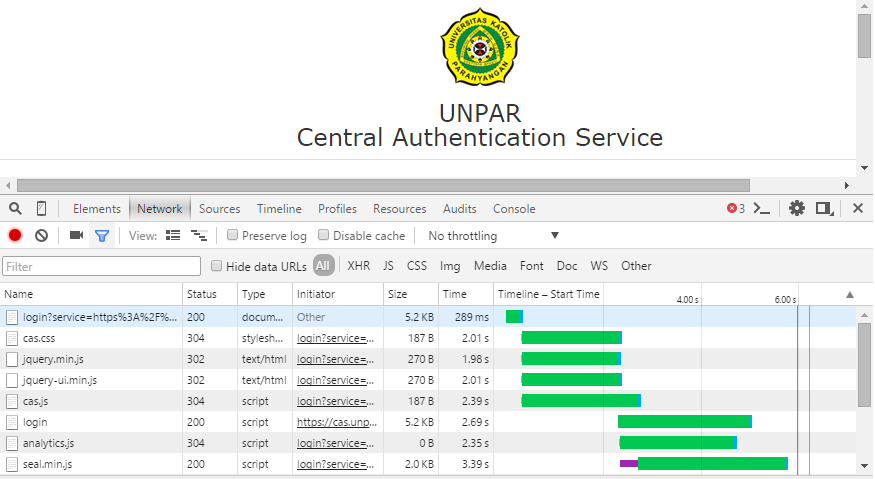
\includegraphics[scale=0.5]{Gambar/chrome-devtools}
	\caption{Chrome DevTools} 
	\label{fig:chrome_devtools}
\end{figure}

\section{Play Framework}
\label{sec:play}

Play Framework \cite{Leroux:2014} merupakan sebuah web framework berbasis Java dan Scala. Play juga menggunakan \textit{design pattern} Model-View-Controller (MVC) di mana \textit{model} dan \textit{controller} menggunakan Java sedangkan \textit{view} menggunakan Scala dan HTML. 
}{}
\ifdefstring{\vbabc}{1}{\chapter{Analisis}
\label{chap:analisis}

\section{Analisis Portal Akademik Mahasiswa}
Portal Akademik Mahasiswa merupakan sebuah situs jaringan yang diperuntukan bagi mahasiswa dalam rangka mendapatkan informasi kegiatan akademik\cite{BTI:2012}. Mahasiswa dapat mengakses Portal Akademik Mahasiswa melalui URL \url{https://studentportal.unpar.ac.id/}. Untuk mengakses Portal Akademik Mahasiswa, mahasiswa harus \textit{login} menggunakan akun email \textit{student}. Halaman \textit{login} Student Portal UNPAR terintegrasi dengan CAS (\textit{Central Authentication Service}) UNPAR\footnote{\url{https://cas.unpar.ac.id}}.

\begin{figure}[H]
	\centering
	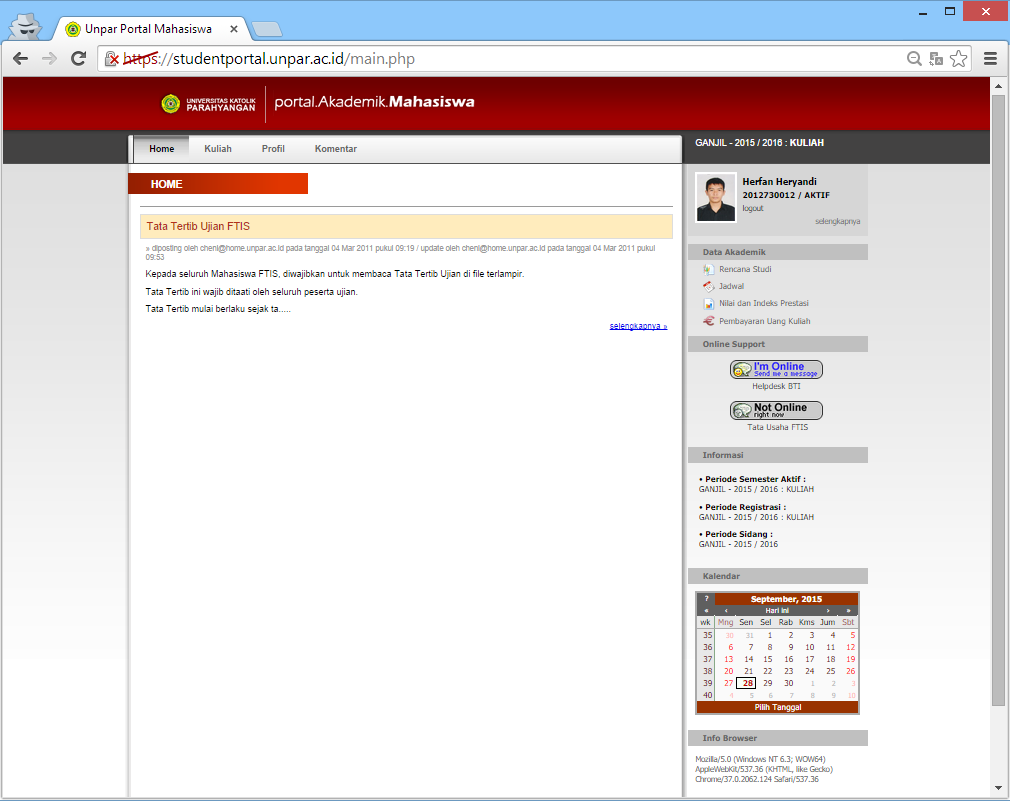
\includegraphics[scale=0.5]{Gambar/pam-home}
	\caption{Halaman Utama Portal Akademik Mahasiswa} 
	\label{fig:3_pam_home}
\end{figure}

Pada halaman utama Portal Akademik Mahasiswa (gambar \ref{fig:3_pam_home}), terdapat beberapa bagian yaitu:
\begin{enumerate}
	\item Menu Atas\\
	Menu ini berfungsi sebagai menu pendukung yang terdiri dari : 
	\begin{itemize}
		\item \textbf{Home}, menampilkan informasi atau pengumuman yang dikeluarkan oleh fakultas masing-masing (Gambar \ref{fig:3_pam_atas_home}). 
		
		\begin{figure}[H]
			\centering
			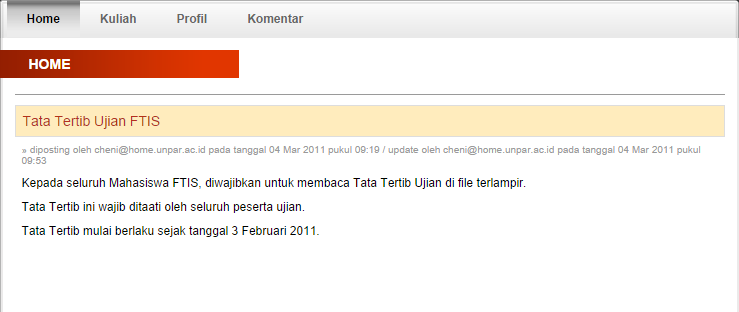
\includegraphics[scale=0.5]{Gambar/pam-atas-home}
			\caption{Menu Atas Home} 
			\label{fig:3_pam_atas_home}
		\end{figure}
		
		\item \textbf{Kuliah}, menampilkan pengumuman per mata kuliah sesuai dengan mata kuliah dan kelas yang diambil oleh masing-masing mahasiswa (Gambar \ref{fig:3_pam_atas_kuliah}).  
		
		\begin{figure}[H]
			\centering
			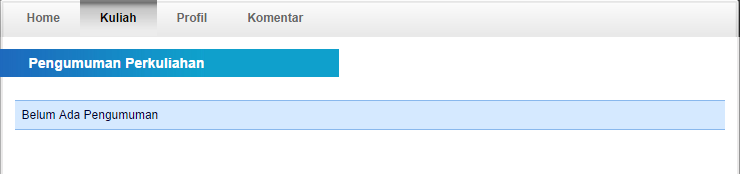
\includegraphics[scale=0.5]{Gambar/pam-atas-kuliah}
			\caption{Menu Atas Kuliah} 
			\label{fig:3_pam_atas_kuliah}
		\end{figure}
		
		\item \textbf{Profil}, berisi tentang data diri masing-masing mahasiswa (Gambar \ref{fig:3_pam_atas_profil}). 
		
		\begin{figure}[H]
			\centering
			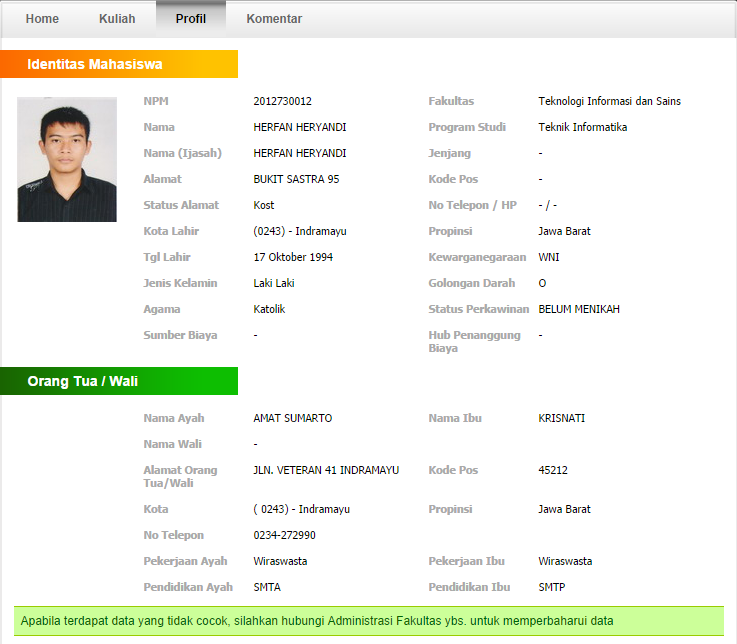
\includegraphics[scale=0.5]{Gambar/pam-atas-profil}
			\caption{Menu Atas Profil} 
			\label{fig:3_pam_atas_profil}
		\end{figure}
		
		\item \textbf{Komentar}, berisi komentar, saran, dan kritik dari mahasiswa (Gambar \ref{fig:3_pam_atas_komentar}).
		
		\begin{figure}[H]
			\centering
			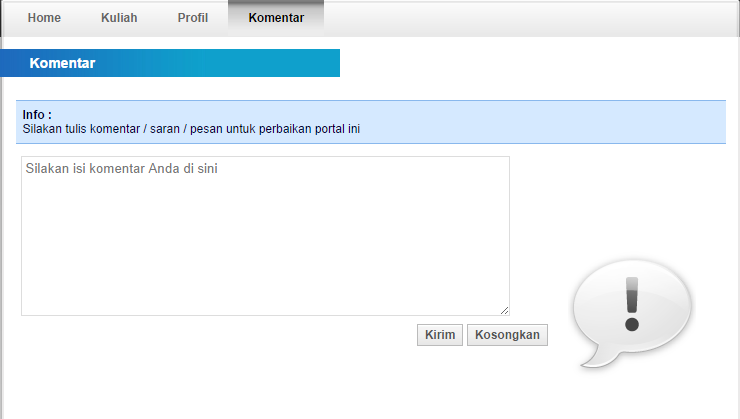
\includegraphics[scale=0.5]{Gambar/pam-atas-komentar}
			\caption{Menu Atas Komentar} 
			\label{fig:3_pam_atas_komentar}
		\end{figure}

	\end{itemize}
	
	\item Identitas Portal \\
	Bagian ini menampilkan identitas pengguna portal. Tampilan identitas ini dapat ditampilkan lengkap dengan melakukan klik pada \textit{link} ``selengkapnya'' atau ditampilkan minimal dengan klik \textit{link} ``tutup''. Identitas yang ditampilkan adalah nama, Nomor Pokok Mahasiswa (NPM), status keaktifan, pas foto, email, dosen wali, program studi, dan fakultas seperti yang terlihat pada gambar \ref{fig:3_pam_identitas}.   
	\begin{figure}[H]
			\centering
			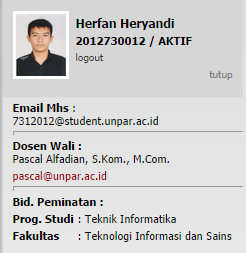
\includegraphics[scale=0.75]{Gambar/pam-identitas}
			\caption{Identitas Portal} 
			\label{fig:3_pam_identitas}
		\end{figure}
		
	\item Menu Utama\\
	Bagian ini memuat fitur utama Portal Akademik Mahasiswa mengenai data akademik (gambar \ref{fig:3_pam_utama}) yang terdiri dari:
		\begin{figure}[H]
			\centering
			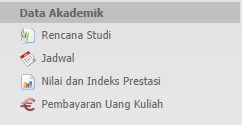
\includegraphics[scale=0.75]{Gambar/pam-utama}
			\caption{Menu Utama} 
			\label{fig:3_pam_utama}
		\end{figure}
	\begin{itemize}
	
		\item \textbf{Rencana Studi}\\
		Menu Rencana Studi terdiri dari submenu: 
		\begin{itemize}
			\item Registrasi (FRS/PRS)\\
			Digunakan sebagai formulir pengisian rencana studi awal (FRS) dan perubahan rencana studi (PRS) (Gambar \ref{fig:3_pam_utama_registrasi}). 			
			\begin{figure}[H]
				\centering
				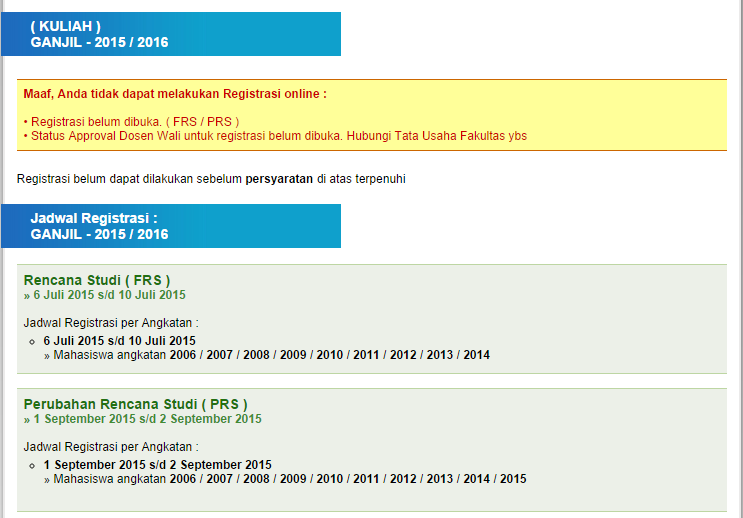
\includegraphics[scale=0.5]{Gambar/pam-utama-rencanastudi}
				\caption{Tampilan Registrasi FRS/PRS} 
				\label{fig:3_pam_utama_registrasi}
			\end{figure}
			
			\item Kartu Rencana Studi \\
			Menampilkan informasi mata kuliah yang telah diambil melalui submenu Registrasi (Gambar \ref{fig:3_pam_utama_krs}). Kartu Rencana Studi juga dapat dicetak melalui submenu ini. 
			\begin{figure}[H]
				\centering
				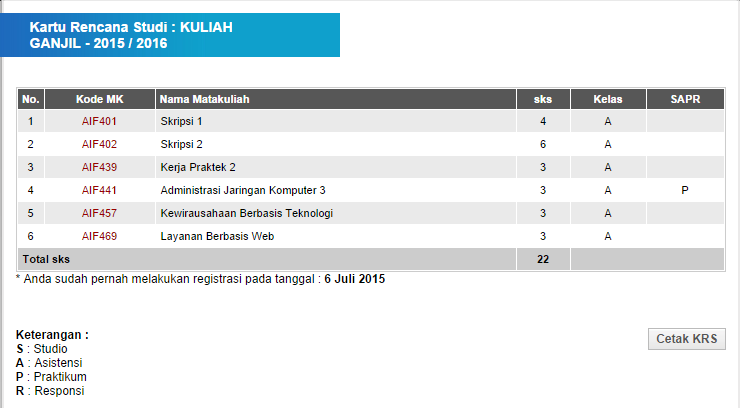
\includegraphics[scale=0.5]{Gambar/pam-utama-krs}
				\caption{Tampilan Kartu Rencana Studi\cite{BTI:2012}} 
				\label{fig:3_pam_utama_krs}
			\end{figure}
			
			\item Pindah Kelas MKU \\
			Mahasiswa dapat memilih kelas yang masih tersedia di kolom Jadwal Baru dan menekan tombol ``Simpan'' untuk setiap kelas yang diubah (Gambar \ref{fig:3_pam_utama_pindahmku}). 
			\begin{figure}[H]
				\centering
				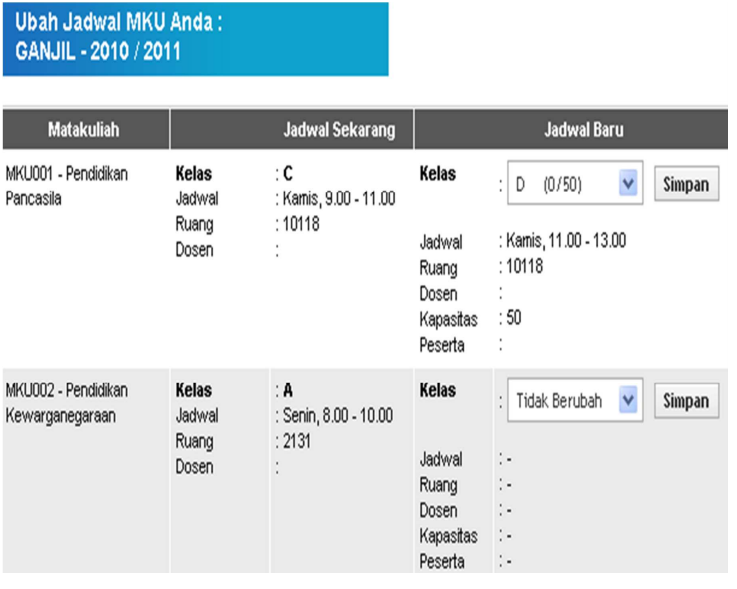
\includegraphics[scale=0.5]{Gambar/pam-utama-pindahmku}
				\caption{Tampilan Pindah Kelas MKU\cite{BTI:2012}} 
				\label{fig:3_pam_utama_pindahmku}
			\end{figure}

		\end{itemize}
		
		\item \textbf{ Jadwal}\\
		Menu Jadwal terdiri dari submenu: 
		\begin{itemize}
			\item Kuliah, UTS, dan UAS \\
			Submenu ini berisi tentang jadwal kuliah, UTS dan UAS yang dapat disusun per semester (Gambar \ref{fig:3_pam_utama_jadwal}). 
			\begin{figure}[H]
				\centering
				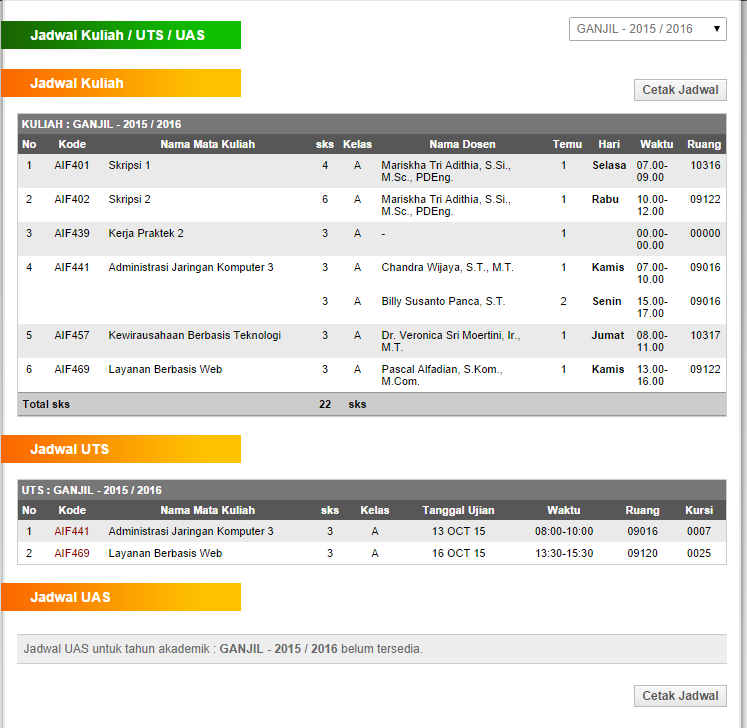
\includegraphics[scale=0.5]{Gambar/pam-utama-jadwal}
				\caption{Tampilan Jadwal Kuliah, UTS, dan UAS} 
				\label{fig:3_pam_utama_jadwal}
			\end{figure}
			
			\item MKU \\
			Submenu ini menampilkan seluruh jadwal Mata Kuliah Umum (MKU) yang memberikan informasi tentang kelas-kelas yang dibuka oleh Pusat Kajian Humaniora (PKH) (Gambar \ref{fig:3_pam_utama_jadwalmku}). 
			\begin{figure}[H]
				\centering
				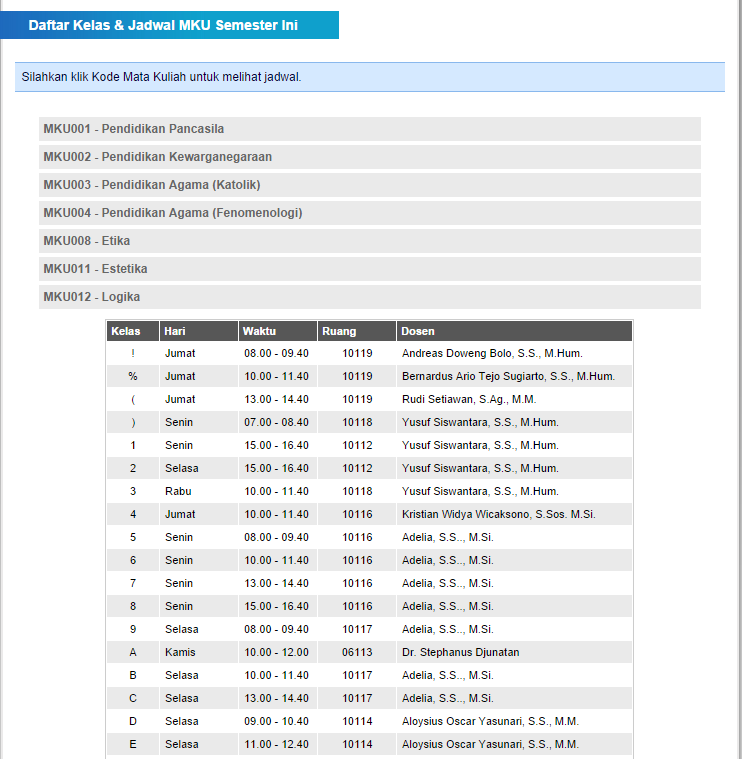
\includegraphics[scale=0.5]{Gambar/pam-utama-jadwalmku}
				\caption{Tampilan Jadwal MKU} 
				\label{fig:3_pam_utama_jadwalmku}
			\end{figure}
			
			\item Seluruh Fakultas \\
			Fitur ini memberikan informasi mengenai jadwal-jadwal yang ada di seluruh fakultas (Gambar \ref{fig:3_pam_utama_jadwalall}).
			\begin{figure}[H]
				\centering
				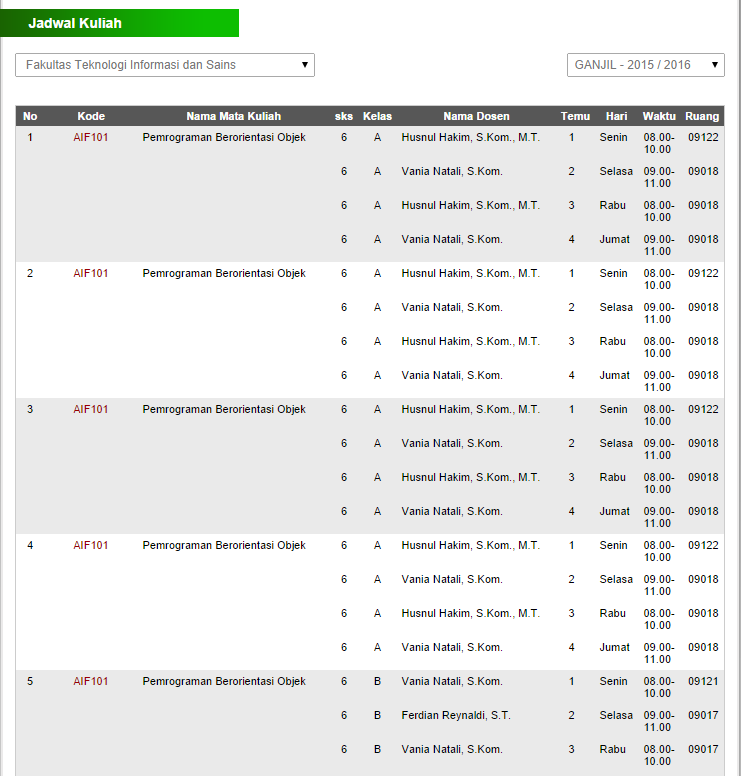
\includegraphics[scale=0.5]{Gambar/pam-utama-jadwalall}
				\caption{Tampilan Jadwal Seluruh Fakultas} 
				\label{fig:3_pam_utama_jadwalall}
			\end{figure}
		\end{itemize}
		
		\item \textbf{Nilai dan Indeks Prestasi}\\
		Menu Nilai dan Indeks Prestasi terdiri dari submenu: 
		\begin{itemize}
			\item Riwayat per Semester \\
			Submenu ini menampilkan informasi nilai per semester. Mahasiswa dapat melihat nilai sesuai dengan semester yang dipilih atau bisa memilih
pilihan ``Seluruh Tahun Akademik'' untuk melihat seluruh nilai berdasarkan semester (Gambar \ref{fig:3_pam_utama_nilai}).
			\begin{figure}[H]
				\centering
				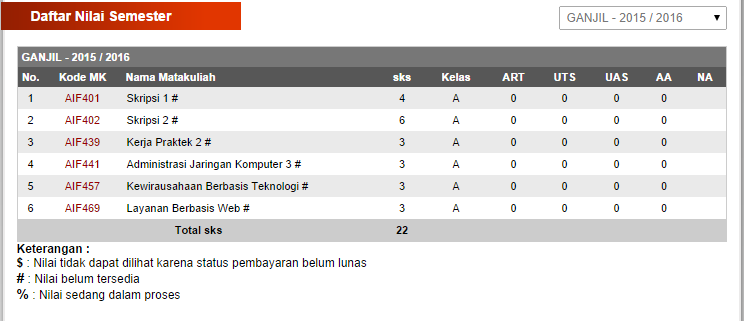
\includegraphics[scale=0.5]{Gambar/pam-utama-nilai}
				\caption{Tampilan Riwayat Per Semester} 
				\label{fig:3_pam_utama_nilai}
			\end{figure}
			
			\item Daftar Perkembangan Studi \\
			Seluruh riwayat mata kuliah dan nilai yang pernah ditempuh ditampilkan di submenu ini (Gambar \ref{fig:3_pam_utama_dps}). Pada bagian bawah halaman, terdapat statistik nilai dan indeks prestasi (Gambar \ref{fig:3_pam_utama_dpsstat}). 
			\begin{figure}[H]
				\centering
				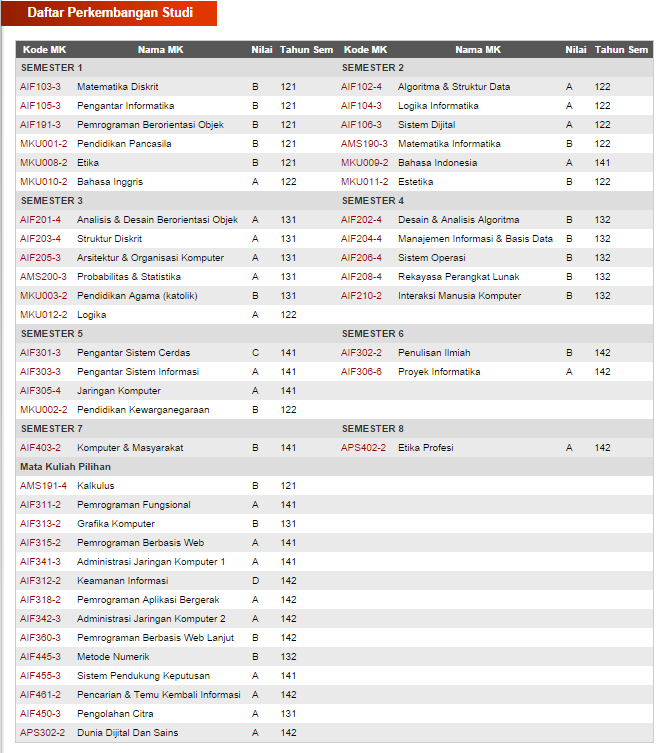
\includegraphics[scale=0.5]{Gambar/pam-utama-dps}
				\caption{Tampilan Daftar Perkembangan Studi} 
				\label{fig:3_pam_utama_dps}
			\end{figure}
			
			\begin{figure}[H]
				\centering
				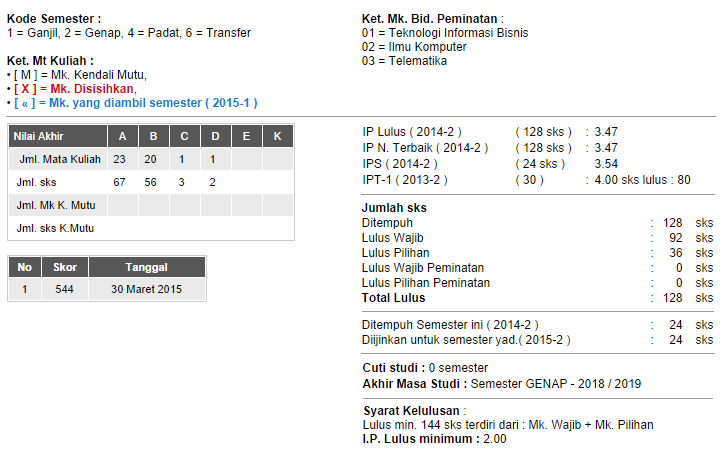
\includegraphics[scale=0.5]{Gambar/pam-utama-dpsstat}
				\caption{Tampilan Statistik Nilai dan IP} 
				\label{fig:3_pam_utama_dpsstat}
			\end{figure}
			
			\item Riwayat Indeks Prestasi \\
			Menampilkan daftar riwayat indeks prestasi semester dan kumulatif setiap semester. Tampilan ini juga dilengkapi dengan grafik perkembangan (Gambar \ref{fig:3_pam_utama_ip}). 
			\begin{figure}[H]
				\centering
				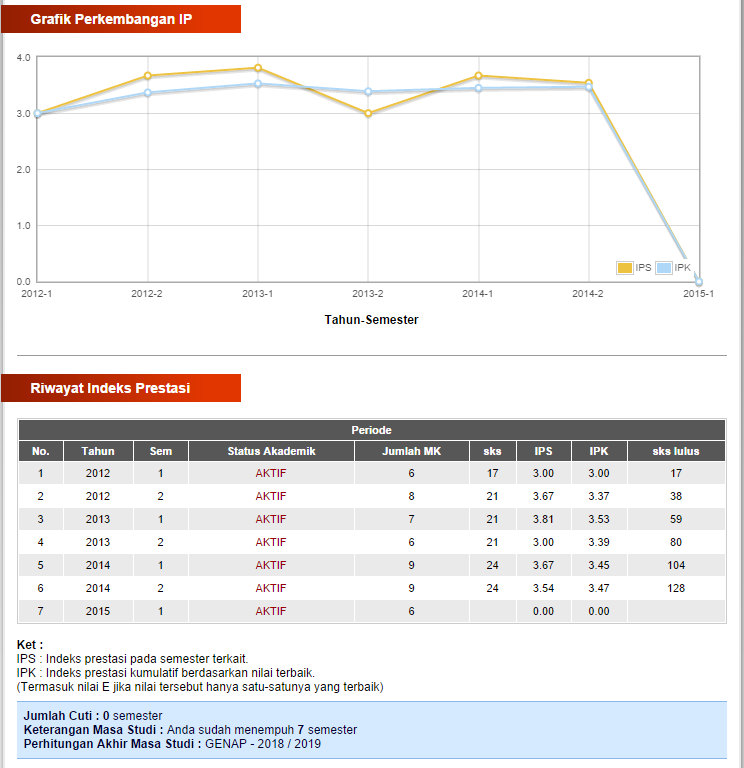
\includegraphics[scale=0.5]{Gambar/pam-utama-ip}
				\caption{Tampilan Riwayat Indeks Prestasi} 
				\label{fig:3_pam_utama_ip}
			\end{figure}
			
			\item TOEFL \\
			Menampilkan daftar riwayat skor \textit{Test of English as Foreign Language} (TOEFL) yang pernah ditempuh (Gambar \ref{fig:3_pam_utama_toefl}). Mahasiswa diwajibkan untuk menempuh TOEFL dengan skor minimal 500.
			
			\begin{figure}[H]
				\centering
				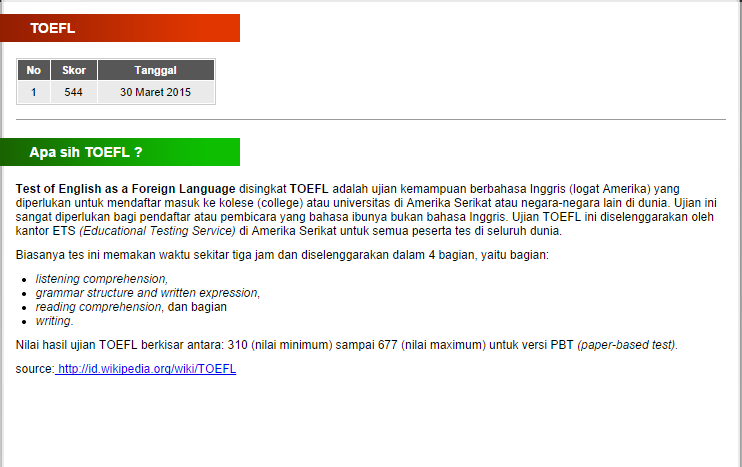
\includegraphics[scale=0.5]{Gambar/pam-utama-toefl}
				\caption{Tampilan TOEFL} 
				\label{fig:3_pam_utama_toefl}
			\end{figure}
		\end{itemize}
		
		\item \textbf{Pembayaran Uang Kuliah}\\
		Menu ini berfungsi untuk melihat data tagihan pembayaran uang kuliah serta cara-cara pembayarannya (Gambar \ref{fig:3_pam_utama_pembayaran}).
		\begin{figure}[H]
				\centering
				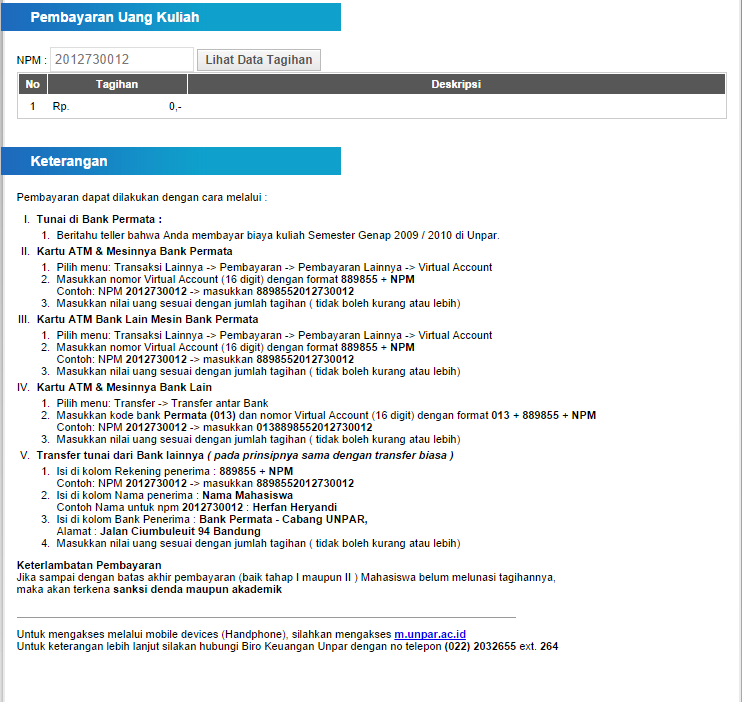
\includegraphics[scale=0.5]{Gambar/pam-utama-pembayaran}
				\caption{Tampilan Pembayaran Uang Kuliah} 
				\label{fig:3_pam_utama_pembayaran}
			\end{figure}
		\end{itemize}
		
	\item \textbf{Informasi}\\
		Bagian ini menampilkan informasi tentang periode-periode yang sedang aktif (Gambar \ref{fig:3_pam_utama_informasi}). Sebagai contoh jika ``Periode Registrasi'' diklik maka akan muncul \textit{pop up} seperti pada gambar \ref{fig:3_pam_utama_informasipop}.
			\begin{figure}[H]
				\centering
				
\includegraphics[scale=0.75]{Gambar/pam-utama-informasi}
				\caption{Tampilan Informasi} 
				\label{fig:3_pam_utama_informasi}
			\end{figure}
			
			\begin{figure}[H]
				\centering
				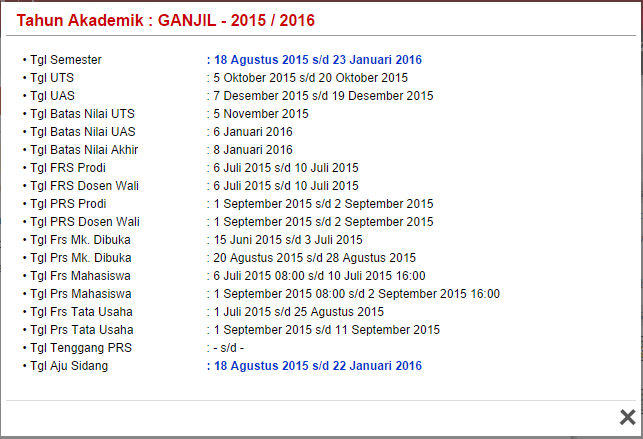
\includegraphics[scale=0.5]{Gambar/pam-utama-infopop}
				\caption{Tampilan \textit{Pop Up} Informasi} 
				\label{fig:3_pam_utama_informasipop}
			\end{figure}
		
	\item \textbf{Kalender}\\
		Bagian ini menampilkan kalender masehi (Gambar \ref{fig:3_pam_utama_kalender}).
		\begin{figure}[H]
				\centering
				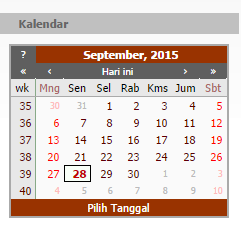
\includegraphics[scale=0.75]{Gambar/pam-utama-kalender}
				\caption{Tampilan Kalender} 
				\label{fig:3_pam_utama_kalender}
			\end{figure}
		
	\item \textbf{Info Browser}\\
		Bagian ini menampilkan informasi tentang internet \textit{browser} yang digunakan pada saat membuka Portal Akademik Mahasiswa (Gambar \ref{fig:3_pam_utama_infobrowser}). 
		\begin{figure}[H]
				\centering
				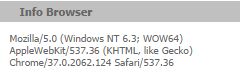
\includegraphics[scale=0.75]{Gambar/pam-utama-infobrowser}
				\caption{Tampilan Info Browser} 
				\label{fig:3_pam_utama_infobrowser}
			\end{figure}
\end{enumerate}

\section{Analisis Kebutuhan Informatika Student Portal}
\label{sec:kebutuhan}
Dalam menganalisis kebutuhan Informatika Student Portal, penulis melakukan wawancara dengan mahasiswa Program Studi Teknik Informatika UNPAR. Sampel yang diambil adalah lima orang mahasiswa dari setiap angkatan dalam empat tahun terakhir yaitu angkatan 2012 sampai 2015. Setelah melakukan wawancara, penulis memperoleh fitur-fitur yang diinginkan mahasiswa antara lain:
\begin{enumerate}
	\item Prasyarat mata kuliah\\
	Mahasiswa bisa memeriksa prasyarat mata kuliah saat FRS sehingga tidak terjadi kesalahan pengambilan mata kuliah. Prasyarat mata kuliah yang ditampilkan di Portal Akademik Mahasiswa kurang akurat. Selain itu, dari 20 mahasiswa yang diwawancara, hanya ada satu mahasiswa yang mengetahui bahwa Portal Akademik Mahasiswa memiliki fitur prasyarat. Prasyarat mata kuliah untuk Program Studi Teknik Informatika juga tersedia di \url{http://tinyurl.com/lionov}\footnote{\url{http://tinyurl.com/lionov}, diakses 5 September 2015}, namun mahasiswa merasa kurang praktis karena harus memeriksa secara manual. Mahasiswa menginginkan agar fitur ini bisa dibuat untuk mempermudah FRS. Fitur ini akan menampilkan seluruh mata kuliah yang dibuka pada semester terkini beserta status pengambilannya.
	\item Ringkasan data akademik\\
	Ringkasan data akademik menampilkan data mengenai mata kuliah pilihan wajib dan sisa SKS untuk mencapai kelulusan. Mahasiswa menginginkan fitur ini dibuat untuk membantu mereka dalam mengatur perkuliahannya.
	\item Perubahan IPS dan IPK berdasarkan riwayat nilai\\
	Dalam Portal Akademik Mahasiswa, nilai pertama kali muncul dalam riwayat nilai. Riwayat IP tidak berubah secara otomatis saat seluruh nilai di riwayat nilai sudah muncul. Mahasiswa menginginkan agar IPS dan IPK dapat berubah secara otomatis saat nilai muncul.
	\item Jadwal kuliah yang tersusun\\
	Tampilan jadwal kuliah dalam Portal Akademik Mahasiswa tidak terurut berdasarkan hari seperti pada gambar \ref{fig:3_jadwal_portal} sehingga perlu direkapitulasi lagi. Mahasiswa menginginkan agar tampilan jadwal tersusun dan dalam bentuk seperti gambar \ref{fig:3_jadwal_rekap}.
		\begin{figure}[H]
			\centering
			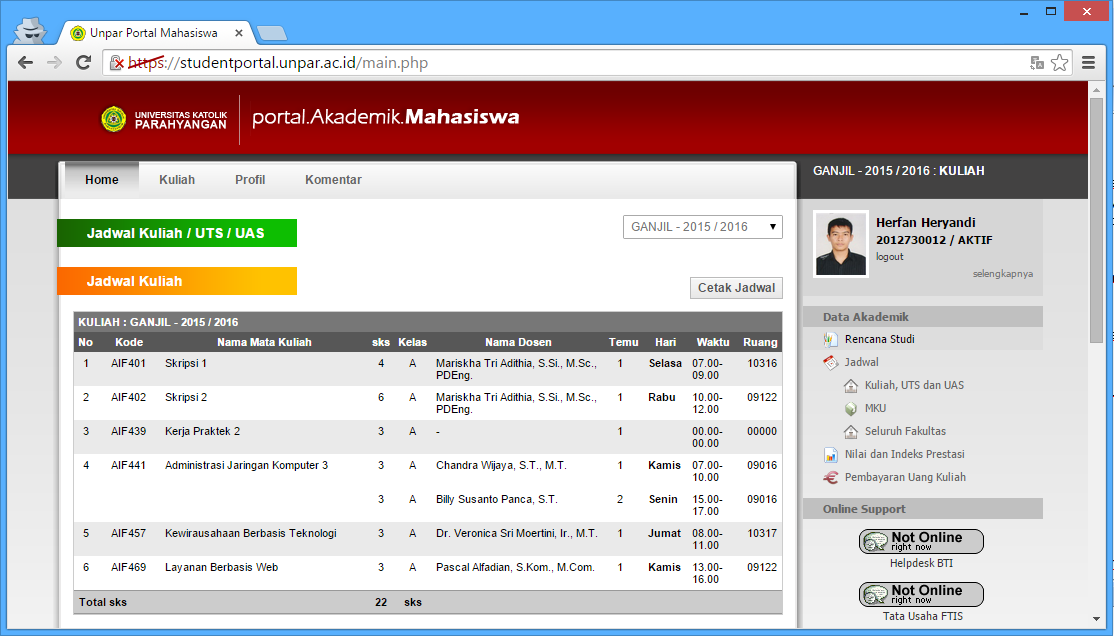
\includegraphics[scale=0.5]{Gambar/jadwal-portal}
			\caption{Tampilan Jadwal pada Portal Akademik Mahasiswa} 
			\label{fig:3_jadwal_portal}
		\end{figure}
		
		\begin{figure}[H]
			\centering
			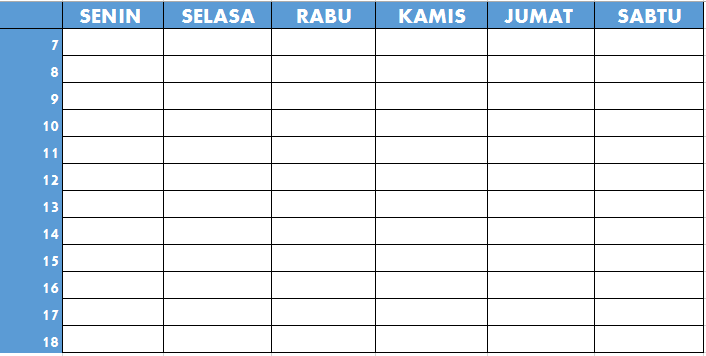
\includegraphics[scale=0.5]{Gambar/jadwal-rekap}
			\caption{Tampilan Jadwal yang Diinginkan Mahasiswa} 
			\label{fig:3_jadwal_rekap}
		\end{figure}
		
	\item Kalender akademik\\
	Kalender akademik merupakan salah satu fitur pada Portal Akademik Mahasiswa namun sekarang fitur tersebut sudah tidak ada lagi. Mahasiswa menginginkan fitur kalender akademik kembali untuk mengetahui tanggal-tanggal penting pada perkuliahan. 
	\item Rincian pembayaran\\
	Tagihan pada Portal Akademik Mahasiswa tidak mencantumkan batas akhir pembayaran dan rincian nominal tagihan. Mahasiswa menginginkan rincian pembayaran agar tidak terlambat membayar uang kuliah dan dapat mengetahui rincian nominal tagihan.
	\item Rincian mata kuliah\\
	Setiap mata kuliah yang dibuka memiliki rincian seperti deskripsi mata kuliah dan jenis mata kuliah yaitu apakah mata kuliah tersebut wajib, pilihan, atau pilihan wajib. Mahasiswa menginginkan fitur ini agar dapat mengetahui mata kuliah apa yang akan dipelajari.
	\item Tampilan situs web sama di sistem operasi manapun\\
	Jika tidak menggunakan sistem operasi Windows seperti Linux dan Mac, saat mengakses Portal Akademik Mahasiswa melalui \url{https://studentportal.unpar.ac.id/}, maka mahasiswa akan diarahkan ke \url{https://m.studentportal.unpar.ac.id/} yaitu Portal Akademik Mahasiswa dengan tampilan \textit{mobile} (Gambar \ref{fig:3_pam_mobile}). Tampilan ini tidak memiliki fitur selengkap Portal Akademik Mahasiswa, hanya memiliki fitur pengumunan kuliah, jadwal kuliah, UTS, dan UAS, nilai, IP, dan tagihan. Selain itu, tampilan \textit{mobile} pada telepon seluler akan terlihat sangat kecil sehingga tidak sulit untuk memilih menu. Mahasiswa menginginkan fitur ini agar Informatika Student Portal dapat diakses di sistem operasi manapun tanpa perubahan tampilan.
	\begin{figure}[H]
			\centering
			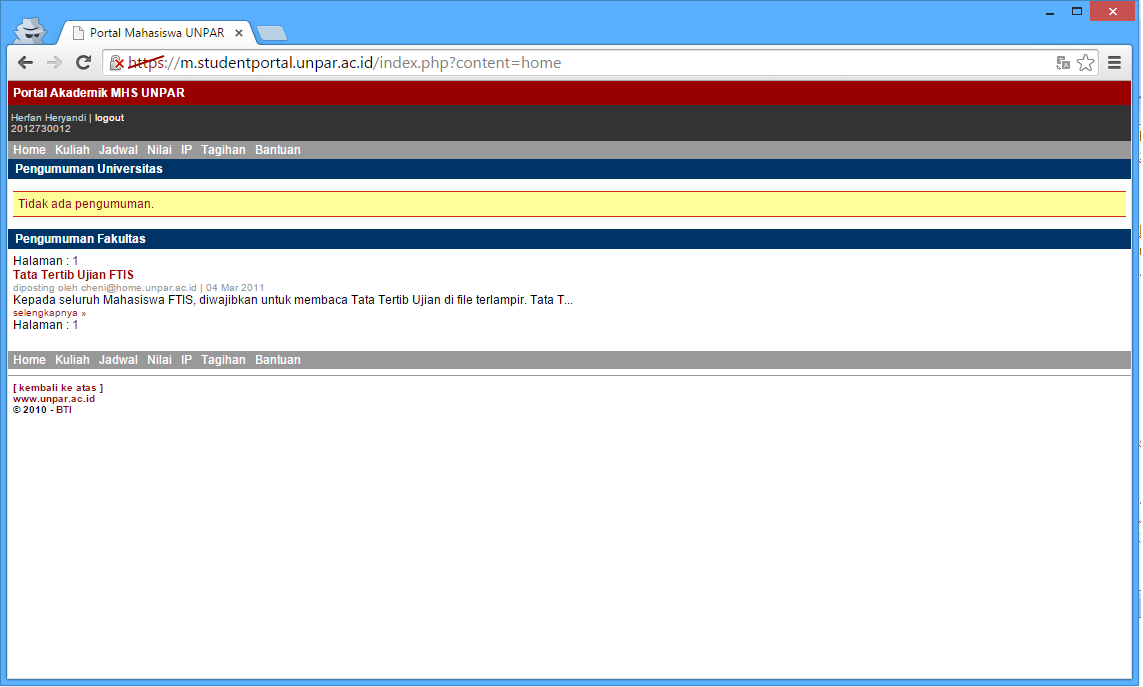
\includegraphics[scale=0.5]{Gambar/pam-mobile}
			\caption{Tampilan \textit{Mobile} Portal Akademik Mahasiswa} 
			\label{fig:3_pam_mobile}
		\end{figure}
	\item Kontak dosen\\
	Kontak dosen berisi informasi email setiap dosen sehingga dapat mempermudah mahasiswa untuk menghubungi dosen. Mahasiswa juga dapat mengirim email secara langsung melalui Portal Akademik Mahasiswa.
	\item Pohon kurikulum\\
	Mahasiswa munginnginkan agar dapat melihat pohon kurikulum Program Studi Teknik Informatika dalam Portal Akademik Mahasiswa.
	\item Pemberitahuan\\
	Mahasiswa menginginkan Portal Akademik Mahasiswa menampilkan pemberitahuan berupa \textit{pop up} mengenai pengumuman terkini.
	\item Unggah \textit{Curriculum Vitae}
	Mahasiswa menginginkan agar dapat mengunggah data mengenai kegiatan dan keaktifan di universitas agar dapat digunakan oleh perusahaan untuk mencari mahasiswa dengan kriteria tertentu misalnya untuk kepentingan magang dan beasiswa.
\end{enumerate}

Penulis menetapkan fitur-fitur yang akan dipilih untuk diimplementasikan harus memenuhi kriteria:
\begin{itemize}
	\item Data yang dibutuhkan dapat diambil dari Portal Akademik Mahasiwa \\
	Aplikasi Informatika Student Portal merupakan aplikasi hasil kustomisasi Portal Akademik Mahasiswa. Informasi yang ditampilkan Informatika Student Portal diperoleh dengan cara mengolah data dari Portal Akademik Mahasiswa. Jadi data yang dibutuhkan Informatika Student Portal harus dapat diambil dari Portal Akademik Mahasiswa. 
	\item Data hasil olahan tidak tersedia di Portal Akademik Mahasiswa\\
	Jika data hasil olahan yang sudah tersedia di Portal Akademik Mahasiswa, maka fitur tidak perlu dibuat lagi di Informatika Student Portal karena mahasiswa dapat mengakses langsung Portal Akademik Mahasiswa.
	\item Fitur mendukung fungsi Portal Akademik Mahasiswa sebagai sumber informasi akademik \\
	Portal Akademik Mahasiswa berfungsi sebagai sumber informasi akademik karena itu Informatika Student Portal juga harus mememiliki fitur yang dapat mendukung fungsi tersebut.
\end{itemize}

Hasil analisis fitur-fitur yang diinginkan berdasarkan kriteria di atas dan batas waktu pembangunan aplikasi dapat dilihat pada tabel \ref{tab:3_hasil_fitur}.
\begin{table}[H]
	\centering
		\caption{Tabel Hasil Analisis Kebutuhan Informatika Student Portal}
    \begin{tabular}{|p{4.5cm}|p{2.5cm}|p{8cm}|}
		\hline
		Fitur & Dibuat/Tidak dibuat & Alasan\\
		\hline
		Prasyarat mata kuliah                             & Dibuat       & Data dapat diambil dari Portal Akademik Mahasiswa dan aturan prasyarat mata kuliah Program Studi Teknik Informatika sudah tersedia di SIA Models                   \\
		\hline
    Ringkasan data akademik                               & Dibuat       & Data dapat diambil dari Portal Akademik Mahasiswa dan didukung oleh SIA Models                        \\
		\hline
    Perubahan IPS dan IPK berdasarkan riwayat nilai   & Dibuat       &  IPS dan IPK dapat dihitung melalui riwayat nilai yang dapat diperoleh dari Portal Akademik Mahasiswa \\
		\hline
    Jadwal kuliah yang tersusun                       & Dibuat       & Jadwal yang tersusun mempermudah mahasiswa untuk                                                      \\
		\hline
    Kalender akademik                                 & Tidak dibuat & Data tidak bisa diperoleh dari Portal Akademik Mahasiwa                                               \\
		\hline
    Rincian pembayaran                                & Tidak dibuat & Data tidak bisa diperoleh dari Portal Akademik Mahasiwa                                               \\
		\hline
    Rincian mata kuliah                               & Tidak dibuat & Data tidak bisa diperoleh dari Portal Akademik Mahasiwa                                               \\
		\hline
    Tampilan situs web sama di sistem operasi manapun & Dibuat       & Aplikasi yang akan dibuat merupakan situs web yang responsif                                          \\
		\hline
    Kontak dosen                                      & Tidak dibuat & Data tidak bisa diperoleh dari Portal Akademik Mahasiwa                                               \\
		\hline
    Pemberitahuan                                     & Tidak dibuat & Waktu pengerjaan yang terbatas                                                                        \\
		\hline
    Unggah \textit{Curriculum Vitae}                           & Tidak dibuat & Tidak mendukung Portal Akademik Mahasiswa sebagai sumber informasi akademik                           \\
		\hline
		\end{tabular}
	\label{tab:3_hasil_fitur}
\end{table}


\section{Analisis Komunikasi Portal Akademik Mahasiswa untuk Fitur Informatika Student Portal}
Untuk memenuhi fitur Informatika Student Portal, peneliti menganalisis komunikasi Portal Akademik Mahasiswa ke dalam beberapa kasus yang akan dijelaskan pada subbab-subbab berikut.

\subsection{Kasus \textit{Login}}
Di Portal Akademik Mahasiswa, mahasiswa dapat \textit{login} dengan cara:
\begin{enumerate}
	\item Mengakses \url{https://studentportal.unpar.ac.id/} dan mengklik tombol ``input\#submit.login-button'' (Gambar \ref{fig:3_case_login}).
	\begin{figure}[H]
			\centering
			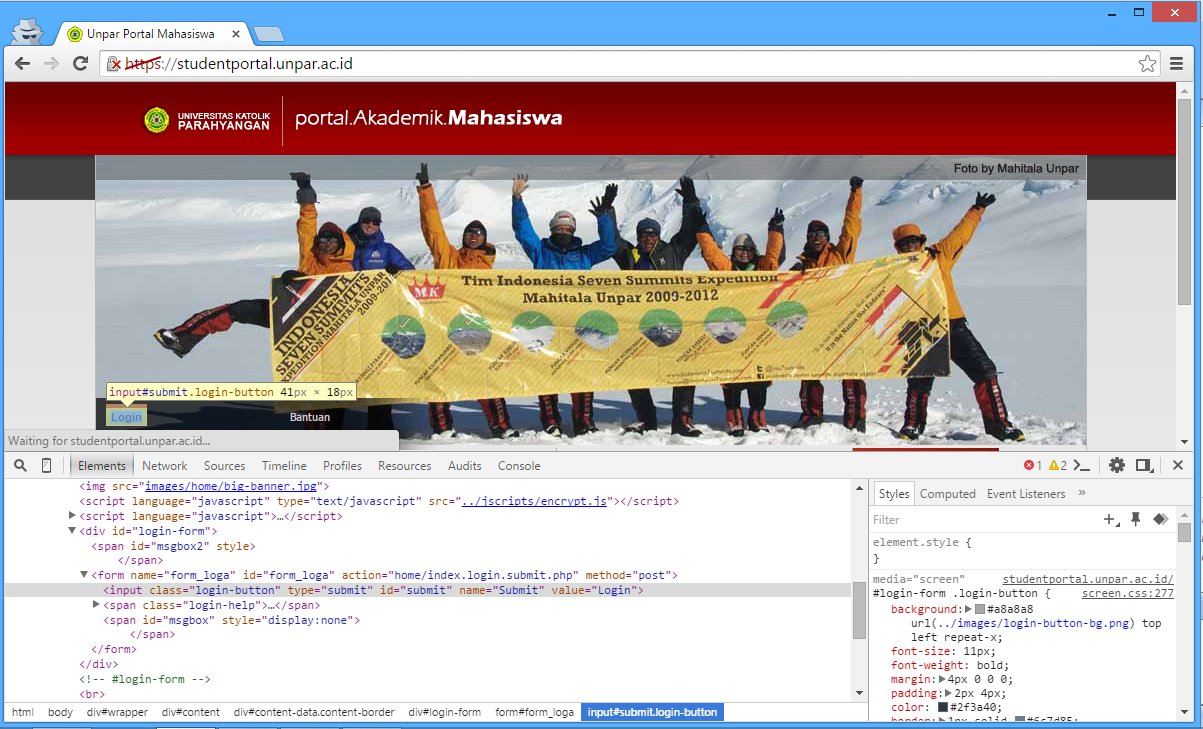
\includegraphics[scale=0.5]{Gambar/case-login}
			\caption{Tombol ``input\#submit.login-button'' pada Halaman Depan Portal Akademik Mahasiswa} 
			\label{fig:3_case_login}
		\end{figure}
		
	\item Saat tombol tersebut ditekan, mahasiswa akan dibawa ke halaman \url{index.login.submit.php} dengan \textit{form data} berisi:
			\begin{itemize}
				\item Submit: selalu berisi ``Login''
			\end{itemize}
		
	\item Secara otomatis halaman akan berpindah lagi ke \url{https://cas.unpar.ac.id/login? service=https\%3A\%2F\%2Fstudentportal.unpar.ac.id\%2Fhome\%2Findex.login.submit.php}.
		
	\item Di sana, akan ditampilkan halaman \textit{login} CAS UNPAR di mana mahasiswa diminta mengisi \textit{``Username''} pada kolom ``input\#username.required'' dan \textit{``Password''} pada kolom ``input\#password.required'' (Gambar \ref{fig:3_case_login_cas}).
	\begin{figure}[H]
			\centering
			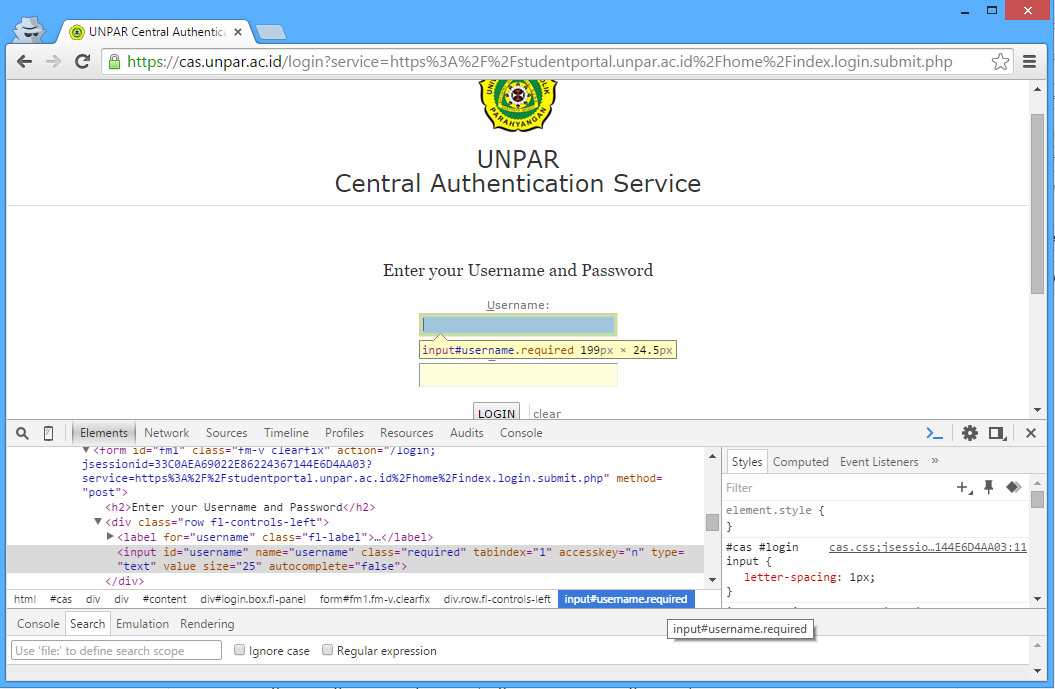
\includegraphics[scale=0.5]{Gambar/case-login-cas}
			\caption{Kolom \textit{``Username''} ``input\#username.required'' pada Halaman CAS UNPAR} 
			\label{fig:3_case_login_cas}
		\end{figure}
	\item Setelah itu mahasiswa harus menekan tombol ``input.btn-submit''. Data tersebut akan dikirimkan ke \url{/login;jsessionid=...?service=https://studentportal.unpar.ac.id/home/index.login.submit.php} dengan \textit{cookie}:
	\begin{itemize}
		\item JSESSIONID: diambil dari \textit{cookie} yang di-\textit{set} pada halaman \url{https://cas.unpar.ac.id/login? service=https\%3A\%2F\%2Fstudentportal.unpar.ac.id\%2Fhome\%2Findex.login.submit.php}
	\end{itemize}
	 Data yang dikirim juga mengandung \textit{form data} sebagai berikut (Gambar \ref{fig:3_case_form}):
	\begin{itemize}
		\item username: diambil dari nilai elemen ``input\#username.required''
		\item password: diambil dari nilai elemen ``input\#password.required''
		\item lt: diambil dari nilai elemen ``input'' dengan nama ``lt''
		\item execution: diambil dari nilai elemen ``input'' dengan nama ``execution''
		\item \_eventId: selalu berisi ``submit''
		\item submit: selalu berisi ``LOGIN''
		\begin{figure}[H]
			\centering
			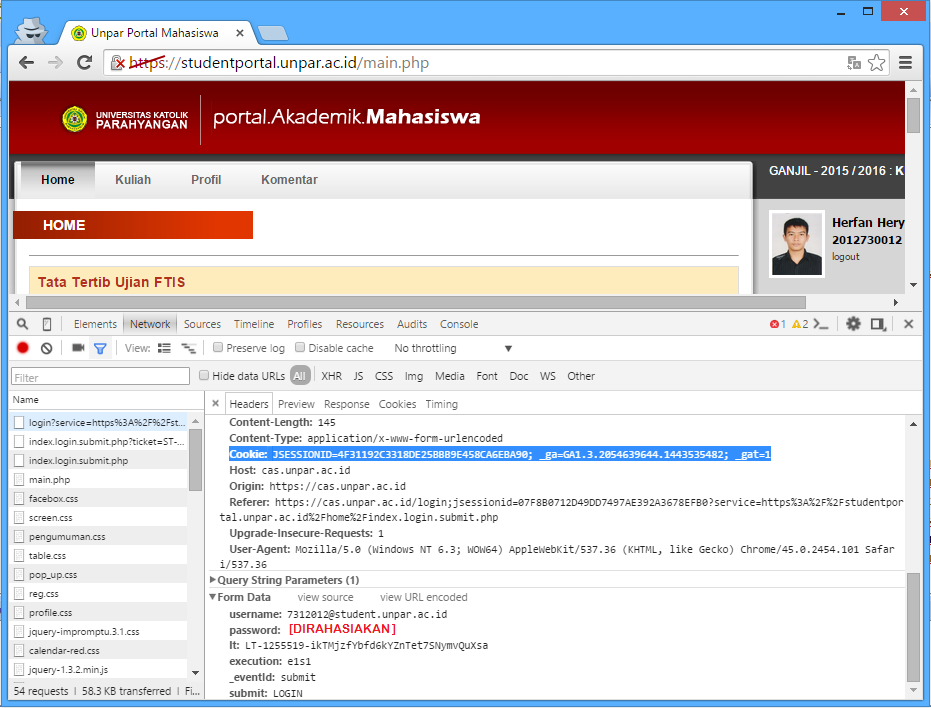
\includegraphics[scale=0.5]{Gambar/case-form}
			\caption{\textit{Form Data} yang dikirim CAS UNPAR} 
			\label{fig:3_case_form}
		\end{figure}
	\end{itemize}
\item Jika berhasil, akan dilakukan pengalihan beberapa kali dan diakhiri di \url{https://studentportal.unpar.ac.id/main.php} dengan \textit{cookie} sebagai berikut:
\begin{itemize}
	\item PHPSESSID: diambil dari \textit{cookie} yang di-\textit{set} pada beberapa pengalihan sebelumnya
	\item \_ga dan \_gat: tidak diperlukan, digunakan oleh Google Analytics\footnote{\url{https://developers.google.com/analytics/devguides/collection/analyticsjs/cookie-usage}}
\end{itemize}
\end{enumerate}

\subsection{Kasus Nilai}
Di halaman utama Portal Akademik Mahasiswa, mahasiswa dapat melihat riwayat nilai dengan cara:
\begin{enumerate}
	\item Mengklik ``a.first-line-menu'' dengan teks ``Nilai dan Indeks Prestasi'' 
	\item Setelah diklik, akan muncul list ``ul.hidden'', kemudian mahasiswa harus mengklik elemen ``a'' dengan teks ``Riwayat Per Semester'' (Gambar \ref{fig:3_case_nilai_menu})
	\begin{figure}[H]
			\centering
			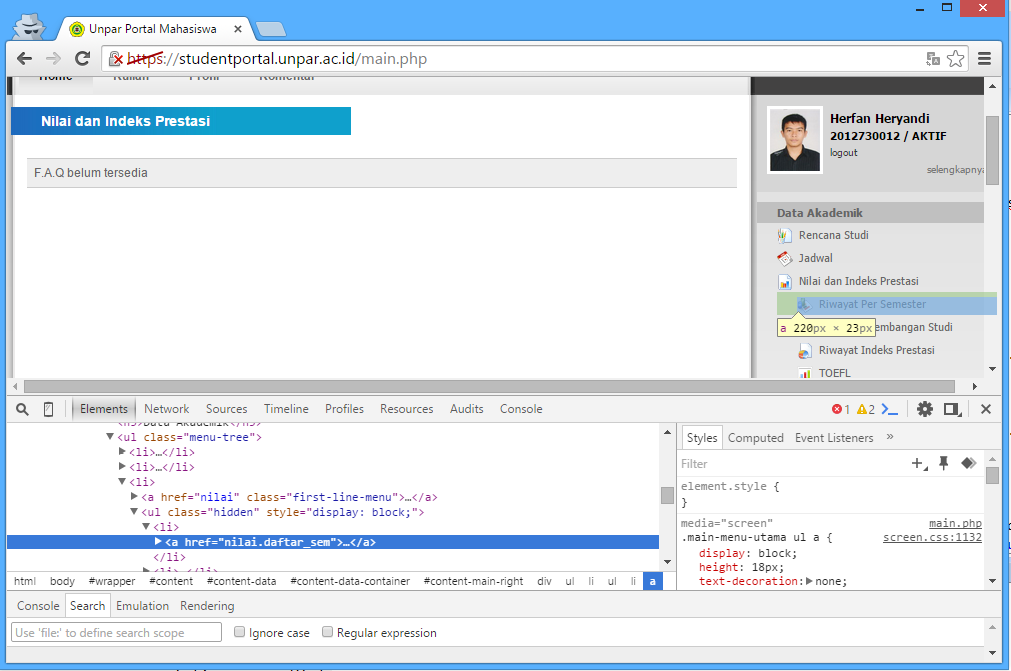
\includegraphics[scale=0.5]{Gambar/case-nilai-menu}
			\caption{Elemen ``a'' dengan teks ``Riwayat Per Semester'' pada Menu Nilai dan Indeks Prestasi} 
			\label{fig:3_case_nilai_menu}
		\end{figure}
		\item Setelah mengklik ``Riwayat Per Semester'', mahasiswa akan diarahkan ke \url{https://studentportal.unpar.ac.id/includes/nilai.daftar_sem.php} dengan \textit{cookie} sebagai berikut:
\begin{itemize}
	\item PHPSESSID: diambil dari \textit{cookie} yang di-\textit{set} saat pengalihan ke halaman utama
\end{itemize}
		\item Halaman ``Riwayat Per Semester'' menampilkan nilai semester terkini. Jika ingin melihat nilai semester sebelumnya, mahasiswa dapat mengklik \textit{combo box} ``select\#tahun\_akd\_sec'' kemudian memilih ``option'' yang diinginkan atau ``Seluruh Tahun Akademik'' untuk melihat nilai seluruh semester (Gambar \ref{fig:3_case_nilai_pilih}).
		
		\begin{figure}[H]
			\centering
			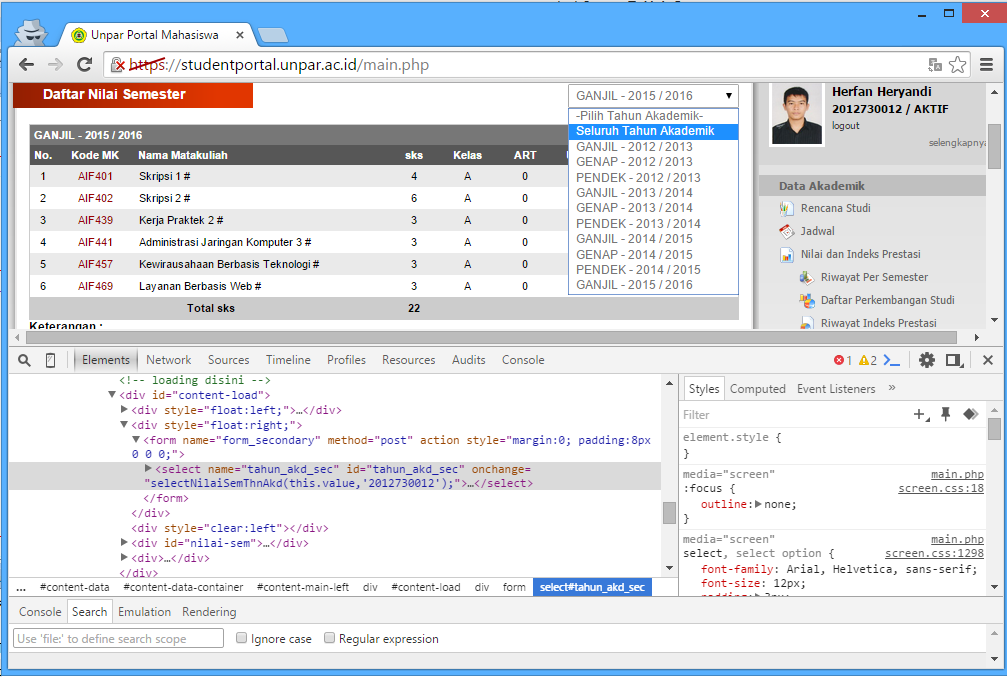
\includegraphics[scale=0.5]{Gambar/case-nilai-pilih}
			\caption{\textit{Combo Box} ``select\#tahun\_akd\_sec'' pada Halaman Riwayat Per Semester} 
			\label{fig:3_case_nilai_pilih}
		\end{figure}
		
		\item  Setelah memilih ``option'', mahasiswa akan dibawa ke \url{https://studentportal.unpar.ac.id/includes/nilai.sem.php} (Gambar \ref{fig:3_case_nilai}) dengan \textit{cookie} PHPSESSID dan mengandung \textit{form data}:
		\begin{itemize}
			\item npm: diperoleh dari NPM mahasiswa
			\item thn\_akd: berisi tahun akademik semester atau berisi ``ALL'' jika memilih ``Seluruh Tahun Akademik''
			\item sem\_akd: berisi semester akademik dalam angka (1: ganjil, 2: genap, 4: pendek) atau tidak didefinisikan jika memilih ``Seluruh Tahun Akademik''
		\end{itemize}
		
		\begin{figure}[H]
			\centering
			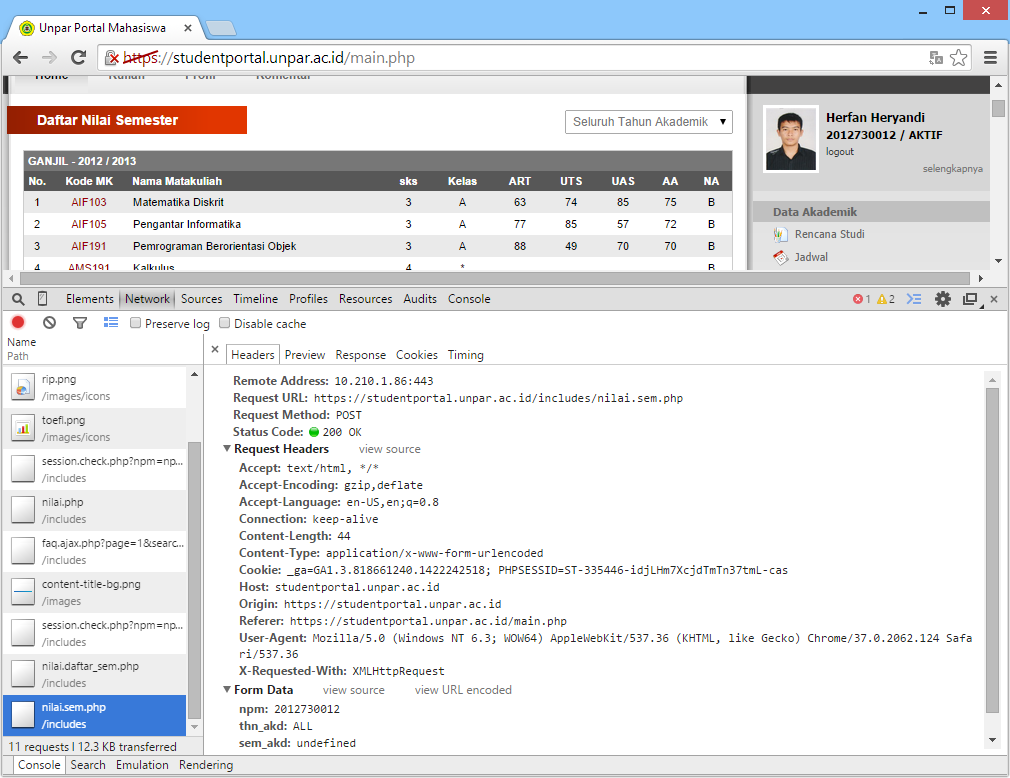
\includegraphics[scale=0.5]{Gambar/case-nilai}
			\caption{\textit{Form Data} pada pengiriman Nilai Seluruh Tahun Akademik} 
			\label{fig:3_case_nilai}
		\end{figure}
\end{enumerate}

\subsection{Kasus Jadwal}
Di halaman utama Portal Akademik Mahasiswa, mahasiswa dapat melihat jadwal dengan cara:
\begin{enumerate}
	\item Mengklik ``a.first-line-menu'' dengan teks ``Jadwal'' 
	\item Setelah diklik, akan muncul list ``ul.hidden'', kemudian mahasiswa harus mengklik elemen ``a'' dengan teks ``Kuliah, UTS dan UAS''(Gambar \ref{fig:3_case_jadwal_menu})
	\begin{figure}[H]
			\centering
			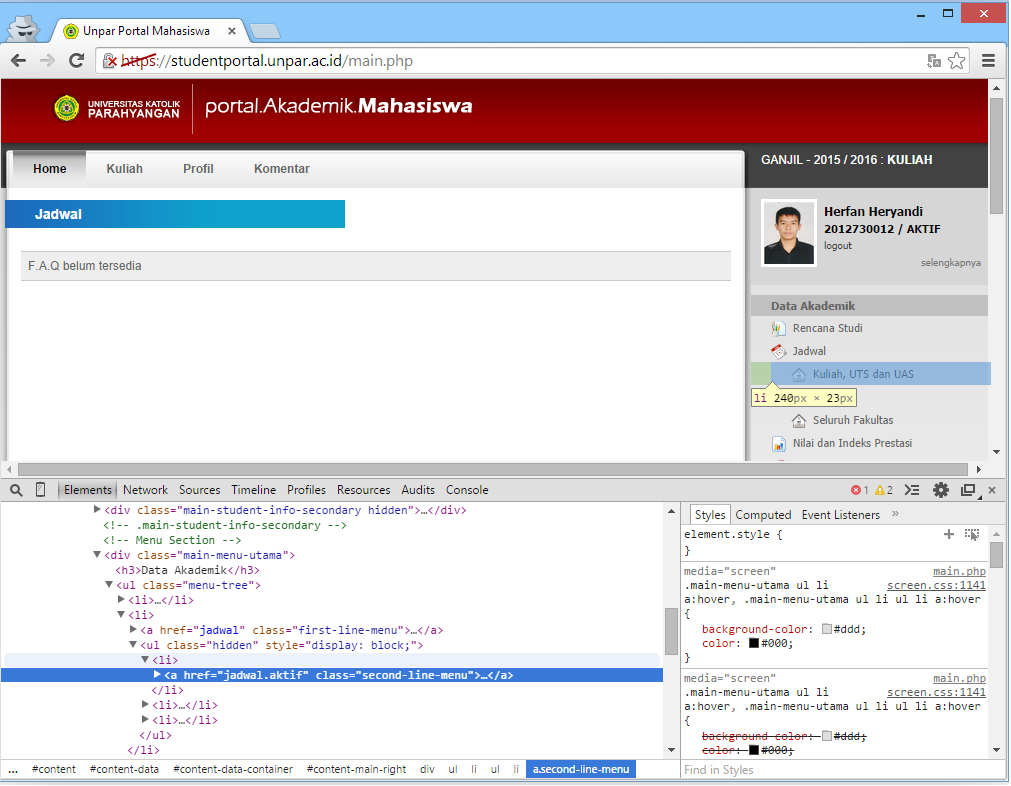
\includegraphics[scale=0.5]{Gambar/case-jadwal-menu}
			\caption{Elemen ``a'' dengan teks ``Kuliah, UTS dan UAS'' pada Menu Jadwal} 
			\label{fig:3_case_jadwal_menu}
		\end{figure}
		\item Setelah mengklik ``Kuliah, UTS dan UAS'', mahasiswa akan diarahkan ke \url{https://studentportal.unpar.ac.id/includes/jadwal.aktif.php} dengan \textit{cookie} sebagai berikut:
\begin{itemize}
	\item PHPSESSID: diambil dari \textit{cookie} yang di-\textit{set} saat pengalihan ke halaman utama
\end{itemize}
\item Halaman ``Kuliah, UTS dan UAS'' menampilkan jadwal kuliah, UTS, dan UAS semester terkini. Jika ingin melihat jadwal semester sebelumnya, mahasiswa dapat mengklik \textit{combo box} ``select\#tahun\_akd\_sec'' kemudian memilih ``option'' yang diinginkan (Gambar \ref{fig:3_case_jadwal_pilih}).
		
		\begin{figure}[H]
			\centering
			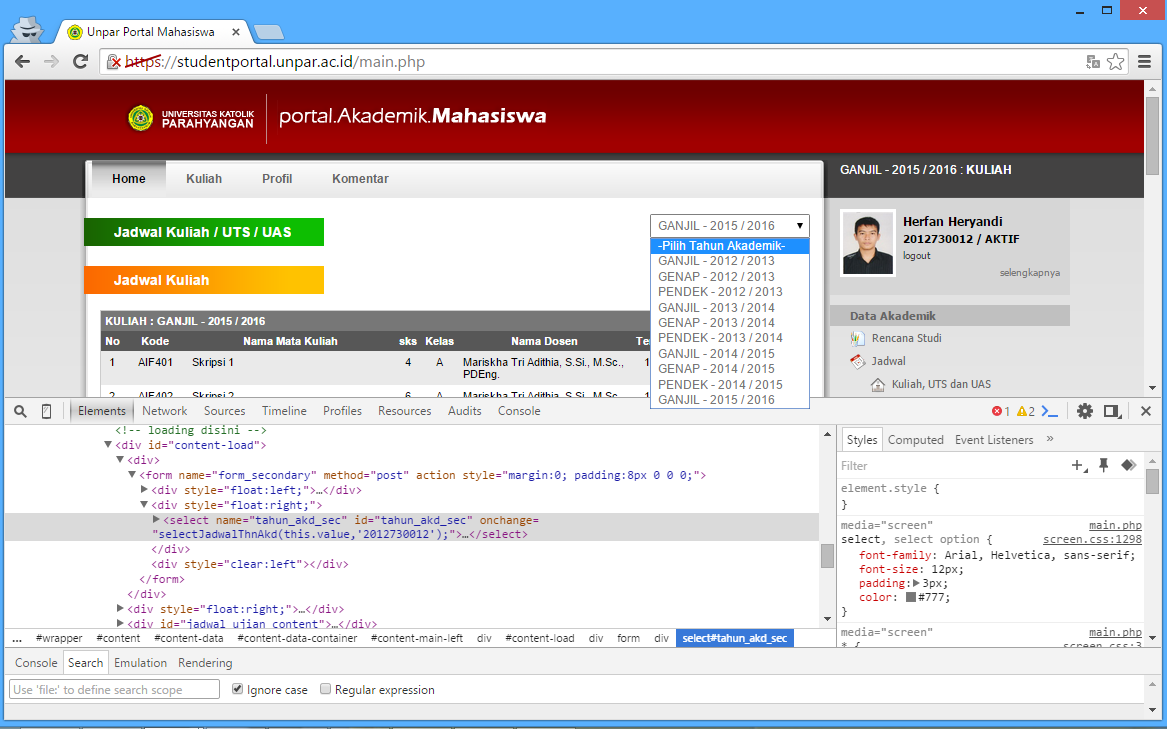
\includegraphics[scale=0.5]{Gambar/case-jadwal-pilih}
			\caption{Combo Box ``select\#tahun\_akd\_sec'' pada Halaman Jadwal Kuliah, UTS, dan UAS} 
			\label{fig:3_case_jadwal_pilih}
		\end{figure}
		
		\item  Setelah memilih ``option'', mahasiswa akan ditampilkan jawaban dari \url{https://studentportal.unpar.ac.id/includes/jadwal.kuliah.php} dan \url{https://studentportal.unpar.ac.id/includes/jadwal.ujian.php} (Gambar \ref{fig:3_case_jadwal}) dengan \textit{cookie} PHPSESSID dan mengandung \textit{form data}:
		\begin{itemize}
			\item npm: diperoleh dari NPM mahasiswa
			\item thn\_akd: berisi tahun akademik semester 
			\item sem\_akd: berisi semester akademik dalam angka (1: ganjil, 2: genap, 4: pendek) 
		\end{itemize}
		
		\begin{figure}[H]
			\centering
			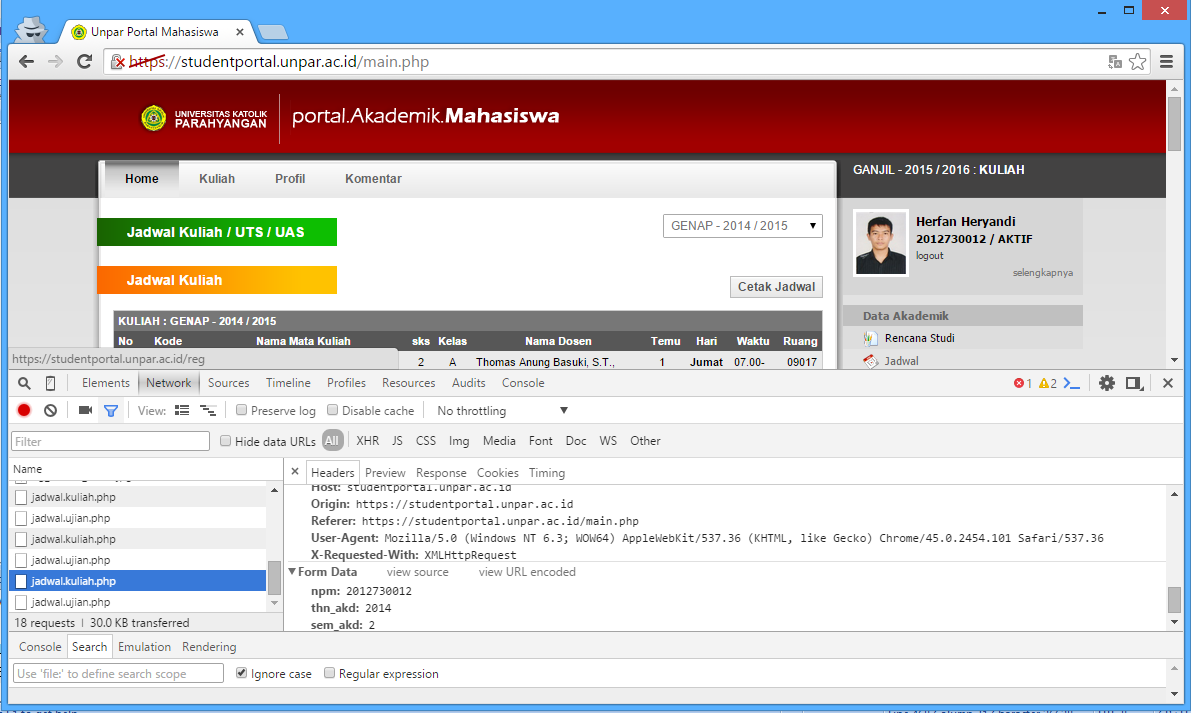
\includegraphics[scale=0.5]{Gambar/case-jadwal}
			\caption{\textit{Form Data} pada pengiriman Jadwal Kuliah dan Ujian} 
			\label{fig:3_case_jadwal}
		\end{figure}
		
\end{enumerate}

Mahasiswa juga dapat melihat jadwal seluruh fakultas dengan cara:
\begin{enumerate}
	\item Mengklik ``a.second-line-menu'' dengan teks ``Seluruh Fakultas'' pada \textit{list} ``ul.hidden'' (Gambar \ref{fig:3_case_jadwal_seluruh})
	\begin{figure}[H]
			\centering
			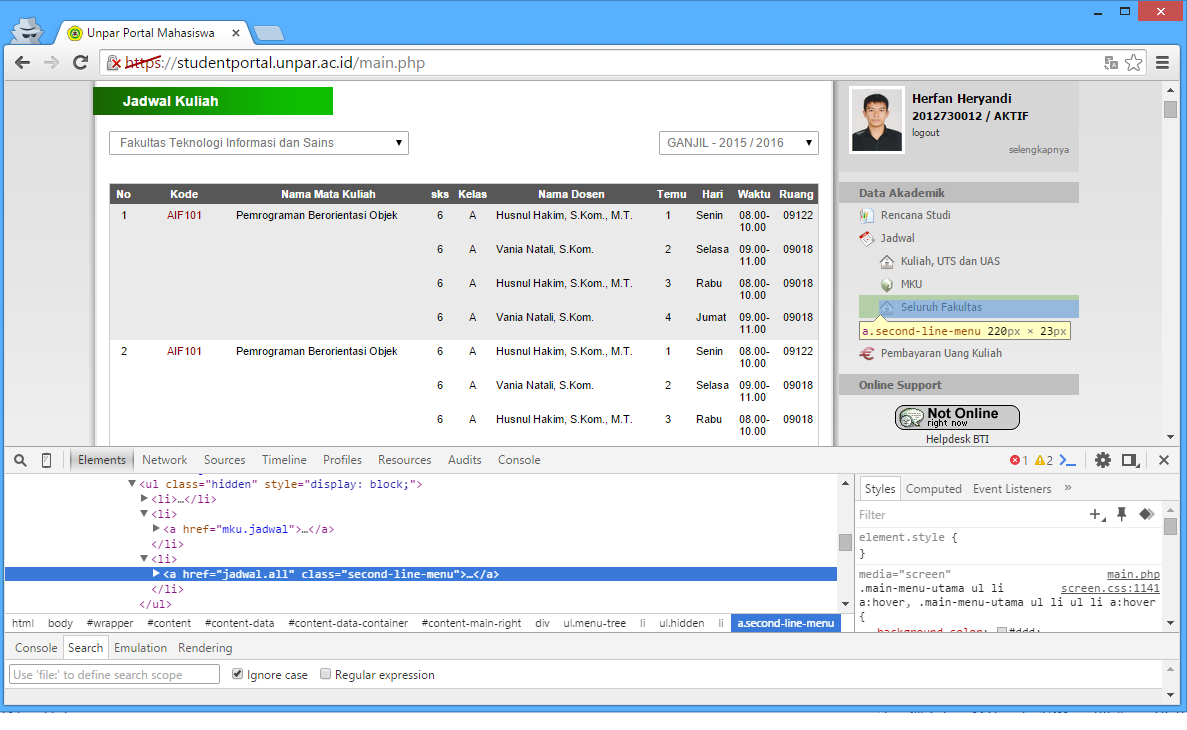
\includegraphics[scale=0.5]{Gambar/case-jadwal-seluruh}
			\caption{Elemen ``a'' dengan teks ``Seluruh Fakultas'' pada Menu Jadwal} 
			\label{fig:3_case_jadwal_seluruh}
		\end{figure}
	\item Setelah diklik, mahasiswa akan diarahkan ke \url{https://studentportal.unpar.ac.id/includes/jadwal.all.php} dengan \textit{cookie} sebagai berikut:
\begin{itemize}
	\item PHPSESSID: diambil dari \textit{cookie} yang di-\textit{set} saat pengalihan ke halaman utama
\end{itemize}
		\item Halaman ``Seluruh Fakultas'' menampilkan seluruh jadwal semester terkini pada fakultas tempat mahasiswa menempuh studi. Jika ingin melihat jadwal semester sebelumnya, mahasiswa dapat mengklik \textit{combo box} ``select\#tahun\_akd\_sec'' kemudian memilih ``option'' yang diinginkan. Jika ingin melihat jadwal fakultas lain, mahasiswa dapat mengklik \textit{combo box} ``select\#jadwal\_all\_ps'' kemudian memilih ``option'' fakultas yang diinginkan (Gambar \ref{fig:3_case_jadwal_pilihfak}).
		\begin{figure}[H]
			\centering
			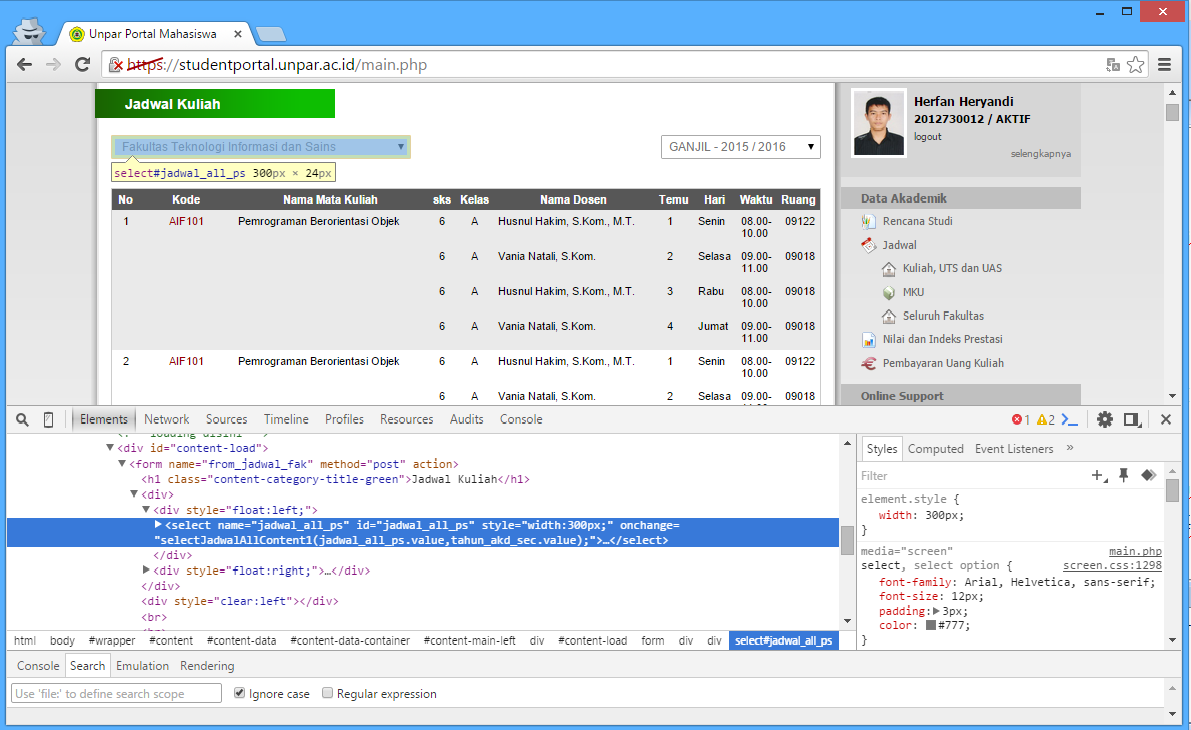
\includegraphics[scale=0.5]{Gambar/case-jadwal-pilihfak}
			\caption{Combo Box ``select\#jadwal\_all\_ps'' pada Halaman Jadwal Seluruh Fakultas} 
			\label{fig:3_case_jadwal_pilihfak}
		\end{figure}
		\item  Setelah memilih ``option'', mahasiswa akan dibawa ke \url{https://studentportal.unpar.ac.id/includes/jadwal.all.content.php}(Gambar \ref{fig:3_case_jadwal_fakultas}) dengan \textit{cookie} PHPSESSID dan mengandung \textit{query string parameter}:
		\begin{itemize}
			\item kode\_fak: berisi kode fakultas 
			\item thn\_akd: berisi tahun akademik semester 
			\item sem\_akd: berisi semester akademik dalam angka (1: ganjil, 2: genap, 4: pendek) 
		\end{itemize}
		
		\begin{figure}[H]
			\centering
			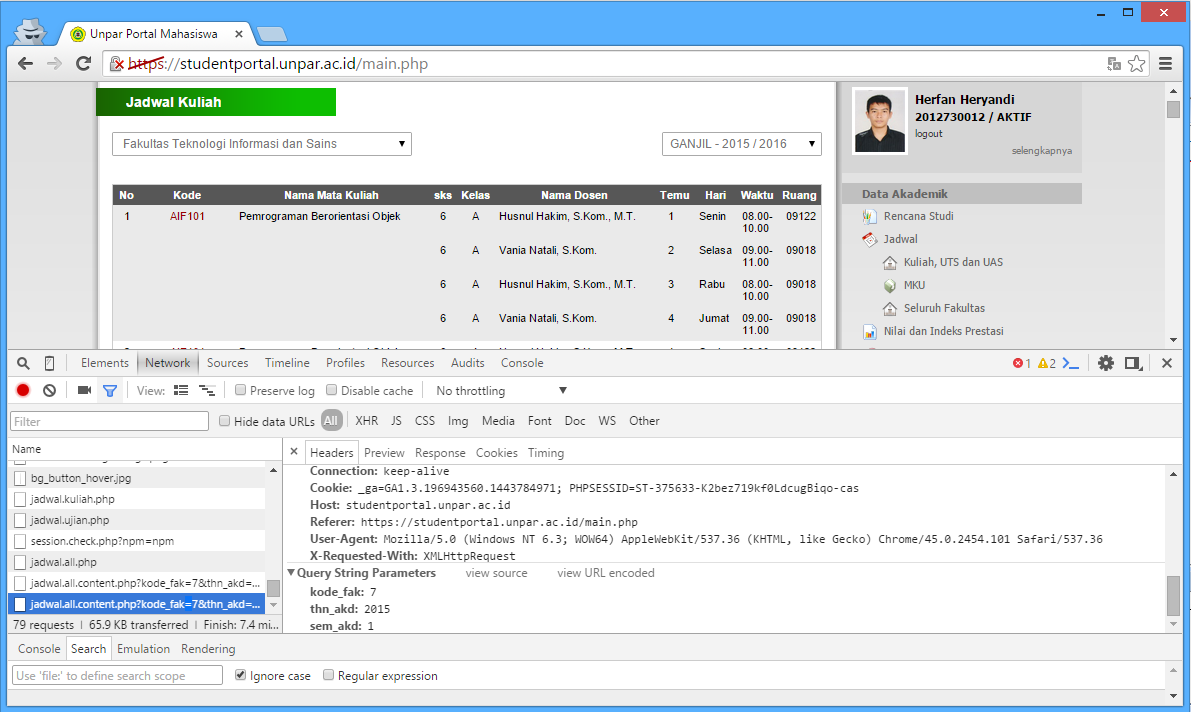
\includegraphics[scale=0.5]{Gambar/case-jadwal-fakultas}
			\caption{\textit{Form Data} pada pengiriman Jadwal Seluruh Fakultas} 
			\label{fig:3_case_jadwal_fakultas}
		\end{figure}
\end{enumerate}

\subsection{Kasus \textit{Logout}}
Mahasiswa dapat melakukan \textit{logout} dengan cara:
\begin{enumerate}
	\item Mengklik ``a'' dengan teks ``logout'' pada bagian identitas portal (Gambar \ref{fig:3_case_logout_link})
	\begin{figure}[H]
			\centering
			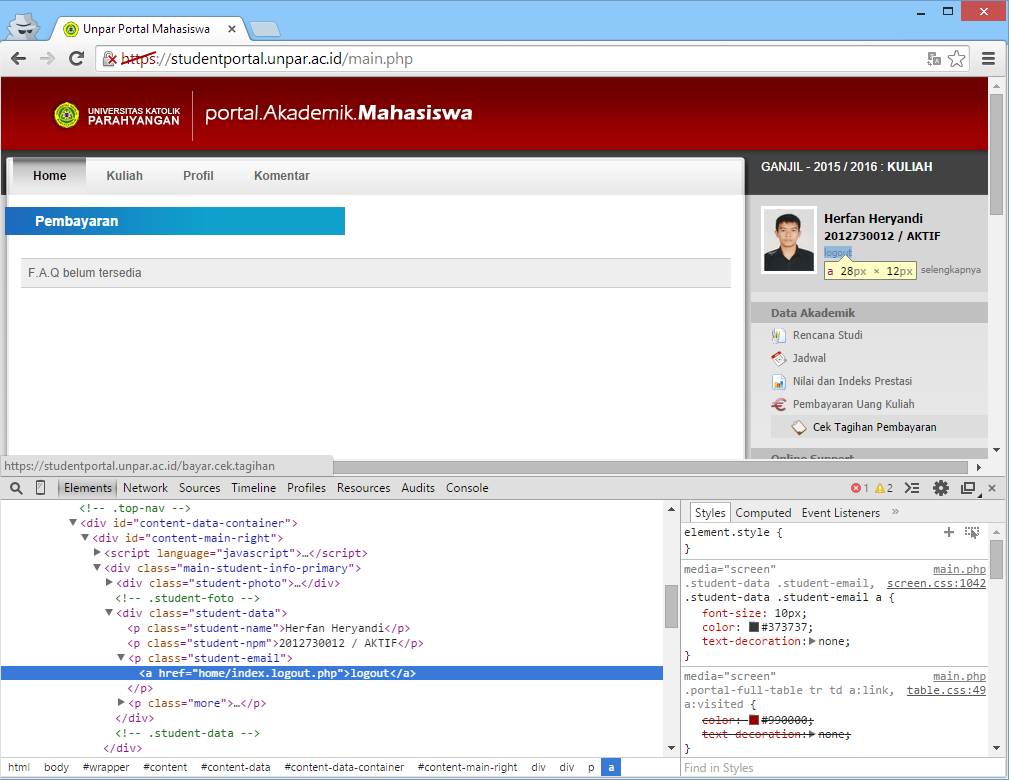
\includegraphics[scale=0.5]{Gambar/case-logout-link}
			\caption{Elemen ``a'' dengan teks ``logout'' pada Identitas Portal} 
			\label{fig:3_case_logout_link}
		\end{figure}
	\item Setelah diklik, mahasiswa akan diarahkan ke \url{https://studentportal.unpar.ac.id/home/index.logout.php} dengan \textit{cookie} sebagai berikut:
		\begin{itemize}
			\item PHPSESSID: diambil dari \textit{cookie} yang di-\textit{set} saat pengalihan ke halaman utama
		\end{itemize} 
	\item Kemudian dilakukan pengalihan ke \url{https://cas.unpar.ac.id/logout?service=https\%3A\%2F\%2Fstudentportal.unpar.ac.id} lalu mengadaluarsakan \textit{cookie} CASTGC dan CASPRIVACY yang sebelumnya di-\textit{set} saat pengalihan ke halaman utama (Gambar \ref{fig:3_case_logout_expires}) 
			\begin{figure}[H]
				\centering
				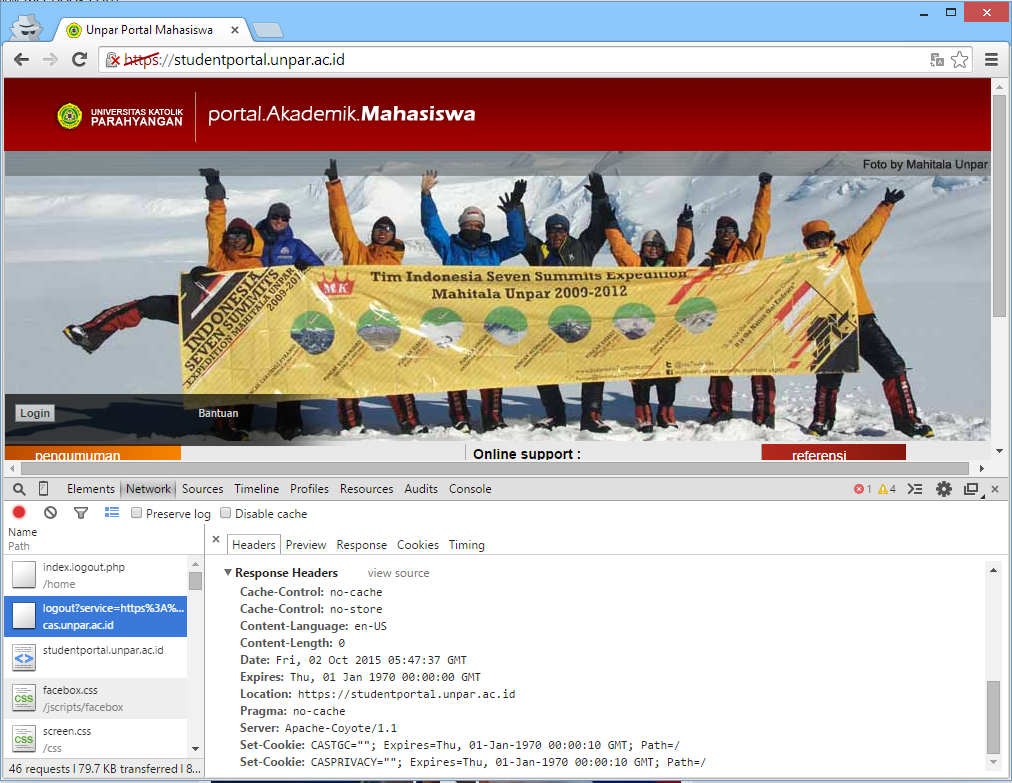
\includegraphics[scale=0.5]{Gambar/case-logout-expires}
				\caption{Pengadaluarsaan Cookie CASTGC dan CASPRIVACY} 
				\label{fig:3_case_logout_expires}
			\end{figure}
		\item Pengalihan diakhiri di \url{https://studentportal.unpar.ac.id/} yaitu halaman depan Portal Akademik Mahasiswa (Gambar \ref{fig:3_case_logout}) 
		\begin{figure}[H]
				\centering
				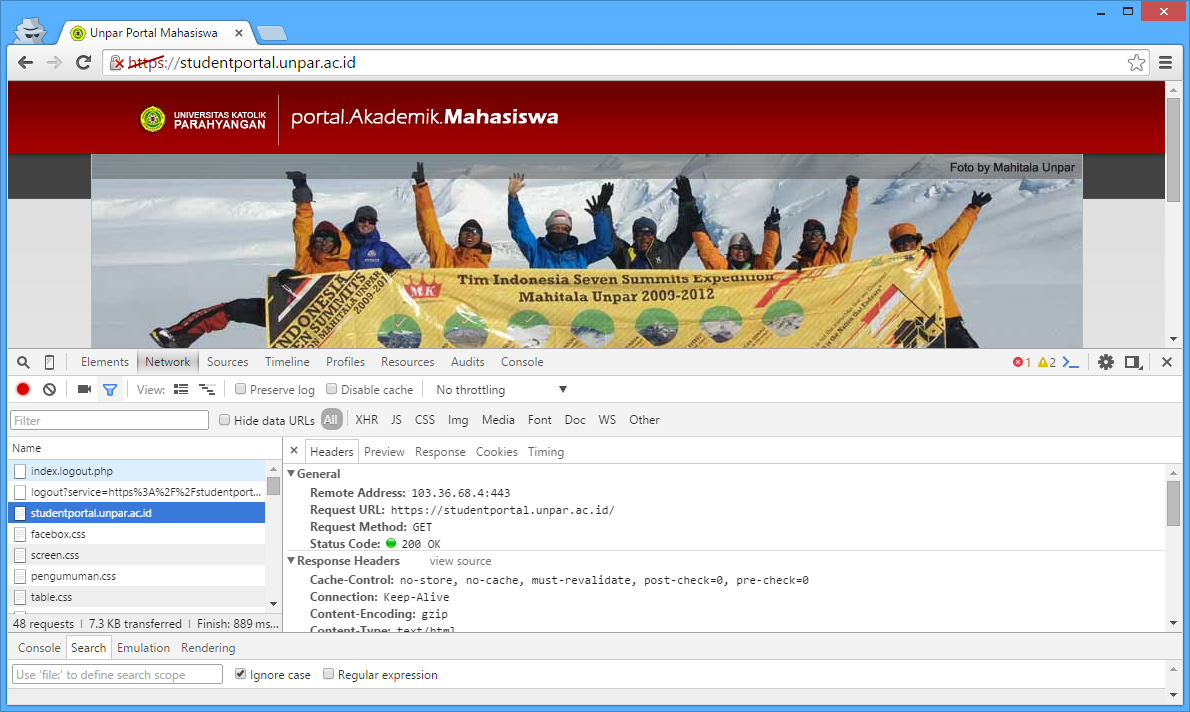
\includegraphics[scale=0.5]{Gambar/case-logout}
				\caption{Pengalihan ke Halaman Depan Portal Akademik Mahasiswa} 
				\label{fig:3_case_logout}
			\end{figure}
\end{enumerate}

Hasil analisis komunikasi Portal Akademik Mahasiswa akan digunakan untuk membangun koneksi yang akan diimplementasikan menggunakan jsoup. Berdasarkan hasil analisis tersebut, terdapat tiga hal yang perlu diperhatikan antara lain:
	\begin{itemize}
	\item Perpindahan halaman \\
		Saat pengguna melakukan suatu aksi seperti klik dan memilih \textit{option}, Portal Akademik Mahasiswa akan mengarahkan pengguna ke suatu halaman. Alamat dari halaman tersebut perlu diketahui untuk koneksi jsoup. Metode pengirimannya juga perlu diketahui. Dari seluruh halaman yang dianalisis, metode pengirimannya adalah \texttt{GET} kecuali halaman \textit{login} CAS UNPAR yang menggunakan metode POST.
	\item\textit{Cookie} \\
		Hal yang harus diperhatikan dalam penggunaan \textit{cookie} yaitu kapan suatu \textit{cookie} di-\textit{set} dan kapan \textit{cookie} tersebut dikirimkan. Jika suatu halaman memerlukan \textit{cookie} saat membangun koneksi, maka perlu diketahui kapan \textit{cookie} tersebut di-\textit{set} sehingga \textit{cookie} tersebut bisa diperoleh menggunakan jsoup. Pengiriman \textit{cookie} tersebut akan diimplementasikan dengan jsoup saat membangun koneksi ke suatu halaman yang memerlukan \textit{cookie} tersebut.
	\item Parameter\\
	Saat berpindah halaman, terkadang halaman tersebut membutuhkan parameter data. Dalam membangun koneksi, jsoup memerlukan juga memerlukan parameter data, karena itu perlu diketahui parameter data apa saja yang harus dilewatkan saat menuju suatu halaman.
\end{itemize}

\section{Analisis Arsitektur Informatika Student Portal}
Arsitektur Informatika Student Portal dapat dilihat pada Gambar \ref{fig:3_ars_portal}. \textit{Client} dapat mengakses Portal Akademik Mahasiswa dan Informatika Student Portal untuk mendapatkan informasi akademik. Namun saat mengakses Informatika Student Portal, \textit{client} akan diberikan data akademik dengan fitur-fitur yang berbeda. Saat \textit{client} mengakses Informatika Student Portal, Informatika Student Portal akan mengambil data dari Portal Akademik Mahasiswa. Data yang telah diambil akan diolah kemudian ditampilkan kepada \textit{client}.

		\begin{figure}[H]
			\centering
			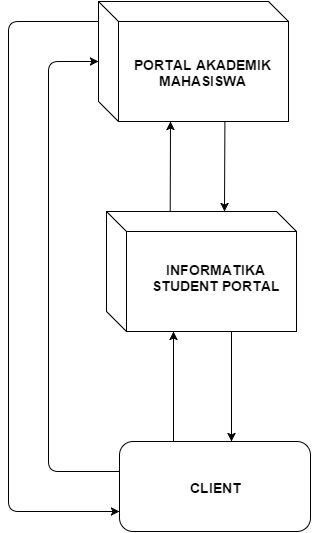
\includegraphics[scale=0.5]{Gambar/arsitekturIFPortal}
			\caption{Arsitektur Informatika Student Portal} 
			\label{fig:3_ars_portal}
		\end{figure}
		
\section{Analisis \textit{Use Case}}
\subsection{Diagram \textit{Use Case}}
Diagram \textit{use case} pada perangkat lunak yang akan dibangun hanya mengandung satu aktor, yaitu mahasiswa. Diagram \textit{use case} dapat dilihat pada gambar \ref{fig:3_usecase_diagram}. 
		\begin{figure}[H]
			\centering
			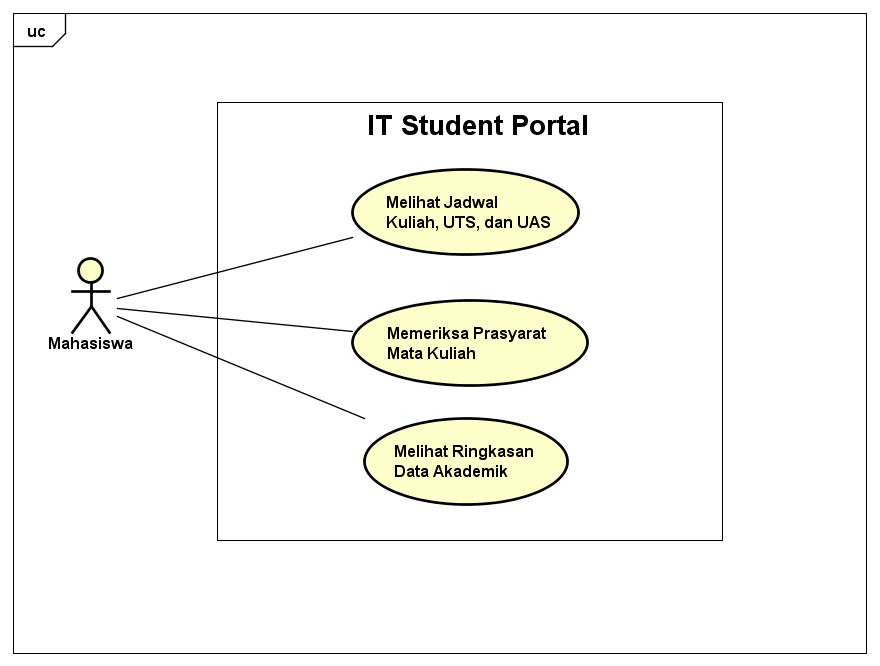
\includegraphics[scale=0.5]{Gambar/usecase-diagram}
			\caption{Diagram \textit{Use Case} Informatika Student Portal} 
			\label{fig:3_usecase_diagram}
		\end{figure}
Berdasarkan hasil analisis pada subbab \ref{sec:kebutuhan}, dari lima fitur yang akan dibuat, dibentuk tiga \textit{use case} antara lain:
\begin{itemize}
	\item \textbf{Memeriksa Prasyarat Mata Kuliah}, mahasiswa dapat memeriksa mata kuliah yang dibuka pada semester terkini apakah memenuhi prasyarat atau tidak. 
	\item \textbf{Melihat Jadwal Kuliah}, mahasiswa dapat melihat jadwal kuliah yang sudah tersusun dan terurut berdasarkan hari.
	\item \textbf{Melihat Ringkasan Data Akademik}, mahasiswa dapat melihat data mengenai mata kuliah apa saja yang sudah lulus beserta jenis mata kuliahnya(wajib, pilihan, atau pilihan wajib), sisa SKS untuk mencapai kelulusan, dan mata kuliah wajib yang belum ditempuh. Mahasiswa juga dapat melihat IPS dan IPK yang berubah berdasarkan riwayat nilai.
\end{itemize}

\subsection{Skenario \textit{Use Case}}

\begin{enumerate}
	\item \textbf{Memeriksa Prasyarat Mata Kuliah}
		\begin{itemize}
			\item Nama: Memeriksa prasyarat mata kuliah
			\item Aktor: Mahasiswa
			\item Deskripsi: Memeriksa prasyarat mata kuliah yang dibuka pada semester terkini
			\item Kondisi awal: Mahasiswa telah \textit{login}
			\item Kondisi akhir: Halaman prasyarat mata kuliah ditampilkan dan berisi mata kuliah yang dibuka pada semester terkini beserta status prasyaratnya
			\item Skenario utama: \\ \\
				\begin{tabular}{|p{0.5cm} |p{6cm}| p{6cm}|}
						\hline
							No 	& Aksi Aktor & Reaksi Sistem \\ \hline
							1 	& Mahasiswa memilih menu prasyarat mata kuliah. 	&	Sistem mendapatkan data mahasiswa kemudian menampilkan halaman prasyarat mata kuliah \\ \hline 
						\end{tabular} 
			\item Eksepsi: Mahasiswa sedang menempuh semester 1
		\end{itemize}
		
	\item \textbf{Melihat Jadwal Kuliah}
		\begin{itemize}
			\item Nama: Melihat jadwal kuliah
			\item Aktor: Mahasiswa
			\item Deskripsi: Melihat jadwal kuliah yang sudah tersusun dan terurut berdasarkan hari
			\item Kondisi awal: Mahasiswa telah \textit{login}
			\item Kondisi akhir: Halaman jadwal ditampilkan dan berisi jadwal kuliah yang sudah tersusun dan terurut berdasarkan hari te
			\item Skenario utama: \\ \\
				\begin{tabular}{|p{0.5cm} |p{6cm}| p{6cm}|}
						\hline
							No 	& Aksi Aktor & Reaksi Sistem \\ \hline
							1 	& Mahasiswa memilih menu jadwal. 	&	Sistem menyusun dan mengurutkan jadwal mahasiswa berdasarkan hari kemudian menampilkan halaman jadwal \\ \hline 
						\end{tabular} 
			\item Eksepsi: Mahasiswa sedang cuti studi atau jadwal kuliah belum keluar
		\end{itemize}
		
	\item \textbf{Melihat Ringkasan Data Akademik}
		\begin{itemize}
			\item Nama: Melihat ringkasan data akademik
			\item Aktor: Mahasiswa
			\item Deskripsi: melihat data mengenai mata kuliah apa saja yang sudah lulus beserta jenis mata kuliahnya(wajib, pilihan, atau pilihan wajib), sisa SKS untuk mencapai kelulusan, dan mata kuliah wajib yang belum ditempuh. Mahasiswa juga dapat melihat IPS dan IPK yang berubah berdasarkan riwayat nilai
			\item Kondisi awal: Mahasiswa telah \textit{login}
			\item Kondisi akhir: Halaman jadwal ditampilkan dan berisi jadwal ringkasan data akademik
			\item Skenario utama: \\ \\
			\begin{tabular}{|p{0.5cm} |p{6cm}| p{6cm}|}
						\hline
							No 	& Aksi Aktor & Reaksi Sistem \\ \hline
							1 	& Mahasiswa memilih menu ringkasan data akademik. 	&	Sistem meringkas data kademik mahasiswa kemudian menampilkan halaman ringkasan data akademik \\ \hline 
						\end{tabular} 
			\item Eksepsi: Mahasiswa sedang menempuh semester 1
		\end{itemize}
\end{enumerate}

\section{Analisis Kelas}
\label{sec:analisis_kelas}
Diagram kelas analisis untuk Informatika Student Portal ditunjukkan pada gambar \ref{fig:3_class_diagram}.
	\begin{figure}[H]
			\centering
			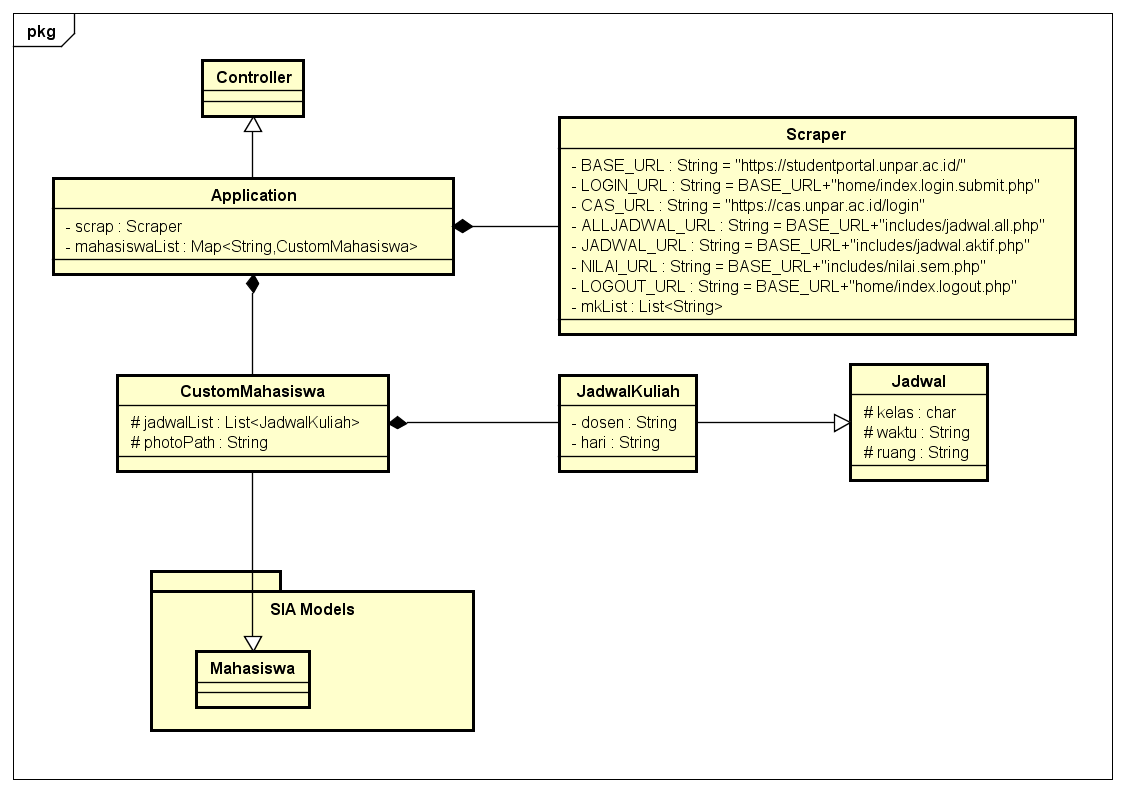
\includegraphics[scale=0.5]{Gambar/class-diagram}
			\caption{Diagram Kelas Analisis Informatika Student Portal} 
			\label{fig:3_class_diagram}
		\end{figure}
Kelas-kelas dari \textit{package} SIA Models telah dibahas pada subbab \ref{sec:siamodels}. Sedangkan penjelasan dari kelas-kelas lainnya sebagai berikut:
\begin{enumerate}
	\item Controller\\
	Kelas ini merupakan kelas yang sudah disediakan oleh Play Framework. Turunan dari kelas ini akan berperan sebagai \textit{controller}.
	\item Application\\
	Kelas ini merupakan \textit{controller} pada Informatika Student Portal yang berfungsi untuk menghubungkan \textit{model} dengan \textit{view}. 
	\item Scraper\\
	Kelas ini merupakan kelas yang mengimplementasikan \textit{web scraping} menggunakan \textit{library} jsoup. Kelas ini digunakan untuk memperoleh data dari Portal Akademik Mahasiswa kemudian menghubungkannya ke dalam SIA Models. Data-data yang sudah dihubungkan dengan SIA Models akan ditampilkan ke \textit{view} melalui kelas \texttt{Application}.
	\item CustomMahasiswa\\
	Kelas ini turunan dari kelas Mahasiswa pada SIA Models. Kelas ini merepresentasikan mahasiswa yang memiliki jadwal kuliah dan URL foto profil pada Portal Akademik Mahasiswa.
	\item Jadwal\\
	Kelas ini merepresentasikan jadwal di UNPAR.
	\item Jadwal Kuliah\\
	Kelas ini merupakan turunan dari kelas Jadwal yang merepresentasikan jadwal kuliah di UNPAR.
\end{enumerate}
		}{}
\ifdefstring{\vbabd}{1}{\chapter{Perancangan}
\label{chap:perancangan}}{}
\ifdefstring{\vbabe}{1}{\chapter{Implementasi dan Pengujian}
\label{chap:implementasiPengujian}

\section{Implementasi}
\label{sec:implementasi}

\subsection{Lingkungan Implementasi}
		\label{sec:lingkungan_implementasi}
			Implementasi perangkat lunak ini dilakukan di dua buah komputer. Implementasi pertama dilakukan pada komputer peneliti untuk keperluan pengujian fungsional. Komputer tersebut memiliki spesifikasi sebagai berikut:
				\begin{enumerate}
					\item Processor: 3.20Ghz 
					\item RAM: 4.00 GB DDR3	
					\item Sistem Operasi: Windows 8.1 Pro 64-bit 
					\item Versi Java: 1.8.0\_40
				\end{enumerate}
				Implementasi kedua dilakukan pada komputer server yang terhubung dengan jaringan FTIS untuk keperluan pengujian eksperimental. Komputer tersebut memiliki spesifikasi sebagai berikut:
				\begin{enumerate}
					\item Processor: 2.40Ghz 
					\item RAM: 4.00 GB DDR3	
					\item Sistem Operasi: Ubuntu server amd-64 
					\item Versi Java: 1.8.0\_85
				\end{enumerate}

\subsection{Hasil Implementasi}
				
\section{Pengujian}
			\subsection{Pengujian Fungsional} 
			Pengujian fungsional dilakukan untuk mengetahui kesesuaian reaksi perangkat lunak dengan reaksi yang diharapkan berdasarkan aksi pengguna terhadap perangkat lunak. Ada tujuh tes kasus yang diujikan, dan detail serta hasilnya dapat dilihat di tabel \ref{table:hasilFungsional}.
			
			\begin{table}[H]
			\centering
			\caption{Tabel Pengujian Fungsional}
				\begin{tabular}{|p{0.5cm}| p{3.5cm}| p{7cm}| p{2.25cm}|} \hline
				No.	&	Aksi Pengguna	&	Reaksi yang diharapkan	&	Reaksi Perangkat Lunak \\ \hline
				1.	&	Pengguna menjalankan aplikasi	&	Halaman \textit{login} akan ditampilkan	&	sesuai	\\ \hline
				2.	&	Pengguna memasukkan \textit{email} dan \textit{password}	&	Jika \textit{email} dan \textit{password}	sesuai, pengguna akan diarahkan ke halaman utama. & sesuai, namun foto profil tidak muncul jika belum validasi sertifikat SSL UNPAR\\ \hline
					&	&	Jika \textit{email} yang dimasukkan bukan \textit{email} \textit{student} UNPAR, akan ditampilkan pesan ``Email tidak valid''&	sesuai	\\ \hline
					&	&	Jika \textit{email} yang dimasukkan bukan \textit{email} mahasiswa teknik informatika, akan ditampilkan pesan ``Maaf, Anda bukan mahasiswa teknik informatika''	&	sesuai	\\ \hline
					&	&	Jika \textit{email} dan \textit{password} tidak sesuai atau mahasiswa bukan mahasiswa aktif, akan ditampilkan pesan ``Password yang Anda masukkan salah atau Anda bukan mahasiswa aktif''	&	sesuai	\\ \hline
				3.	&	Pengguna memilih menu ``Prasyarat Mata Kuliah'' &	Jika pengguna belum memiliki riwayat nilai(masih menempuh semester 1), akan ditampilkan pesan ``PRASYARAT BELUM TERSEDIA''	&	sesuai	\\ \hline
					&	&	Jika pengguna sudah memiliki riwayat nilai	akan ditampilkan tabel prasyarat mata kuliah beserta status pengambilannya &	sesuai	\\ \hline
				4.	&	Pengguna memilih menu ``Jadwal Kuliah'' &	Jika pengguna belum melakukan FRS, cuti studi, atau jadwal kuliah pengguna belum tersedia, akan ditampilkan pesan ``JADWAL KULIAH BELUM TERSEDIA''	&	sesuai	\\ \hline
					&	&	Jika jadwal kuliah pengguna sudah tersedia, akan ditampilkan jadwal kuliah dalam bentuk kalendar yang sudah diurutkan berdasarkan hari &	sesuai	\\ \hline
				5.	&	Pengguna memilih menu ``Data Akademik'' &	Jika pengguna belum memiliki riwayat nilai(masih menempuh semester 1), akan ditampilkan pesan ``DATA AKADEMIK BELUM TERSEDIA'' &	sesuai	\\ \hline
					&	&	Jika pengguna sudah memiliki riwayat nilai, akan ditampilkan ringkasan data akademik mahasiswa berupa IPS semester terakhir, IPK, SKS lulus, sisa SKS kelulusan, dan ringkasan data mengenai mata kuliah pilihan wajib &	sesuai	\\ \hline
				6.	&	Pengguna memilih tombol \textit{logout}	&	Pengguna akan diarahkan kembali ke halaman \textit{login} &	sesuai	\\ \hline
				7.	& Dua pengguna menggunakan aplikasi secara bersamaan	&	Pengguna dapat menggunakan aplikasi dengan akun yang sesuai &	sesuai	\\ \hline
				\end{tabular}
				\label{table:hasilFungsional}
			\end{table}
			
		\subsection{Pengujian Eksperimental} 
		}{}
\ifdefstring{\vbabf}{1}{\chapter{Kesimpulan dan Saran}
\label{chap:kesimpulan_saran}

\section{Kesimpulan}
\label{sec:kesimpulan}
Dari hasil pembangunan aplikasi Informatika Student Portal, didapatkanlah kesimpulan-kesimpulan sebagai berikut:
		\begin{enumerate}
			\item Fitur-fitur yang dibuat untuk Informatika Student Portal antara lain prasyarat mata kuliah, jadwal kuliah yang tersusun dan terurut berdasarkan hari, data akademik berupa IPS dan IPK yang langsung berubah ketika nilai sudah muncul, sisa SKS, dan status kelulusan mata kuliah pilihan wajib, dan aplikasi yang dapat diakses dari sistem operasi manapun.
			\item Telah berhasil mengimplementasikan \textit{web scraping} menggunakan \textit{library} jsoup. Dengan \textit{library} jsoup, data dari Portal Akademik Mahasiswa dapat diperoleh secara langsung.
			\item Aplikasi Informatika Student Portal telah berhasil dibangun dengan menggunakan Play Framework. Selain itu, aplikasi Informatika Student Portal juga memperoleh data dari Portal Akademik Mahasiswa secara langsung menggunakan \textit{library} jsoup kemudian mengolah data tersebut dengan bantuan SIA Models. 
		\end{enumerate}

\section{Saran}
\label{sec:saran}
Dari hasil penelitian termasuk kesimpulan yang didapat, berikut adalah beberapa saran untuk pengembangan:
	\begin{enumerate}
		\item Penelitian ini memanfaatkan SIA Model terutama \textit{package} \texttt{id.ac.unpar.siamodels.matakuliah} yang berisi aturan mengenai prasyarat mata kuliah. Aturan-aturan tersebut dapat berubah suatu saat. Oleh karena itu, sebaiknya SIA Models dipisahkan dari \textit{project} Play sehingga jika terjadi perubahan aturan pada SIA Models, tidak perlu dilakukan perubahan pada \textit{project} yang dapat mengakibatkan . 
		\item Dalam pengembangan berikutnya, perlu diperhatikan data dari mahasiswa yang pernah melakukan transfer studi. Jika memungkinkan, sebaiknya dianalisis langsung dari akun Portal Akademik Mahasiswa milik mahasiswa tersebut agar dapat mengambil data yang sesuai. Saat ini, aplikasi mengambil data langsung dari halaman riwayat nilai Portal Akademik Mahasiwa. Terdapat halaman lain yang memuat nilai mahasiswa pada Portal Akademik Mahasiswa yaitu halaman Daftar Perkembangan Studi (DPS). Sebaiknya pengambilan nilai dilakukan pada halaman DPS.
		\item Saat ini, apliaksi berjalan pada port 9000 dan tidak dijalankan secara otomatis saat server mulai berjalan. Sebaiknya aplikasi dapat langsung berjalan saat server mulai berjalan dan aplikasi juga dapat berjalan pada port 80.
		\item Aplikasi belum dapat menangani \textit{path} yang tidak terdapat pada \textit{routes} sehingga aplikasi akan memberikan pesan error jika memasuki \textit{path} tersebut. Dalam pengembangan berikutnya, path yang tidak ditemukan sebaiknya diarahkan ke halaman ``404 Not Found''.
	\end{enumerate}}{}
\ifdefstring{\vbabg}{1}{\include{Bab/bab7}}{}
\ifdefstring{\vbabh}{1}{\include{Bab/bab8}}{}
\ifdefstring{\vbabi}{1}{\include{Bab/bab9}}{}

\bibliographystyle{ieeetr}
\bibliography{pustaka}

\appendix
\apptoc

\tampillmp{\vlmp}
\ifdefstring{\vlmpa}{1}{\chapter{Kode Program}

%selalu gunakan single spacing untuk source code !!!!!
\singlespacing 
% language: bahasa dari kode program
% terdapat beberapa pilihan : Java, C, C++, PHP, Matlab, R, dll
%
% basicstyle : ukuran font untuk kode program
% terdapat beberapa pilihan : tiny, scriptsize, footnotesize, dll
%
% caption : nama yang akan ditampilkan di dokumen akhir, lihat contoh
\begin{lstlisting}[language=Java,basicstyle=\tiny,caption=Application.java]
package controllers;

import java.io.IOException;
import java.lang.instrument.Instrumentation;
import java.util.ArrayList;
import java.util.HashMap;
import java.util.List;
import java.util.Map;

import org.jsoup.Connection;
import org.jsoup.nodes.Document;

import models.display.JadwalDisplay;
import models.display.PrasyaratDisplay;
import models.display.RingkasanDisplay;
import models.id.ac.unpar.siamodels.Mahasiswa;
import models.id.ac.unpar.siamodels.MataKuliah;
import models.id.ac.unpar.siamodels.Mahasiswa.Nilai;
import models.id.ac.unpar.siamodels.MataKuliahFactory;
import models.id.ac.unpar.siamodels.Semester;
import models.id.ac.unpar.siamodels.matakuliah.interfaces.HasPrasyarat;
import models.support.CustomMahasiswa;
import models.support.JadwalKuliah;
import models.support.Scraper;
import play.*;
import play.data.DynamicForm;
import play.data.Form;
import play.mvc.*;
import views.html.*;

public class Application extends Controller {
	Scraper scrap = new Scraper();
	Map<String,CustomMahasiswa> mahasiswaList = new HashMap<String,CustomMahasiswa>();
	
    public Result index() {
    	if(session("npm")==null){
    		return ok(views.html.login.render(""));
    	}
    	else{
    		return home();
    	}
    }
    
    public Result login() {
    	if(session("npm")==null){
    		return index();
    	}
    	else{
    		return home();
    	}
    }
    
    public Result submitLogin() throws IOException{
    	String errorHtml = 
    	"<div class='alert alert-danger' role='alert'>" +
    	  "<span class='glyphicon glyphicon-exclamation-sign' aria-hidden='true'></span>"+
    	  "<span class='sr-only'>Error:</span>";
    	DynamicForm dynamicForm = Form.form().bindFromRequest();
    	String email = dynamicForm.get("email");
    	String pass = dynamicForm.get("pass");
    	if(!email.matches("[0-9]{7}+@student.unpar.ac.id")){
    		return ok(views.html.login.render(errorHtml+ "Email tidak valid" + "</div>"));
    	}
    	if(!(email.charAt(0)=='7'&&email.charAt(1)=='3')){
    		return ok(views.html.login.render(errorHtml+"Maaf, Anda bukan mahasiswa teknik informatika"+ "</div>"));
    	}
    	String npm = "20" + email.substring(2,4) + email.substring(0,2)+ "0" + email.substring(4,7);
    	CustomMahasiswa login_mhs = this.scrap.login(npm, pass);
    	if(login_mhs!=null){
    		session("npm", npm);
    		mahasiswaList.put(session("npm"), login_mhs);
    		return home();
    	}
	    else{
	    	return ok(views.html.login.render(errorHtml+"Password yang Anda masukkan salah atau Anda bukan mahasiswa aktif"+ "</div>"));
	    }
    }
    
    public Result home() {
    	if(session("npm")==null){
    		return index();
    	}
    	else{
    		return ok(views.html.home.render(mahasiswaList.get(session("npm"))));	
    	}
    }
    
    public Result prasyarat() throws IOException{
    	if(session("npm")==null){
    		return index();
    	}
    	else if(mahasiswaList.get(session("npm")).getRiwayatNilai().size()==0){
    		List<PrasyaratDisplay> table = null;
	    	String semester = scrap.getSemester();
	    	return ok(views.html.prasyarat.render(table,semester));
    	}
    	else{
	    	List<PrasyaratDisplay> table = checkPrasyarat();
	    	String semester = scrap.getSemester();
	    	return ok(views.html.prasyarat.render(table,semester));
    	}
    }
    
    public Result jadwalKuliah() throws IOException{
    	if(session("npm")==null){
    		return index();
    	}
    	else{
			JadwalDisplay table = new JadwalDisplay(mahasiswaList.get(session("npm")).getJadwalList());
			String semester = scrap.getSemester();
	    	return ok(views.html.jadwalKuliah.render(table,semester));
    	}
    }

    public Result ringkasan() throws IOException{
    	if(session("npm")==null){
    		return index();
    	}
    	else if(mahasiswaList.get(session("npm")).getRiwayatNilai().size()==0){
    		RingkasanDisplay display  = null;;
	    	return ok(views.html.ringkasan.render(display));
    	}
    	else{
    		Mahasiswa currMahasiswa = mahasiswaList.get(session("npm"));
    		RingkasanDisplay display = new RingkasanDisplay(
				String.format("%.2f", currMahasiswa.calculateIPS()), 
				String.format("%.2f", currMahasiswa.calculateIPKLulus()), 
				currMahasiswa.calculateSKSLulus()
			);
	    	List<Nilai> riwayatNilai = currMahasiswa.getRiwayatNilai();	
	    	int lastIndex = riwayatNilai.size() - 1;
			Semester semester = riwayatNilai.get(lastIndex).getSemester();
			int tahunAjaran = riwayatNilai.get(lastIndex).getTahunAjaran();
			int totalSKS = 0;
			for (int i = lastIndex; i >= 0; i--) {
				Nilai nilai = riwayatNilai.get(i);
				if (nilai.getSemester() == semester && nilai.getTahunAjaran() == tahunAjaran) {
					if (nilai.getAngkaAkhir() != null) {
						totalSKS += nilai.getMataKuliah().sks();
					}
				} else {
					break;
				}
			}

			String semTerakhir = semester +" "+tahunAjaran+"/"+(tahunAjaran+1);
	    	display.setDataSemTerakhir(semTerakhir, totalSKS);
    		String pilWajibLulus = new String();
	    	String pilWajibBelumLulus = new String();
    		for(int i=0; i<display.getPilWajib().length; i++){
	    		if( mahasiswaList.get(session("npm")).hasLulusKuliah(display.getPilWajib()[i])){
	    			pilWajibLulus += display.getPilWajib()[i]+";";
	    		}
	    		else{
	    			pilWajibBelumLulus += display.getPilWajib()[i]+";";
	    		}
	    	}
    		if(!pilWajibLulus.isEmpty()){
	    		display.setPilWajibLulus(pilWajibLulus.split(";"));
    		}
    		else{
    			display.setPilWajibLulus(new String[]{});
    		}
    		if(!pilWajibBelumLulus.isEmpty()){
	    		display.setPilWajibBelumLulus(pilWajibBelumLulus.split(";"));
    		}
    		else{
    			display.setPilWajibBelumLulus(new String[]{});
    		}
    		return ok(views.html.ringkasan.render(display));
    	}
    }
    
    public Result logout() throws IOException {
    	session().clear();
    	mahasiswaList.remove(session("npm"));
    	return index();
    }
    
    private List<PrasyaratDisplay> checkPrasyarat() throws IOException{
    	List<PrasyaratDisplay> table = new ArrayList<PrasyaratDisplay>();
    	List<MataKuliah> mkList = scrap.getMkList();
        String MATAKULIAH_REPOSITORY_PACKAGE = "models.id.ac.unpar.siamodels.matakuliah"; 
    	List<Object> mkKnown = new ArrayList<Object>(); 
    	List<MataKuliah> mkUnknown = new ArrayList<MataKuliah>(); 
        for(MataKuliah mk : mkList){
	        try {
	            Class<?> mkClass = Class.forName(MATAKULIAH_REPOSITORY_PACKAGE + "." + mk.kode());
	            Object matakuliah = mkClass.newInstance();
	            mkKnown.add(matakuliah);
	        } catch (ClassNotFoundException e) {
	        	mkUnknown.add(mk);
	        } catch (InstantiationException e) {
	                e.printStackTrace();
	        } catch (IllegalAccessException e) {
	                e.printStackTrace();
	        }           
        }
        
        for (Object mk: mkKnown) {
            if (mk instanceof HasPrasyarat) {
                List<String> reasons = new ArrayList<String>();
                ((HasPrasyarat)mk).checkPrasyarat(mahasiswaList.get(session("npm")), reasons);
                if (!reasons.isEmpty()) {
                    String status = new String();
            		for (String reason: reasons) {
            			status+=reason + ";";
                    }
                    table.add(new PrasyaratDisplay(MataKuliahFactory.createMataKuliah(mk.getClass().getSimpleName(),MataKuliahFactory.UNKNOWN_SKS,MataKuliahFactory.UNKNOWN_NAMA),status.split(";")));
                }
                else{
                    if(mahasiswaList.get(session("npm")).hasLulusKuliah(mk.getClass().getSimpleName())){
                    	table.add(new PrasyaratDisplay(MataKuliahFactory.createMataKuliah(mk.getClass().getSimpleName(),MataKuliahFactory.UNKNOWN_SKS,MataKuliahFactory.UNKNOWN_NAMA),new String[]{"sudah lulus"}));
                    }
                    else{ 
                    	table.add(new PrasyaratDisplay(MataKuliahFactory.createMataKuliah(mk.getClass().getSimpleName(),MataKuliahFactory.UNKNOWN_SKS,MataKuliahFactory.UNKNOWN_NAMA),new String[]{"memenuhi syarat"}));
                    }
                }
            }
            else{ 
            	if(mahasiswaList.get(session("npm")).hasLulusKuliah(mk.getClass().getSimpleName())){
                	table.add(new PrasyaratDisplay(MataKuliahFactory.createMataKuliah(mk.getClass().getSimpleName(),MataKuliahFactory.UNKNOWN_SKS,MataKuliahFactory.UNKNOWN_NAMA),new String[]{"sudah lulus"}));
                }
                else{ 
                	table.add(new PrasyaratDisplay(MataKuliahFactory.createMataKuliah(mk.getClass().getSimpleName(),MataKuliahFactory.UNKNOWN_SKS,MataKuliahFactory.UNKNOWN_NAMA),new String[]{"tidak memiliki prasyarat"}));
                }
            }
        }
        
        for (MataKuliah mk: mkUnknown) {
        	table.add(new PrasyaratDisplay(mk,new String[]{"data prasyarat tidak tersedia"}));
        }
        
        return table;
    }
    
}
\end{lstlisting}

\singlespacing 
\begin{lstlisting}[language=Java,basicstyle=\tiny,caption=JadwalDisplay.java]
	package models.display;

import java.util.List;

import models.support.JadwalKuliah;

public class JadwalDisplay {
	private List<JadwalKuliah> jadwalList;
	private JadwalKuliah[][] kuliahCalendar;
	private String[] hariList;
	
	public JadwalDisplay(List<JadwalKuliah> jadwalList){
		this.jadwalList = jadwalList;
		kuliahCalendar = new JadwalKuliah[6][22];
		hariList = new String[]{"Senin","Selasa","Rabu","Kamis","Jumat","Sabtu","Minggu"};
		fillKuliahCalendar();
	}
	
	public String getHariByIndex(int index){
		return this.hariList[index];
	}
	
	public JadwalKuliah getJadwalKuliah(int indexHari, int indexWaktu){
		return kuliahCalendar[indexHari][indexWaktu];
	}
	
	public boolean isKuliahEmpty(){
		return jadwalList.isEmpty();
	}
	
	private void fillKuliahCalendar(){
		if(!jadwalList.isEmpty()){
            for (int i = 0; i < kuliahCalendar.length; i++) {
                for (int j = 0; j < kuliahCalendar[i].length; j++) {
                    kuliahCalendar[i][j] = new JadwalKuliah();
                }
            }
            for (int i = 0; i < jadwalList.size(); i++) {
                JadwalKuliah jdw = jadwalList.get(i);
                int day = dayTranslate(jdw.getHari());
                if(day!=-1){
                	String[] timePair = jdw.getWaktu().split("-");
                    String start = timePair[0];
                    String end = timePair[1];
                    int range = (Integer.parseInt(end.substring(0, 2))- Integer.parseInt(start.substring(0, 2)))*2;
                    int beginIndex = 0;
                    int half = Character.getNumericValue(start.charAt(3));
                    if(half<3){
                        beginIndex = (Integer.parseInt(start.substring(0, 2))-7)*2;
                    }
                    else if(half>=3){
                        beginIndex =((Integer.parseInt(start.substring(0, 2))-7)*2)+1;
                    }
                    int endHalf = Character.getNumericValue(end.charAt(3));
                    if(endHalf>3){
                    	range++;  
                    }
                    for (int j = beginIndex; j < beginIndex+range; j++) {
                    	kuliahCalendar[day][j] = jdw;      	
                    }
                }
            }
        }
	}
	
	private int dayTranslate(String hari){
        int day = -1;
        switch(hari){
            case "Senin": 
                day = 0;
                break;
            case "Selasa": 
                day = 1;
                break;
            case "Rabu": 
                day = 2;
                break;
            case "Kamis": 
                day = 3;
                break;
            case "Jumat": 
                day = 4;
                break;
            case "Sabtu": 
                day = 5;
                break;
            default:
                day = -1;
                break;
        }
        return day;
    }
}
\end{lstlisting}

\singlespacing 
\begin{lstlisting}[language=Java,basicstyle=\tiny,caption=PrasyaratDisplay.java]
	package models.display;

import models.id.ac.unpar.siamodels.MataKuliah;

public class PrasyaratDisplay {
	private MataKuliah mataKuliah;
	private String[] status;
	
	public PrasyaratDisplay(MataKuliah mataKuliah, String[] status){
		this.mataKuliah = mataKuliah;
		this.status = status;
	}
	
	public MataKuliah getMataKuliah(){
		return mataKuliah;
	}
	
	public String[] getStatus(){
		return status;
	}
}
\end{lstlisting}

\singlespacing 
\begin{lstlisting}[language=Java,basicstyle=\tiny,caption=RingkasanDisplay.java]
	package models.display;

import models.id.ac.unpar.siamodels.MataKuliahFactory;


public class RingkasanDisplay {
	private String[] pilWajib;
	private String[] pilWajibLulus;
	private String[] pilWajibBelumLulus;
	private String IPS;
	private String IPK;
	private int sksLulusTotal;
	private int sksLulusSemTerakhir;
	private String semesterTerakhir;
	private final int MIN_LULUS_PIL_WAJIB = 4;
	
	public RingkasanDisplay(String IPS, String IPK, int sksLulusTotal){
		this.IPS = IPS;
		this.IPK = IPK;
		this.sksLulusTotal = sksLulusTotal;
		/*create mata kuliah pilihan wajib*/
		pilWajib = new String[]{"AIF311","AIF312","AIF313","AIF314","AIF315","AIF316","AIF317","AIF318"}; 
	}
	
	public int getMinLulusPilWajib(){
		return this.MIN_LULUS_PIL_WAJIB;
	}
	
	public String getNamaPilWajib(String kode){
		return MataKuliahFactory.createMataKuliah(kode, MataKuliahFactory.UNKNOWN_SKS, MataKuliahFactory.UNKNOWN_NAMA).nama()+"";
	}
	
	public String[] getPilWajibLulus() {
		return pilWajibLulus;
	}

	public void setPilWajibLulus(String[] pilWajibLulus) {
		this.pilWajibLulus = pilWajibLulus;
	}

	public String[] getPilWajibBelumLulus() {
		return pilWajibBelumLulus;
	}


	public void setPilWajibBelumLulus(String[] pilWajibBelumLulus) {
		this.pilWajibBelumLulus = pilWajibBelumLulus;
	}

	public String[] getPilWajib(){
		return this.pilWajib;
	}
	
	public String getIPS(){
		return this.IPS;
	}
	
	public String getIPK(){
		return this.IPK;
	}
	
	public void setDataSemTerakhir(String semTerakhir, int sksLulusSemTerakhir) {
		this.semesterTerakhir = semTerakhir;
		this.sksLulusSemTerakhir = sksLulusSemTerakhir;
	}
	
	public String getSemesterTerakhir(){
		return semesterTerakhir;
	}
	public int getSKSLulusTotal(){
		return this.sksLulusTotal;
	}
	
	public int getSKSLulusSemTerakhir(){
		return this.sksLulusSemTerakhir;
	}
	
	public int getMinSisaSKS(){
		if(sksLulusTotal>=144){
			return 0;
		}
		else{
			return 144-sksLulusTotal;
		}
	}
}
\end{lstlisting}

\singlespacing 
\begin{lstlisting}[language=Java,basicstyle=\tiny,caption=CustomMahasiswa.java]
package models.support;

import java.util.ArrayList;
import java.util.List;

import models.id.ac.unpar.siamodels.Mahasiswa;

public class CustomMahasiswa extends Mahasiswa{
	protected List<JadwalKuliah> jadwalList;
	protected String photoPath;
	
	public CustomMahasiswa(String npm) throws NumberFormatException {
		super(npm);
		this.jadwalList = new ArrayList<JadwalKuliah>();
	}
	
	public String getPhotoPath(){
    	return photoPath;
    }
	
	public void setPhotoPath(String photoPath) {
		this.photoPath = photoPath;
	}
	
	public List<JadwalKuliah> getJadwalList(){
    	return jadwalList;
    }
	
	public void setJadwalList(List<JadwalKuliah> jadwalList){
    	this.jadwalList = jadwalList;
    }

}
\end{lstlisting}

\singlespacing 
\begin{lstlisting}[language=Java,basicstyle=\tiny,caption=Jadwal.java]
package models.support;

import models.id.ac.unpar.siamodels.MataKuliah;

public class Jadwal {
    protected MataKuliah mataKuliah;
    protected char kelas;
    protected String waktu;
    protected String ruang;

    public Jadwal(MataKuliah mataKuliah, char kelas, String waktu, String ruang) {
        this.mataKuliah = mataKuliah;
        this.kelas = kelas;
        this.waktu = waktu;
        this.ruang = ruang;
    }
    
    public Jadwal() {
        
    }
    
    public MataKuliah getMataKuliah() {
        return mataKuliah;
    }

    public char getKelas() {
        return kelas;
    }

    public String getWaktu() {
        return waktu;
    }

    public String getRuang() {
        return ruang;
    }
    
}
\end{lstlisting}

\singlespacing 
\begin{lstlisting}[language=Java,basicstyle=\tiny,caption=JadwalKuliah.java]
	package models.support;

import models.id.ac.unpar.siamodels.MataKuliah;

public class JadwalKuliah extends Jadwal{
    private String dosen;
    private String hari;

    public JadwalKuliah(MataKuliah mataKuliah, char kelas, String dosen, String hari, String waktu, String ruang) {
        super(mataKuliah, kelas, waktu, ruang);
        this.dosen = dosen;
        this.hari = hari;
    }
    
    public JadwalKuliah(){
        super();
    }
        
    public String getDosen() {
        return dosen;
    }

    public String getHari() {
        return hari;
    }

}
\end{lstlisting}

\singlespacing 
\begin{lstlisting}[language=Java,basicstyle=\tiny,caption=Scraper.java]
package models.support;

import java.io.IOException;
import java.util.ArrayList;
import java.util.List;
import java.util.Map;

import models.id.ac.unpar.siamodels.Mahasiswa;
import models.id.ac.unpar.siamodels.Mahasiswa.Nilai;
import models.id.ac.unpar.siamodels.MataKuliah;
import models.id.ac.unpar.siamodels.MataKuliahFactory;
import models.id.ac.unpar.siamodels.Semester;
import models.id.ac.unpar.siamodels.TahunSemester;

import org.jsoup.Connection;
import org.jsoup.Connection.Response;
import org.jsoup.Jsoup;
import org.jsoup.nodes.Document;
import org.jsoup.nodes.Element;
import org.jsoup.select.Elements;

public class Scraper {
    private final String BASE_URL = "https://studentportal.unpar.ac.id/";
    private final String LOGIN_URL = BASE_URL + "home/index.login.submit.php";
    private final String CAS_URL = "https://cas.unpar.ac.id/login";
    private final String ALLJADWAL_URL = BASE_URL + "includes/jadwal.all.php";
    private final String JADWAL_URL = BASE_URL + "includes/jadwal.aktif.php";
    private final String NILAI_URL = BASE_URL + "includes/nilai.sem.php";
    private final String LOGOUT_URL = BASE_URL + "home/index.logout.php";
    private TahunSemester currTahunSemester;
    private List<MataKuliah> mkList;
    
    public List<MataKuliah> getMkList(){
    	return this.mkList;
    }
    
    public String getSemester() {
        return currTahunSemester.getSemester() +" "+currTahunSemester.getTahun()+"/"+(currTahunSemester.getTahun()+1);
    }
    
    public void init() throws IOException{
        Connection baseConn = Jsoup.connect(BASE_URL);
        baseConn.timeout(0);
        baseConn.validateTLSCertificates(false);
        baseConn.method(Connection.Method.GET);
        baseConn.execute(); 
    }
    
    public CustomMahasiswa login(String npm, String pass) throws IOException{
        init();
    	CustomMahasiswa logged_mhs = new CustomMahasiswa(npm);	
        String user = logged_mhs.getEmailAddress();
        Connection conn = Jsoup.connect(LOGIN_URL);
        conn.data("Submit", "Login");
        conn.timeout(0);
        conn.validateTLSCertificates(false);
        conn.method(Connection.Method.POST);
        Response resp = conn.execute();
        Document doc = resp.parse();
        String lt = doc.select("input[name=lt]").val();
        String execution = doc.select("input[name=execution]").val();
        /*CAS LOGIN*/
        Connection loginConn = Jsoup.connect(CAS_URL);
        loginConn.cookies(resp.cookies());
        loginConn.data("username",user);
        loginConn.data("password", pass);
        loginConn.data("lt", lt);
        loginConn.data("execution", execution);
        loginConn.data("_eventId","submit");
        loginConn.timeout(0);
        loginConn.validateTLSCertificates(false);
        loginConn.method(Connection.Method.GET);
        resp = loginConn.execute();
        if(resp.body().contains("Data Akademik")){
        	Map<String,String> login_cookies = resp.cookies();
            doc = resp.parse();
            String nama = doc.select("p[class=student-name]").text();
            logged_mhs.setNama(nama);
            String curr_sem = doc.select(".main-info-semester a").text();
            String[] sem_set = this.parseSemester(curr_sem);
            Element photo = doc.select(".student-photo img").first();
            String photoPath = photo.absUrl("src"); 
            logged_mhs.setPhotoPath(photoPath);
            currTahunSemester = new TahunSemester(Integer.parseInt(sem_set[0]),Semester.fromString(sem_set[1]));
            this.requestKuliah(login_cookies);
            List<JadwalKuliah> jadwalList = this.requestJadwal(login_cookies);
            logged_mhs.setJadwalList(jadwalList);
            this.setNilai(login_cookies, logged_mhs);
            logout();
            return logged_mhs;
        }       
        else{
            return null;
        }
    }
    
    public void requestKuliah(Map<String,String> login_cookies) throws IOException{
        Connection kuliahConn = Jsoup.connect(ALLJADWAL_URL);
        kuliahConn.cookies(login_cookies);
        kuliahConn.timeout(0);
        kuliahConn.validateTLSCertificates(false); 
        kuliahConn.method(Connection.Method.GET);
        Response resp = kuliahConn.execute();
        Document doc = resp.parse();
        Elements jadwal = doc.select("tr");
        String prev = "";
        mkList = new ArrayList<MataKuliah>();
        for (int i = 1; i < jadwal.size()-1; i++) {
            Elements row = jadwal.get(i).children();
            if(!row.get(1).text().equals("")){
                String kode = row.get(1).text();
                String nama = row.get(2).text();
                String sks = row.get(3).text();
                if(!kode.equals(prev)){
                    MataKuliah curr = MataKuliahFactory.createMataKuliah(kode, Integer.parseInt(sks), nama);
                    mkList.add(curr);
                }
                prev = kode;
            }   
        }    
    }
    
    public List<JadwalKuliah> requestJadwal(Map<String,String> login_cookies) throws IOException{
        Connection jadwalConn = Jsoup.connect(JADWAL_URL);
        jadwalConn.cookies(login_cookies);
        jadwalConn.timeout(0);
        jadwalConn.validateTLSCertificates(false); 
        jadwalConn.method(Connection.Method.GET);
        Response resp = jadwalConn.execute();
        Document doc = resp.parse();
        Elements jadwalTable = doc.select(".portal-full-table"); 
        List<JadwalKuliah> jadwalList = new ArrayList<JadwalKuliah>();
        
        /*Kuliah*/
        if(jadwalTable.size()>0){
           Elements tableKuliah = jadwalTable.get(0).select("tbody tr");
           String kode = new String(); 
           String nama = new String();
           for(Element elem : tableKuliah){
               if(elem.className().contains("row")){       
                    if(!(elem.child(1).text().isEmpty() && elem.child(2).text().isEmpty())){
                        kode = elem.child(1).text();
                        nama = elem.child(2).text();  
                    }  
                    MataKuliah currMk = MataKuliahFactory.createMataKuliah(kode, Integer.parseInt(elem.child(3).text()), nama);
                    jadwalList.add(new JadwalKuliah(currMk,elem.child(4).text().charAt(0),elem.child(5).text(),elem.child(7).text(),elem.child(8).text(),elem.child(9).text()));
               }
            }
        }      
        return jadwalList;
    }
    
    public void setNilai(Map<String,String> login_cookies, Mahasiswa logged_mhs) throws IOException{  
        Connection nilaiConn = Jsoup.connect(NILAI_URL);
        nilaiConn.cookies(login_cookies);
        nilaiConn.data("npm",logged_mhs.getNpm());
        nilaiConn.data("thn_akd","ALL");
        nilaiConn.timeout(0);
        nilaiConn.validateTLSCertificates(false); 
        nilaiConn.method(Connection.Method.POST);
        Response resp = nilaiConn.execute();
        Document doc = resp.parse();
        Elements mk = doc.select("table");

        for(Element tb:mk){
            Elements tr = tb.select("tr");
            String[] sem_set = this.parseSemester(tr.get(0).text());
            String thn = sem_set[0];
            String sem = sem_set[1]; 
            
            for(Element td:tr){           
                if(td.className().contains("row")){
                  String kode = td.child(1).text();
                  int sks = Integer.parseInt(td.child(3).text());
                  String nama_mk = td.child(2).text();
                  MataKuliah curr_mk = MataKuliahFactory.createMataKuliah(kode, sks, nama_mk);
                  char kelas = td.child(4).text().charAt(0);
                  double ART = 0;
                  double UTS = 0;
                  double UAS = 0;
                  if(kelas!='*'){
                    ART = Double.parseDouble(td.child(5).text());
                    UTS = Double.parseDouble(td.child(6).text());
                    UAS = Double.parseDouble(td.child(7).text());
                  }  
                  if(!td.child(9).text().equals("")){
                	  char NA = td.child(9).text().charAt(0);
                	  TahunSemester tahunSemesterNilai = new TahunSemester(Integer.parseInt(thn),Semester.fromString(sem));
                      logged_mhs.getRiwayatNilai().add(new Nilai(tahunSemesterNilai, curr_mk, kelas, ART, UTS, UAS, NA));
                  }	    
                }
                
            }
        }
    }
    
    public void logout() throws IOException{
        Connection logoutConn = Jsoup.connect(LOGOUT_URL);
        logoutConn.timeout(0);
        logoutConn.validateTLSCertificates(false);
        logoutConn.method(Connection.Method.GET);
        logoutConn.execute();
    }
    
    private String[] parseSemester(String sem_raw){
         String[] sem_set = sem_raw.split("/")[0].split("-");
         return new String[]{sem_set[1].trim(),sem_set[0].trim()};
    }    
}
\end{lstlisting}}{}
\ifdefstring{\vlmpb}{1}{\chapter{Kode Program \textit{Model}}

\singlespacing 
\begin{lstlisting}[language=Java,basicstyle=\tiny,caption=JadwalDisplay.java]
package models.display;

import java.util.List;

import models.support.JadwalKuliah;

public class JadwalDisplay {
	private List<JadwalKuliah> jadwalList;
	private JadwalKuliah[][] kuliahCalendar;
	private String[] hariList;
	
	public JadwalDisplay(List<JadwalKuliah> jadwalList){
		this.jadwalList = jadwalList;
		kuliahCalendar = new JadwalKuliah[6][22];
		hariList = new String[]{"Senin","Selasa","Rabu","Kamis","Jumat","Sabtu","Minggu"};
		fillKuliahCalendar();
	}
	
	public String getHariByIndex(int index){
		return this.hariList[index];
	}
	
	public JadwalKuliah getJadwalKuliah(int indexHari, int indexWaktu){
		return kuliahCalendar[indexHari][indexWaktu];
	}
	
	public boolean isKuliahEmpty(){
		return jadwalList.isEmpty();
	}
	
	private void fillKuliahCalendar(){
		if(!jadwalList.isEmpty()){
            for (int i = 0; i < kuliahCalendar.length; i++) {
                for (int j = 0; j < kuliahCalendar[i].length; j++) {
                    kuliahCalendar[i][j] = new JadwalKuliah();
                }
            }
            for (int i = 0; i < jadwalList.size(); i++) {
                JadwalKuliah jdw = jadwalList.get(i);
                int day = dayTranslate(jdw.getHari());
                if(day!=-1){
                	String[] timePair = jdw.getWaktu().split("-");
                    String start = timePair[0];
                    String end = timePair[1];
                    int range = (Integer.parseInt(end.substring(0, 2))- Integer.parseInt(start.substring(0, 2)))*2;
                    int beginIndex = 0;
                    int half = Character.getNumericValue(start.charAt(3));
                    if(half<3){
                        beginIndex = (Integer.parseInt(start.substring(0, 2))-7)*2;
                    }
                    else if(half>=3){
                        beginIndex =((Integer.parseInt(start.substring(0, 2))-7)*2)+1;
                    }
                    int endHalf = Character.getNumericValue(end.charAt(3));
                    if(endHalf>3){
                    	range++;  
                    }
                    for (int j = beginIndex; j < beginIndex+range; j++) {
                    	kuliahCalendar[day][j] = jdw;      	
                    }
                }
            }
        }
	}
	
	private int dayTranslate(String hari){
        int day = -1;
        switch(hari){
            case "Senin": 
                day = 0;
                break;
            case "Selasa": 
                day = 1;
                break;
            case "Rabu": 
                day = 2;
                break;
            case "Kamis": 
                day = 3;
                break;
            case "Jumat": 
                day = 4;
                break;
            case "Sabtu": 
                day = 5;
                break;
            default:
                day = -1;
                break;
        }
        return day;
    }
}
\end{lstlisting}

\singlespacing 
\begin{lstlisting}[language=Java,basicstyle=\tiny,caption=PrasyaratDisplay.java]
	package models.display;

import models.id.ac.unpar.siamodels.MataKuliah;

public class PrasyaratDisplay {
	private MataKuliah mataKuliah;
	private String[] status;
	
	public PrasyaratDisplay(MataKuliah mataKuliah, String[] status){
		this.mataKuliah = mataKuliah;
		this.status = status;
	}
	
	public MataKuliah getMataKuliah(){
		return mataKuliah;
	}
	
	public String[] getStatus(){
		return status;
	}
}
\end{lstlisting}

\singlespacing 
\begin{lstlisting}[language=Java,basicstyle=\tiny,caption=RingkasanDisplay.java]
	package models.display;

import models.id.ac.unpar.siamodels.MataKuliahFactory;


public class RingkasanDisplay {
	private String[] pilWajib;
	private String[] pilWajibLulus;
	private String[] pilWajibBelumLulus;
	private String IPS;
	private String IPK;
	private int sksLulusTotal;
	private int sksLulusSemTerakhir;
	private String semesterTerakhir;
	private final int MIN_LULUS_PIL_WAJIB = 4;
	
	public RingkasanDisplay(String IPS, String IPK, int sksLulusTotal){
		this.IPS = IPS;
		this.IPK = IPK;
		this.sksLulusTotal = sksLulusTotal;
		/*create mata kuliah pilihan wajib*/
		pilWajib = new String[]{"AIF311","AIF312","AIF313","AIF314","AIF315","AIF316","AIF317","AIF318"}; 
	}
	
	public int getMinLulusPilWajib(){
		return this.MIN_LULUS_PIL_WAJIB;
	}
	
	public String getNamaPilWajib(String kode){
		return MataKuliahFactory.createMataKuliah(kode, MataKuliahFactory.UNKNOWN_SKS, MataKuliahFactory.UNKNOWN_NAMA).nama()+"";
	}
	
	public String[] getPilWajibLulus() {
		return pilWajibLulus;
	}

	public void setPilWajibLulus(String[] pilWajibLulus) {
		this.pilWajibLulus = pilWajibLulus;
	}

	public String[] getPilWajibBelumLulus() {
		return pilWajibBelumLulus;
	}


	public void setPilWajibBelumLulus(String[] pilWajibBelumLulus) {
		this.pilWajibBelumLulus = pilWajibBelumLulus;
	}

	public String[] getPilWajib(){
		return this.pilWajib;
	}
	
	public String getIPS(){
		return this.IPS;
	}
	
	public String getIPK(){
		return this.IPK;
	}
	
	public void setDataSemTerakhir(String semTerakhir, int sksLulusSemTerakhir) {
		this.semesterTerakhir = semTerakhir;
		this.sksLulusSemTerakhir = sksLulusSemTerakhir;
	}
	
	public String getSemesterTerakhir(){
		return semesterTerakhir;
	}
	public int getSKSLulusTotal(){
		return this.sksLulusTotal;
	}
	
	public int getSKSLulusSemTerakhir(){
		return this.sksLulusSemTerakhir;
	}
	
	public int getMinSisaSKS(){
		if(sksLulusTotal>=144){
			return 0;
		}
		else{
			return 144-sksLulusTotal;
		}
	}
}
\end{lstlisting}

\singlespacing 
\begin{lstlisting}[language=Java,basicstyle=\tiny,caption=CustomMahasiswa.java]
package models.support;

import java.util.ArrayList;
import java.util.List;

import models.id.ac.unpar.siamodels.Mahasiswa;

public class CustomMahasiswa extends Mahasiswa{
	protected List<JadwalKuliah> jadwalList;
	protected String photoPath;
	
	public CustomMahasiswa(String npm) throws NumberFormatException {
		super(npm);
		this.jadwalList = new ArrayList<JadwalKuliah>();
	}
	
	public String getPhotoPath(){
    	return photoPath;
    }
	
	public void setPhotoPath(String photoPath) {
		this.photoPath = photoPath;
	}
	
	public List<JadwalKuliah> getJadwalList(){
    	return jadwalList;
    }
	
	public void setJadwalList(List<JadwalKuliah> jadwalList){
    	this.jadwalList = jadwalList;
    }

}
\end{lstlisting}

\singlespacing 
\begin{lstlisting}[language=Java,basicstyle=\tiny,caption=Jadwal.java]
package models.support;

import models.id.ac.unpar.siamodels.MataKuliah;

public class Jadwal {
    protected MataKuliah mataKuliah;
    protected char kelas;
    protected String waktu;
    protected String ruang;

    public Jadwal(MataKuliah mataKuliah, char kelas, String waktu, String ruang) {
        this.mataKuliah = mataKuliah;
        this.kelas = kelas;
        this.waktu = waktu;
        this.ruang = ruang;
    }
    
    public Jadwal() {
        
    }
    
    public MataKuliah getMataKuliah() {
        return mataKuliah;
    }

    public char getKelas() {
        return kelas;
    }

    public String getWaktu() {
        return waktu;
    }

    public String getRuang() {
        return ruang;
    }
    
}
\end{lstlisting}

\singlespacing 
\begin{lstlisting}[language=Java,basicstyle=\tiny,caption=JadwalKuliah.java]
	package models.support;

import models.id.ac.unpar.siamodels.MataKuliah;

public class JadwalKuliah extends Jadwal{
    private String dosen;
    private String hari;

    public JadwalKuliah(MataKuliah mataKuliah, char kelas, String dosen, String hari, String waktu, String ruang) {
        super(mataKuliah, kelas, waktu, ruang);
        this.dosen = dosen;
        this.hari = hari;
    }
    
    public JadwalKuliah(){
        super();
    }
        
    public String getDosen() {
        return dosen;
    }

    public String getHari() {
        return hari;
    }

}
\end{lstlisting}

\singlespacing 
\begin{lstlisting}[language=Java,basicstyle=\tiny,caption=Scraper.java]
package models.support;

import java.io.IOException;
import java.util.ArrayList;
import java.util.List;
import java.util.Map;

import models.id.ac.unpar.siamodels.Mahasiswa;
import models.id.ac.unpar.siamodels.Mahasiswa.Nilai;
import models.id.ac.unpar.siamodels.MataKuliah;
import models.id.ac.unpar.siamodels.MataKuliahFactory;
import models.id.ac.unpar.siamodels.Semester;
import models.id.ac.unpar.siamodels.TahunSemester;

import org.jsoup.Connection;
import org.jsoup.Connection.Response;
import org.jsoup.Jsoup;
import org.jsoup.nodes.Document;
import org.jsoup.nodes.Element;
import org.jsoup.select.Elements;

public class Scraper {
    private final String BASE_URL = "https://studentportal.unpar.ac.id/";
    private final String LOGIN_URL = BASE_URL + "home/index.login.submit.php";
    private final String CAS_URL = "https://cas.unpar.ac.id/login";
    private final String ALLJADWAL_URL = BASE_URL + "includes/jadwal.all.php";
    private final String JADWAL_URL = BASE_URL + "includes/jadwal.aktif.php";
    private final String NILAI_URL = BASE_URL + "includes/nilai.sem.php";
    private final String LOGOUT_URL = BASE_URL + "home/index.logout.php";
    private TahunSemester currTahunSemester;
    private List<MataKuliah> mkList;
    
    public List<MataKuliah> getMkList(){
    	return this.mkList;
    }
    
    public String getSemester() {
        return currTahunSemester.getSemester() +" "+currTahunSemester.getTahun()+"/"+(currTahunSemester.getTahun()+1);
    }
    
    public void init() throws IOException{
        Connection baseConn = Jsoup.connect(BASE_URL);
        baseConn.timeout(0);
        baseConn.validateTLSCertificates(false);
        baseConn.method(Connection.Method.GET);
        baseConn.execute(); 
    }
    
    public CustomMahasiswa login(String npm, String pass) throws IOException{
        init();
    	CustomMahasiswa logged_mhs = new CustomMahasiswa(npm);	
        String user = logged_mhs.getEmailAddress();
        Connection conn = Jsoup.connect(LOGIN_URL);
        conn.data("Submit", "Login");
        conn.timeout(0);
        conn.validateTLSCertificates(false);
        conn.method(Connection.Method.POST);
        Response resp = conn.execute();
        Document doc = resp.parse();
        String lt = doc.select("input[name=lt]").val();
        String execution = doc.select("input[name=execution]").val();
        /*CAS LOGIN*/
        Connection loginConn = Jsoup.connect(CAS_URL);
        loginConn.cookies(resp.cookies());
        loginConn.data("username",user);
        loginConn.data("password", pass);
        loginConn.data("lt", lt);
        loginConn.data("execution", execution);
        loginConn.data("_eventId","submit");
        loginConn.timeout(0);
        loginConn.validateTLSCertificates(false);
        loginConn.method(Connection.Method.GET);
        resp = loginConn.execute();
        if(resp.body().contains("Data Akademik")){
        	Map<String,String> login_cookies = resp.cookies();
            doc = resp.parse();
            String nama = doc.select("p[class=student-name]").text();
            logged_mhs.setNama(nama);
            String curr_sem = doc.select(".main-info-semester a").text();
            String[] sem_set = this.parseSemester(curr_sem);
            Element photo = doc.select(".student-photo img").first();
            String photoPath = photo.absUrl("src"); 
            logged_mhs.setPhotoPath(photoPath);
            currTahunSemester = new TahunSemester(Integer.parseInt(sem_set[0]),Semester.fromString(sem_set[1]));
            this.requestKuliah(login_cookies);
            List<JadwalKuliah> jadwalList = this.requestJadwal(login_cookies);
            logged_mhs.setJadwalList(jadwalList);
            this.setNilai(login_cookies, logged_mhs);
            logout();
            return logged_mhs;
        }       
        else{
            return null;
        }
    }
    
    public void requestKuliah(Map<String,String> login_cookies) throws IOException{
        Connection kuliahConn = Jsoup.connect(ALLJADWAL_URL);
        kuliahConn.cookies(login_cookies);
        kuliahConn.timeout(0);
        kuliahConn.validateTLSCertificates(false); 
        kuliahConn.method(Connection.Method.GET);
        Response resp = kuliahConn.execute();
        Document doc = resp.parse();
        Elements jadwal = doc.select("tr");
        String prev = "";
        mkList = new ArrayList<MataKuliah>();
        for (int i = 1; i < jadwal.size()-1; i++) {
            Elements row = jadwal.get(i).children();
            if(!row.get(1).text().equals("")){
                String kode = row.get(1).text();
                String nama = row.get(2).text();
                String sks = row.get(3).text();
                if(!kode.equals(prev)){
                    MataKuliah curr = MataKuliahFactory.createMataKuliah(kode, Integer.parseInt(sks), nama);
                    mkList.add(curr);
                }
                prev = kode;
            }   
        }    
    }
    
    public List<JadwalKuliah> requestJadwal(Map<String,String> login_cookies) throws IOException{
        Connection jadwalConn = Jsoup.connect(JADWAL_URL);
        jadwalConn.cookies(login_cookies);
        jadwalConn.timeout(0);
        jadwalConn.validateTLSCertificates(false); 
        jadwalConn.method(Connection.Method.GET);
        Response resp = jadwalConn.execute();
        Document doc = resp.parse();
        Elements jadwalTable = doc.select(".portal-full-table"); 
        List<JadwalKuliah> jadwalList = new ArrayList<JadwalKuliah>();
        
        /*Kuliah*/
        if(jadwalTable.size()>0){
           Elements tableKuliah = jadwalTable.get(0).select("tbody tr");
           String kode = new String(); 
           String nama = new String();
           for(Element elem : tableKuliah){
               if(elem.className().contains("row")){       
                    if(!(elem.child(1).text().isEmpty() && elem.child(2).text().isEmpty())){
                        kode = elem.child(1).text();
                        nama = elem.child(2).text();  
                    }  
                    MataKuliah currMk = MataKuliahFactory.createMataKuliah(kode, Integer.parseInt(elem.child(3).text()), nama);
                    jadwalList.add(new JadwalKuliah(currMk,elem.child(4).text().charAt(0),elem.child(5).text(),elem.child(7).text(),elem.child(8).text(),elem.child(9).text()));
               }
            }
        }      
        return jadwalList;
    }
    
    public void setNilai(Map<String,String> login_cookies, Mahasiswa logged_mhs) throws IOException{  
        Connection nilaiConn = Jsoup.connect(NILAI_URL);
        nilaiConn.cookies(login_cookies);
        nilaiConn.data("npm",logged_mhs.getNpm());
        nilaiConn.data("thn_akd","ALL");
        nilaiConn.timeout(0);
        nilaiConn.validateTLSCertificates(false); 
        nilaiConn.method(Connection.Method.POST);
        Response resp = nilaiConn.execute();
        Document doc = resp.parse();
        Elements mk = doc.select("table");

        for(Element tb:mk){
            Elements tr = tb.select("tr");
            String[] sem_set = this.parseSemester(tr.get(0).text());
            String thn = sem_set[0];
            String sem = sem_set[1]; 
            
            for(Element td:tr){           
                if(td.className().contains("row")){
                  String kode = td.child(1).text();
                  int sks = Integer.parseInt(td.child(3).text());
                  String nama_mk = td.child(2).text();
                  MataKuliah curr_mk = MataKuliahFactory.createMataKuliah(kode, sks, nama_mk);
                  char kelas = td.child(4).text().charAt(0);
                  double ART = 0;
                  double UTS = 0;
                  double UAS = 0;
                  if(kelas!='*'){
                    ART = Double.parseDouble(td.child(5).text());
                    UTS = Double.parseDouble(td.child(6).text());
                    UAS = Double.parseDouble(td.child(7).text());
                  }  
                  if(!td.child(9).text().equals("")){
                	  char NA = td.child(9).text().charAt(0);
                	  TahunSemester tahunSemesterNilai = new TahunSemester(Integer.parseInt(thn),Semester.fromString(sem));
                      logged_mhs.getRiwayatNilai().add(new Nilai(tahunSemesterNilai, curr_mk, kelas, ART, UTS, UAS, NA));
                  }	    
                }
                
            }
        }
    }
    
    public void logout() throws IOException{
        Connection logoutConn = Jsoup.connect(LOGOUT_URL);
        logoutConn.timeout(0);
        logoutConn.validateTLSCertificates(false);
        logoutConn.method(Connection.Method.GET);
        logoutConn.execute();
    }
    
    private String[] parseSemester(String sem_raw){
         String[] sem_set = sem_raw.split("/")[0].split("-");
         return new String[]{sem_set[1].trim(),sem_set[0].trim()};
    }    
}
\end{lstlisting}}{}
\ifdefstring{\vlmpc}{1}{\chapter{Kode Program \textit{View}}

\singlespacing 
\begin{lstlisting}[language=html,basicstyle=\tiny,caption=login.scala.html]
 @(message: String)

<!doctype html>
<html>
	<head>
		<meta charset="UTF-8">
		<meta http-equiv="X-UA-Compatible" content="IE=edge">
        <meta name="viewport" content="width=device-width, initial-scale=1">
        <link rel="icon" type="image/x-icon" href="@routes.Assets.versioned("images/logo-IT.png")" />
		<title>Informatika Student Portal</title>

		<!-- CSS -->
        <link rel="stylesheet" href="@routes.Assets.versioned("bootstrap/css/bootstrap.min.css")">
        <link rel="stylesheet" href="@routes.Assets.versioned("stylesheets/main.css")">
        
	</head>
	
	<body id="login-body">
	    <div class="container" id="login-container">
			<div class="row">
				<div class="col-md-4 col-sm-2"></div>
				<div class="col-md-4 col-sm-8">
					<div class="panel panel-default">
						<div class="panel-body">
							<div class="page-header">
								<center>
								<div class="logo-set">	
									<img src="@routes.Assets.versioned("images/logo-unpar.png")" width="120px" height="120px"/>
									<img src="@routes.Assets.versioned("images/logo-IT.png")" width="120px" height="120px"/>
								</div>
								</center>
								<br>
								<h4 class="text-center">INFORMATIKA STUDENT PORTAL</h4> 
								<h5 class="text-center">Portal Akademik Mahasiswa</h5>
								<h5 class="text-center">Teknik Informatika UNPAR</h5>
							</div>
							<form action="@routes.Application.submitLogin()" method="POST" name ="loginForm">
								<div class="form-group">
									<label for="email-input">Email</label> 
									<div class="input-group">
										<input name="email" type="email" class="form-control" id="email-input" placeholder="co: 7312012&#64;student.unpar.ac.id"/>
										<span class="input-group-addon"><span class="glyphicon glyphicon-user"></span>
									</div>
								</div>
								<div class="form-group">
									<label for="pw-input">Password</label> 
									<div class="input-group">
										<input name="pass" type="password" class="form-control" id="pw-input" placeholder="********"/>
										<span class="input-group-addon"><span class="glyphicon glyphicon-lock"></span>
									</div>
								</div>
								 @Html(message)
								<button name="submit" type="submit" class="form-control">Login <span class="glyphicon glyphicon-log-in"></span></button>
							</form>
						</div>	
					</div>										
				</div>
				<div class="col-md-4 col-sm-2"></div>
			</div>
		</div>
		<!-- Javascript -->
		<script src="https://ajax.googleapis.com/ajax/libs/jquery/1.11.3/jquery.min.js"></script>
		<script src="@routes.Assets.versioned("bootstrap/js/bootstrap.min.js")></script>

	</body>
</html>
\end{lstlisting}

\singlespacing 
\begin{lstlisting}[language=html,basicstyle=\tiny,caption=home.scala.html]
@(mhs: models.support.CustomMahasiswa)

<!DOCTYPE html>

<html lang="en">
    <head>
        <meta charset="UTF-8">
		<meta http-equiv="X-UA-Compatible" content="IE=edge">
        <meta name="viewport" content="width=device-width, initial-scale=1">
        <link rel="icon" type="image/x-icon" href="@routes.Assets.versioned("images/logo-IT.png")" />
		<title>Informatika Student Portal</title>

		<!-- CSS -->
        <link rel="stylesheet" href="@routes.Assets.versioned("bootstrap/css/bootstrap.min.css")">
        <link rel="stylesheet" href="@routes.Assets.versioned("stylesheets/main.css")"> 
    </head>
    <body>
		<nav class="navbar navbar-inverse sidebar" role="navigation">
			<div class="container-fluid">
				<!-- Logo dan Toggle -->
				<div class="navbar-header">
					<button type="button" class="navbar-toggle" data-toggle="collapse" data-target="#sidebar-navbar-collapse">
						<span class="icon-bar"></span>
						<span class="icon-bar"></span>
						<span class="icon-bar"></span>
					</button>
					<div class="logo-set">
						<img src="@routes.Assets.versioned("images/logo-unpar.png")" width="25%" height="25%"/>
						<img src="@routes.Assets.versioned("images/logo-IT.png")" width="25%" height="25%"/>
					</div>
					<p class="navbar-brand">INFORMATIKA STUDENT PORTAL</p>
				</div>
				<!-- Menu Navigasi -->
				<div class="collapse navbar-collapse" id="sidebar-navbar-collapse">
					<ul class="nav navbar-nav">
						<li class="active" ><a href="@routes.Application.home()">
							Home<span style="font-size:16px;" class="pull-right hidden-xs showopacity glyphicon glyphicon-home"></span>
						</a></li>
						<li><a href="@routes.Application.prasyarat()">
							Prasyarat Mata Kuliah<span style="font-size:16px;" class="pull-right hidden-xs showopacity glyphicon glyphicon-tasks"></span>
						</a></li>
						<li><a href="@routes.Application.jadwalKuliah()">
							 Jadwal Kuliah<span style="font-size:16px;" class="pull-right hidden-xs showopacity glyphicon glyphicon-calendar"></span>
						</a></li>
						<li><a href="@routes.Application.ringkasan()">
							Data Akademik<span style="font-size:16px;" class="pull-right hidden-xs showopacity glyphicon glyphicon-book"></span>
						</a></li>
						<li ><a href="@routes.Application.logout()">
							Logout<span style="font-size:16px;" class="pull-right hidden-xs showopacity glyphicon glyphicon-log-out"></span>
						</a></li>
					</ul>
				</div>
			</div>
		</nav>
		<div class="main">
		<!-- Konten Halaman -->
			<div class="container-fluid">
				<div class="row">
					<h2>Selamat datang di Informatika Student Portal!</h2>
				</div>
				<p><br></p>
				<div class="row">
                    <div class="col-lg-6">
						<div class="table-responsive profile-table">
							<table class="table table-bordered">
								<tr>
									<td width="50" rowspan="3"><center><img src="@mhs.getPhotoPath()"/></center></td>
									<td><h6>@mhs.getNama()</h6></td>
								</tr>
								<tr>
									<td><h6>@mhs.getNpm()</h6></td>
								</tr>
								<tr>
									<td><h6>@mhs.getEmailAddress()</h6></td>
								</tr>
							</table>
						</div>
					</div>
				</div>
				<p><br></p>
				<div class="row">
					<div class="col-lg-6">
						<a href="https://github.com/herfanheryandi/Skripsi/tree/master/app/StudentPortal" target="_blank">Source code Informatika Student Portal</a>
					</div>
				</div>
			</div>
		</div>

		<!-- Javascript -->
		<script src="@routes.Assets.versioned("javascripts/jquery-1.11.3.min.js")"></script>
		<script src="@routes.Assets.versioned("javascripts/script.js")"></script>
		<script src="@routes.Assets.versioned("bootstrap/js/bootstrap.min.js")"></script>
		
    </body>
</html>
\end{lstlisting}



\singlespacing 
\begin{lstlisting}[language=html,basicstyle=\tiny,caption=prasyarat.scala.html]
@(list: List[models.display.PrasyaratDisplay], semester: String)

<!DOCTYPE html>

<html lang="en">
    <head>
        <meta charset="UTF-8">
		<meta http-equiv="X-UA-Compatible" content="IE=edge">
        <meta name="viewport" content="width=device-width, initial-scale=1">
        <link rel="icon" type="image/x-icon" href="@routes.Assets.versioned("images/logo-IT.png")" />
		<title>Informatika Student Portal</title>

		<!-- CSS -->
        <link rel="stylesheet" href="@routes.Assets.versioned("bootstrap/css/bootstrap.min.css")">
        <link rel="stylesheet" href="@routes.Assets.versioned("stylesheets/main.css")"> 
    </head>
    <body>
		<nav class="navbar navbar-inverse sidebar" role="navigation">
			<div class="container-fluid">
				<!-- Logo dan Toggle -->
				<div class="navbar-header">
					<button type="button" class="navbar-toggle" data-toggle="collapse" data-target="#sidebar-navbar-collapse">
						<span class="icon-bar"></span>
						<span class="icon-bar"></span>
						<span class="icon-bar"></span>
					</button>
					<div class="logo-set">
						<img src="@routes.Assets.versioned("images/logo-unpar.png")" width="25%" height="25%"/>
						<img src="@routes.Assets.versioned("images/logo-IT.png")" width="25%" height="25%"/>
					</div>
					<p class="navbar-brand">INFORMATIKA STUDENT PORTAL</p>
				</div>
				<!-- Menu Navigasi -->
				<div class="collapse navbar-collapse" id="sidebar-navbar-collapse">
					<ul class="nav navbar-nav">
						<li><a href="@routes.Application.home()">
							Home<span style="font-size:16px;" class="pull-right hidden-xs showopacity glyphicon glyphicon-home"></span>
						</a></li>
						<li class="active"><a href="@routes.Application.prasyarat()">
							Prasyarat Mata Kuliah<span style="font-size:16px;" class="pull-right hidden-xs showopacity glyphicon glyphicon-tasks"></span>
						</a></li>
						<li><a href="@routes.Application.jadwalKuliah()">
							 Jadwal Kuliah<span style="font-size:16px;" class="pull-right hidden-xs showopacity glyphicon glyphicon-calendar"></span>
						</a></li>
						<li ><a href="@routes.Application.ringkasan()">
							Data Akademik<span style="font-size:16px;" class="pull-right hidden-xs showopacity glyphicon glyphicon-book"></span>
						</a></li>
						<li ><a href="@routes.Application.logout()">
							Logout<span style="font-size:16px;" class="pull-right hidden-xs showopacity glyphicon glyphicon-log-out"></span>
						</a></li>
					</ul>
				</div>
			</div>
		</nav>
		<div class="main">
		<!-- Konten Halaman -->
			<div class="container-fluid">
				<div class="row">
					<h2 class="text-center">PEMERIKSAAN PRASYARAT MATA KULIAH</h2> 
					<h4 class="text-center">SEMESTER @semester</h4> 
				</div>
				@if(list==null){
					<div class="row">
						<h5 style="color: gray;">PRASYARAT BELUM TERSEDIA <span class="glyphicon glyphicon-exclamation-sign"></span></h5>
					</div>	
				}else{
				<div class="row">
                    <div class="col-lg-12">
						<div class="table-responsive">
						<table class="table table-bordered">
						<thead>
							<tr>
								<th class="text-center" >Kode Mata Kuliah</th>
								<th class="text-center" >Nama Mata Kuliah</th>
								<th class="text-center" >Keterangan</th>
							</tr>
						</thead>
						<tbody>
						@for(ls<-list){
							<tr>
								@if(ls.getStatus()(0).contains("data prasyarat tidak tersedia")){
									<td class="text-center" rowspan="@(ls.getStatus().length)">@ls.getMataKuliah().kode()</td>
								}else{
									<td class="text-center" rowspan="@(ls.getStatus().length)"><a target="_blank" href= @{val ref = "https://github.com/herfanheryandi/Skripsi/blob/master/app/StudentPortal/app/models/id/ac/unpar/siamodels/matakuliah/"+ls.getMataKuliah().kode()+".java"; ref}>@ls.getMataKuliah().kode()</a></td>
								}

								<td rowspan="@(ls.getStatus().length)">@ls.getMataKuliah().nama()</td>
								
								@for(stat<-ls.getStatus()){
									@if(!stat.isEmpty){
										@{
											if(stat.equals(ls.getStatus()(0))){
												if(stat.contains("sudah lulus")){
													<td style="color: #0066FF;">{stat} <span class="glyphicon glyphicon-flag"></span></td>
												}else if(stat.contains("memenuhi syarat")){
													<td style="color: green;">{stat} <span class="glyphicon glyphicon-ok"></span></td>
												}else if(stat.contains("tidak memiliki prasyarat")){
													<td style="color: green;">{stat} <span class="glyphicon glyphicon-ok"></span></td>
												}else if(stat.contains("CATATAN:")){
													<td style="color: #FF9900;">{stat} <span class="glyphicon glyphicon-warning-sign"></span></td>
												}else if(stat.contains("data prasyarat tidak tersedia")){
													<td style="color: gray;">{stat} <span class="glyphicon glyphicon-exclamation-sign"></span></td>
												}else{
													<td style="color: red;">{stat} <span class="glyphicon glyphicon-remove"></span></td>
												}	
											}
											else{
												if(stat.contains("CATATAN:")){
													<tr><td style="color: #FF9900;">{stat} <span class="glyphicon glyphicon-warning-sign"></span></td></tr>
												}else{
													<tr><td style="color: red;">{stat} <span class="glyphicon glyphicon-remove"></span></td></tr>
												}
											}
										}
									}
								}
							</tr>
						}
						</tbody>
						</table>
						</div>
					</div>
                </div>
                }
			</div>
		</div>
		
		<!-- Javascript -->
		<script src="@routes.Assets.versioned("javascripts/jquery-1.11.3.min.js")"></script>
		<script src="@routes.Assets.versioned("javascripts/script.js")"></script>
		<script src="@routes.Assets.versioned("bootstrap/js/bootstrap.min.js")"></script>
    </body>
</html>
\end{lstlisting}



\singlespacing 
\begin{lstlisting}[language=html,basicstyle=\tiny,caption=jadwalKuliah.scala.html]
@(jadwalKuliah: models.display.JadwalDisplay, semester: String)
<!DOCTYPE html>

<html lang="en">
    <head>
        <meta charset="UTF-8">
		<meta http-equiv="X-UA-Compatible" content="IE=edge">
        <meta name="viewport" content="width=device-width, initial-scale=1">
        <link rel="icon" type="image/x-icon" href="@routes.Assets.versioned("images/logo-IT.png")" />
		<title>Informatika Student Portal</title>

		<!-- CSS -->
        <link rel="stylesheet" href="@routes.Assets.versioned("bootstrap/css/bootstrap.min.css")">
        <link rel="stylesheet" href="@routes.Assets.versioned("stylesheets/main.css")"> 
    </head>
    <body>
		<nav class="navbar navbar-inverse sidebar" role="navigation">
			<div class="container-fluid">
				<!-- Logo dan Toggle -->
				<div class="navbar-header">
					<button type="button" class="navbar-toggle" data-toggle="collapse" data-target="#sidebar-navbar-collapse">
						<span class="icon-bar"></span>
						<span class="icon-bar"></span>
						<span class="icon-bar"></span>
					</button>
					<div class="logo-set">
						<img src="@routes.Assets.versioned("images/logo-unpar.png")" width="25%" height="25%"/>
						<img src="@routes.Assets.versioned("images/logo-IT.png")" width="25%" height="25%"/>
					</div>
					<p class="navbar-brand">INFORMATIKA STUDENT PORTAL</p>
				</div>
				<!-- Menu Navigasi -->
				<div class="collapse navbar-collapse" id="sidebar-navbar-collapse">
					<ul class="nav navbar-nav">
						<li ><a href="@routes.Application.home()">
							Home<span style="font-size:16px;" class="pull-right hidden-xs showopacity glyphicon glyphicon-home"></span>
						</a></li>
						<li><a href="@routes.Application.prasyarat()">
							Prasyarat Mata Kuliah<span style="font-size:16px;" class="pull-right hidden-xs showopacity glyphicon glyphicon-tasks"></span>
						</a></li>
						<li class="active"><a href="@routes.Application.jadwalKuliah()">
							 Jadwal Kuliah<span style="font-size:16px;" class="pull-right hidden-xs showopacity glyphicon glyphicon-calendar"></span>
						</a></li>
						<li ><a href="@routes.Application.ringkasan()">
							Data Akademik<span style="font-size:16px;" class="pull-right hidden-xs showopacity glyphicon glyphicon-book"></span>
						</a></li>
						<li ><a href="@routes.Application.logout()">
							Logout<span style="font-size:16px;" class="pull-right hidden-xs showopacity glyphicon glyphicon-log-out"></span>
						</a></li>
					</ul>
				</div>
			</div>
		</nav>
		<div class="main">
		<!-- Konten Halaman -->
			<div class="container-fluid">
				<div class="row">
					<h2 class="text-center">JADWAL KULIAH</h2> 
					<h4 class="text-center">SEMESTER @semester</h4>
				</div>
				@if(jadwalKuliah.isKuliahEmpty()){
					<div class="row">
						<h5 style="color: gray;">JADWAL KULIAH BELUM TERSEDIA <span class="glyphicon glyphicon-exclamation-sign"></span></h5>
					</div>	
				}else{
				<div class="row">
					<div class="col-md-1">
						<table id="timeline" class="table hidden-xs hidden-sm">
							<thead>
								<tr>
									<th>Pukul</th>
								</tr>
							</thead>
							<tbody>	
								@for(i <- 7 until 18) {
									 <tr><td height="75" colspan="2">@(i).00 </td></tr>
								}	
							</tbody>
						</table>
					</div>	
					<div class="col-md-10">
						<div class="row">
						@for(day <- 0 until 6) {
							<div class="col-md-2">
								<table id=@jadwalKuliah.getHariByIndex(day) class="table">
									<thead>
										<tr>
											<th class="text-center" colspan="2">@jadwalKuliah.getHariByIndex(day)</th>
										</tr>
									</thead>
									<tbody>	
										@for(i <- 7 until 18) {
											 <tr>
												<td height="75" rowspan="2" class="hidden-md hidden-lg">@(i).00 </td>
												@if(jadwalKuliah.getJadwalKuliah(day,(i-7)*2).getMataKuliah()!=null){	
													<td class="jadwal-cell text-center" rowspan="1" height="25" data-toggle="modal" data-target="#modalDialog" onclick="setModal('@jadwalKuliah.getJadwalKuliah(day,(i-7)*2).getMataKuliah().kode()','@jadwalKuliah.getJadwalKuliah(day,(i-7)*2).getMataKuliah().nama()','@jadwalKuliah.getJadwalKuliah(day,(i-7)*2).getKelas()','@jadwalKuliah.getJadwalKuliah(day,(i-7)*2).getDosen()','@jadwalKuliah.getJadwalKuliah(day,(i-7)*2).getWaktu()','@jadwalKuliah.getJadwalKuliah(day,(i-7)*2).getRuang()')">@(jadwalKuliah.getJadwalKuliah(day,(i-7)*2).getMataKuliah().kode())</td>
												}else{
													<td class="text-center" height="25"> - </td>
												}
											 </tr>
											 @if(jadwalKuliah.getJadwalKuliah(day,((i-7)*2)+1).getMataKuliah()!=null){	
												<tr><td class="jadwal-cell text-center" height="25" data-toggle="modal" data-target="#modalDialog" onclick="setModal('@jadwalKuliah.getJadwalKuliah(day,((i-7)*2)+1).getMataKuliah().kode()','@jadwalKuliah.getJadwalKuliah(day,((i-7)*2)+1).getMataKuliah().nama()','@jadwalKuliah.getJadwalKuliah(day,((i-7)*2)+1).getKelas()','@jadwalKuliah.getJadwalKuliah(day,((i-7)*2)+1).getDosen()','@jadwalKuliah.getJadwalKuliah(day,((i-7)*2)+1).getWaktu()','@jadwalKuliah.getJadwalKuliah(day,((i-7)*2)+1).getRuang()')">@(jadwalKuliah.getJadwalKuliah(day,((i-7)*2)+1).getMataKuliah().kode())</td></tr>
											 }else{
												<tr><td class="text-center" height="25"> - </td></tr>
											 }
										}	
									</tbody>
								</table>	
							</div>
							}	
						</div>
					</div>
				</div>
				}
				
				<div class="modal fade" id="modalDialog" role="dialog">
					<div class="modal-dialog modal-lg">
					  <div class="modal-content">
						<div class="modal-header">
						  <button type="button" class="close" data-dismiss="modal">&times;</button>
						  <h2 class="modal-title text-center">Modal Header</h2>
						</div>
						<div class="modal-body"> 
						  <h4 class="text-center" id="kelas"></h4>
						  <h4 class="text-center" id="dosen"></h4>
						  <h4 class="text-center" id="waktu"></h4>
						  <h4 class="text-center" id="ruang"></h4>
						</div>
						<div class="modal-footer">
						  <button type="button" class="btn btn-default" data-dismiss="modal">Close</button>
						</div>
					  </div>
					</div>
				</div>
				
			</div>
		</div>
		
		<!-- Javascript -->
		<script src="@routes.Assets.versioned("javascripts/jquery-1.11.3.min.js")"></script>
		<script src="@routes.Assets.versioned("javascripts/script.js")"></script>
		<script src="@routes.Assets.versioned("bootstrap/js/bootstrap.min.js")"></script>
		<script>
			function setModal(kodeMk, namaMk, kelas, dosen, waktu, ruang) {
				$(".modal-title").html(kodeMk + " " + namaMk);
				$("#waktu").html("Pukul " + waktu);
				$("#kelas").html("Kelas " + kelas);
				$("#dosen").html(dosen);
				$("#ruang").html("Ruang " + ruang);
				//$(".modal-body").html("<table> <tr> <td>"+waktu+"</td></tr><tr><td>Kelas "+kelas+"</td></tr><tr><td>"+dosen+"</td></tr><tr><td>"+ruang+"</td></tr></table>");
			}
		</script>
    </body>
</html>
\end{lstlisting}

\singlespacing 
\begin{lstlisting}[language=html,basicstyle=\tiny,caption=ringkasan.scala.html]
@(ringkasan: models.display.RingkasanDisplay)

<!DOCTYPE html>

<html lang="en">
    <head>
        <meta charset="UTF-8">
		<meta http-equiv="X-UA-Compatible" content="IE=edge">
        <meta name="viewport" content="width=device-width, initial-scale=1">
        <link rel="icon" type="image/x-icon" href="@routes.Assets.versioned("images/logo-IT.png")" />
		<title>Informatika Student Portal</title>

		<!-- CSS -->
        <link rel="stylesheet" href="@routes.Assets.versioned("bootstrap/css/bootstrap.min.css")">
        <link rel="stylesheet" href="@routes.Assets.versioned("stylesheets/main.css")"> 
    </head>
    <body>
		<nav class="navbar navbar-inverse sidebar" role="navigation">
			<div class="container-fluid">
				<!-- Logo dan Toggle -->
				<div class="navbar-header">
					<button type="button" class="navbar-toggle" data-toggle="collapse" data-target="#sidebar-navbar-collapse">
						<span class="icon-bar"></span>
						<span class="icon-bar"></span>
						<span class="icon-bar"></span>
					</button>
					<div class="logo-set">
						<img src="@routes.Assets.versioned("images/logo-unpar.png")" width="25%" height="25%"/>
						<img src="@routes.Assets.versioned("images/logo-IT.png")" width="25%" height="25%"/>
					</div>
					<p class="navbar-brand">INFORMATIKA STUDENT PORTAL</p>
				</div>
				<!-- Menu Navigasi -->
				<div class="collapse navbar-collapse" id="sidebar-navbar-collapse">
					<ul class="nav navbar-nav">
						<li><a href="@routes.Application.home()">
							Home<span style="font-size:16px;" class="pull-right hidden-xs showopacity glyphicon glyphicon-home"></span>
						</a></li>
						<li><a href="@routes.Application.prasyarat()">
							Prasyarat Mata Kuliah<span style="font-size:16px;" class="pull-right hidden-xs showopacity glyphicon glyphicon-tasks"></span>
						</a></li>
						<li><a href="@routes.Application.jadwalKuliah()">
							 Jadwal Kuliah<span style="font-size:16px;" class="pull-right hidden-xs showopacity glyphicon glyphicon-calendar"></span>
						</a></li>
						<li class="active" ><a href="@routes.Application.ringkasan()">
							Data Akademik<span style="font-size:16px;" class="pull-right hidden-xs showopacity glyphicon glyphicon-book"></span>
						</a></li>
						<li ><a href="@routes.Application.logout()">
							Logout<span style="font-size:16px;" class="pull-right hidden-xs showopacity glyphicon glyphicon-log-out"></span>
						</a></li>
					</ul>
				</div>
			</div>
		</nav>
		<div class="main">
		<!-- Konten Halaman -->
			<div class="container-fluid">
				<div class="row">
					<h2 class="text-center">RINGKASAN DATA AKADEMIK</h2> 
				</div>
				<p></br></p>
				@if(ringkasan==null){
					<div class="row">
						<h5 style="color: gray;">DATA AKADEMIK BELUM TERSEDIA <span class="glyphicon glyphicon-exclamation-sign"></span></h5>
					</div>	
				}else{
				<div class="row">
					<div class="col-lg-2 ringkasan-panel"></div>
                    <div class="col-lg-8 ringkasan-panel">
						<div class="page-header">
							<h5 class="text-center">INDEKS PRESTASI</h5>
						</div>
						<div class="ringkasan-body">
							IPS @ringkasan.getSemesterTerakhir: @ringkasan.getIPS() dari @ringkasan.getSKSLulusSemTerakhir SKS<br>
							IPK: @ringkasan.getIPK()<br>
							SKS lulus: @ringkasan.getSKSLulusTotal()<br>
							Sisa SKS untuk kelulusan: @ringkasan.getMinSisaSKS()<br>
						</div>
					</div>
                </div>
				<p></br></p>
				<div class="row">
					<div class="col-lg-2 ringkasan-panel"></div>
                    <div class="col-lg-8 ringkasan-panel">
						<div class="page-header">
							<h5 class="text-center">PILIHAN WAJIB</h5>
						</div>
						<div class="ringkasan-body">
							Lulus: <br>
							<ul>
								@if(ringkasan.getPilWajibLulus().length==0){
									<li>	-	</li>
								}else{
									@for(list<-ringkasan.getPilWajibLulus()){
										<li>@list @ringkasan.getNamaPilWajib(list)</li>
									}
								}
							</ul>
							Belum lulus: <br>
							<ul>
								@if(ringkasan.getPilWajibBelumLulus().length==0){
									<li>	-	</li>
								}else{
									@for(list<-ringkasan.getPilWajibBelumLulus()){
										<li>@list @ringkasan.getNamaPilWajib(list)</li>
									}
								}
							</ul>
							<h5>LULUS @ringkasan.getPilWajibLulus().length DARI @ringkasan.getPilWajib().length MATA KULIAH PILIHAN WAJIB</h5>
							@if(ringkasan.getPilWajib().length-ringkasan.getPilWajibBelumLulus().length>=ringkasan.getMinLulusPilWajib()){
								<P style="color: #0066FF;">SUDAH MEMENUHI SYARAT KELULUSAN MATA KULIAH PILIHAN WAJIB <span class="glyphicon glyphicon-flag"></span></P>
							}else{
								<p style="color: red;">BELUM MEMENUHI SYARAT KELULUSAN MATA KULIAH PILIHAN WAJIB <span class="glyphicon glyphicon-remove"></span></p>
								<p style="color: #FF9900;">MINIMAL LULUS @(ringkasan.getMinLulusPilWajib()-ringkasan.getPilWajibLulus().length) MATA KULIAH PILIHAN WAJIB LAGI <span class="glyphicon glyphicon-warning-sign"></span></p>
							}
							</div>
					</div>
                </div>
                }
			</div>
		</div>
		<div>
		</div>
		<!-- Javascript -->
		<script src="@routes.Assets.versioned("javascripts/jquery-1.11.3.min.js")"></script>
		<script src="@routes.Assets.versioned("javascripts/script.js")"></script>
		<script src="@routes.Assets.versioned("bootstrap/js/bootstrap.min.js")"></script>
		
    </body>
</html>
\end{lstlisting}
}{}
\ifdefstring{\vlmpd}{1}{\chapter{Transkrip Wawancara}

\section{Angkatan 2012}
\begin{enumerate}
	\item\textbf{Wilianto Indrawan - 2012730007}\\
	\textbf{Peneliti:} Seberapa sering Anda menggunakan Student Portal?\\
	\textbf{Responden:} Cukup sering, mungkin banyak di awal perkuliahan, pertengahan, UTS, dan juga UAS.\\ 
	\textbf{Peneliti:} Biasa untuk apa saja Anda menggunakan Student Portal?\\
	\textbf{Responden:} Yang pertama itu untuk mengecek jadwal kuliah, ruang kuliah serta dosen, kemudian untuk mengecek jadwal UTS, ruangannya serta UAS juga, dan terakhir mengecek nilai-nilai yang keluar.\\
	\textbf{Peneliti:} Kemudian kekurangan dari Student Portal apa?\\
	\textbf{Responden:} Soal tampilan di \textit{mobile view}, sangat sulit mengecek nilai, IP, dan SKS yang diambil sudah berapa banyak karena kita harus menjumlahkannya secara manual. Kemudian juga kita kesulitan ketika harus FRS tetapi menggunakan Mac Book ataupun \textit{mobile phone} karena tampilannya adalah tampilan \textit{mobile}.\\
	\textbf{Peneliti:} Menurut Anda fitur-fitur apa yang perlu ditambahakan dalam Student Portal?\\
	\textbf{Responden:} Fitur yang pertama itu mungkin soal tampilan juga. tampilan jadwal kuliah mungkin bisa dibuat dalam bentuk kalendar sehingga mahasiswa bisa melihat bentuknya dengan lebih jelas dibandung sekarang masih dalam bentuk \textit{list} di mana kita harus rekap ulang lagi jadwal-jadwalnya. Kemudian yang kedua itu, ketika FRS atau mungkin PRS kita dapat mengambil mata kuliah secara online, alangkah lebih baik jika kita bisa melihat prasyarat mata kuliahnya apa dan secara otomatis sistem akan mem-\textit{block} jika prasyarat tersebut belum terpenuhi. Kemudian fitur yang ketiga, ini mungkin referensinya dari Student Portal UNPAD di mana di Student Portal UNPAD itu kita bisa upload CV. CV itu berupa kegiatan kita selama di universitas, kemudian keaktifan kita di lingkup universitas sehingga mungkin akan ada satu tampilan khusus yang bisa digunakan oleh perusahaan, di mana perusahaan dapat melihat dan mencari mahasiswa-mahasiswa dengan kriteria tertentu untuk kepentingan. Contohnya untuk beasiswa, mencari pekerjaan ataupun magang dan sebagainya. Mungkin itu saja dari saya.\\

\item\textbf{Ivan - 2012730024}\\
	\textbf{Peneliti:} Anda sudah sering menggunakan Student Portal?\\
	\textbf{Responden:} Sudah.\\
	\textbf{Peneliti:} Menurut Anda, apa kekurangan dari Student Portal dan fitur-fitur apa yang perlu ditambahkan?\\
	\textbf{Responden:} Menurut saya kekurangan Student Portal yang pertama itu kurang adanya prasyarat mata kuliah. Jadi kadang-kadang kalau kita harus melihat detailnya satu mata kuliah, tampilan itu kurang update jadi harus konfirmasi dulu prasyaratnya gimana. Terus kadang-kadang juga kalo dosen wali daftarin pas lagi PRS di prasyaratnya sudah kita ambil cuma di Portal-nya belum kita ambil jadi harus ke TU lagi gitu.\\
	\textbf{Peneliti:} Kemudian?\\
	\textbf{Responden:} Lalu kadang-kadang juga kalo ngeliat nilai kan lewat HP, kalo lewat HP menurut saya \textit{website}-nya masih kurang \textit{mobile friendly}. Kadang-kadang kalo HP saya buka Portal, \textit{default}-nya itu kecil pisan jadi di-\textit{zoom} beberapa kali biar tombol-tombolnya bisa dipencet. Kalo kekecilan kan jadi susah. Maunya ngeklik ini tapi yang diklik malah sebelahnya gitu. Terus kadang-kadang juga Portal-nya sering \textit{down}, ga tau kenapa jadi ga bisa diakses dari luar. Kalo diakses dari luar kadang-kadang CAS-nya yang error. Lalu misalkan pas masa-masa SP, di Student Portal kita kedaftar di SP walaupun sebenarnya kita ga daftar jadi masa-masa SP itu ada di jadwalnya seolah-olah kita ngambil SP walaupun mata kuliahnya ga ada. Pengumunan yang ada di Portal juga kadang-kadang ga diketahui mahasiswa. Kebanyakan di Portal di-\textit{update}-nya pas ada hasil UTS atau hasil ujian gitu. Jadi kalo pengumumannya datang di hari biasa belum tentu dibaca sama mahasiswa. Apalagi yang pengumuman perkuliahan itu saya rasa ga dipakai.\\
	\textbf{Peneliti:} Untuk fitur-fitur yang perlu ditambahkan?\\
	\textbf{Responden:} Fitur-fiturnya menurut saya sudah bagus. Di Portal itu sudah mencakup semua kewajiban yang harus dilaksanakan mahasiswa. Seperti misalnya dia bisa daftar PRS terus ganti walaupun dari dosen wali juga. Liat jadwal udah bisa. Jadwal ujian juga keluarnya jauh-jauh hari sebelum ujiannya. Nilai-nilai juga sudah cukup detail, ada ART, UTS, UAS, terus bayar tagihan juga udah ada di situ. Jadi sudah cukup bagus.\\
	
	\item\textbf{Florentina - 2012730049}\\
	\textbf{Peneliti:} Seberapa sering Anda menggunakan Student Portal?\\
	\textbf{Responden:} Untuk Student Portal sih biasanya di awal kuliah sama di awal semester dan akhir semester.\\
	\textbf{Peneliti:} Biasanya untuk apa saja?\\
	\textbf{Responden:} Kalo di awal semester biasa untuk FRS kalo di akhir semester biasanya untuk melihat nilai.\\
	\textbf{Peneliti:} Kemudian menurut Anda apa kekurangan dari Student Portal?\\
	\textbf{Responden:} Kalo kekurangannya sih kayanya tombol \textit{login}-nya yang terlalu kecil. Udah gitu sama tampilannya kurang menarik aja sih.\\
	\textbf{Peneliti:} Terus, fitur-fitur apa yang perlu ditambahakan dalam Student Portal?\\
	\textbf{Responden:} Untuk fitur kayanya harus ada kalendar akademik deh biar tau jadwal-jadwal sepanjang kita kuliah. Udah gitu ada rincian pembayaran juga. Pembayaran untuk apa-apa aja lalu kayanya perlu ada informasi dosen supaya kita kalo kontak dosen ga perlu cari-cari lagi. Terus kalo bisa ada pengumuman, misalnya ada pengumuman apapun bisa muncul \textit{pop-up} gitu di HP atau di laptop kita gitu. Sama satu lagi kayanya enaknya sih ada untuk memunculkan sisa SKS dan berapa SKS lagi yang harus kita ambil.\\
	
	\item\textbf{Liptia - 2012730069}\\
	\textbf{Peneliti:} Seberapa sering Anda menggunakan Student Portal?\\
	\textbf{Responden:} Sering, untuk melihat nilai, daftar FRS, liat jadwal kuliah, hampir setiap hari mungkin liat kalo misalnya habis ujian mau lihat nilai, pasti sering akses Student Portal.\\
	\textbf{Peneliti:} Menurut Anda kekurangan Student Portal dan perlu ditambah fitur apa saja?\\
	\textbf{Responden:} Kalo kekurangan mungkin saya bagi dua. Pertama analisis fungsinya sama bagian tampilannya. Kalo untuk fungsi menurut saya terdapat menu yang dirasakan sebaiknya kayaknya dihilangkan saja yaitu menu kuliah, sebelah menu \textit{home}.
Di menu kuliah itu adalah tempat dimana pengumuman-pengumuman perkuliahan ditampilkan namun saya rasa itu tuh akan lebih baik jika dipindahkan di halaman awal, di \textit{home}.
Biasanya di \textit{home} itu muncul pengumuman-pengumuman yang diberikan oleh fakultas, saya rasa itu sebaiknya pengumuman yang ada di menu perkuliahan dipindahkan saja di menu \textit{home}.
Saya pernah ngalamin waktu itu ada pengumuman kuliah DAG ditaruh di menu kuliah ini. Karena saya jarang sekali mengakses menu kuliah tersebut, saya malah ketinggalan informasi karena ketika pertama kali buka Student Portal biasanya yang saya liat hanya pengumuman di awal terus selanjutnya mungkin melihat jadwal di menu-menu sebelah kanan, atau nilai. Saya jarang sekali melihat menu kuliah sehingga tidak ada mahasiswa yang hanya ``aduh saya belum liat pengumuman'', padahal pengumuman tersebut ada di menu kuliah. Kekurangan lainnya ada di nilai, misalnya nih nilainya sudah beberapa yang di-\textit{upload} dan belum di-\textit{upload} untuk hari ini, nah besoknya ada nilai lain yang baru lagi di-\textit{upload}, cuma itu di riwayat per semester itu nilai nya muncul ter-\textit{update}, hanya saja di daftar perkembangan studi itu engga \textit{real time} belum ter-\textit{update} jadi perhitungan IP-nya juga ga \textit{real time}.
Kekurangan lainnya ada di jadwal kuliah, biasanya itu banyak jadwal kuliah ngga tercantum atau ngga ada nama dosennya. Seharusnya A malah B, misalnya kayak kemarin, kuliah Topik Khusus Informatika 2 seharusnya dosennya Dwikunto, malah yang tertera di Portal itu orang lain, bukan dia. Ada juga mata kuliah PBD seharusnya kan dosennya Falahah di Portal itu malah tertera nama asisten dosennya, bukan dosennya. Itu juga berguna maksudnya kalo kayak kita mau lihat jadwal seluruh fakultas, kita mau lihat semester depan nih dosennya siapa aja. Mata kuliahnya diajar sama dosen siapa aja. Kalau informasinya salah ke kitanya juga jadi bingung. Paling satu lagi yang di menu-menu sebelah kanan, bagian bawah dekat kalendar yang tertera di Portal ada info mahasiswa. Nah, saya sampe sekarang itu ga tau info mahasiswa itu apa dan apa kegunaannya saya masih belum tahu. Kalau misal tampilan, mungkin tombol \textit{logout} sama \textit{login}-nya itu lebih dipertegas. Apalagi pengalaman saya sendiri waktu pertama kali pake Portal, saya nyari-nyari di mana ini tombol \textit{login} sama kaya e-learning juga tombol loginnya susah untuk dikenali. Orang pertama kali buka Portal pasti pas mau masuk pertama kali nyari \textit{login} kan nah bingung ini di mana tombol \textit{login}-nya. Penempatannya udah tepat menurut saya cuma lebih dipertegas aja gitu, lebih diperjelas. Untuk tampilan pengumuman juga di halaman \textit{home} itu ga ada kan pengumuman-pengumuman yang dikasih sama dosen atau tata usaha. Nah, itu tuh udah bagus cuma lebih dipertegas lagi supaya mahasiswa yang pertama kali masuk Student Portal terus liat itu tuh ``oh ini pengumuman penting harus dibaca''. Kalo sekarang engga, ah udahlah ga usah dibaca, dibiarin aja juga ga apa apa. Mungkin tampilan pengumumannya kurang memberikan kesan bahwa pengumuman itu penting jadi dibuat agar supaya ``oh ini pengumuman penting harus dibaca'', kalo bisa kaya gitu. Sama ini, untuk tampilan di Mac sama OS Linux gitu. Kalo saya buka Portal pake OS Mac atau Linux, itu nanti masuknya ke versi \textit{mobile}-nya Student Portal. Kalo bisa sih dibuat biar ga kayak gitu. Biar bisa \textit{compatible} di semua OS.\\
	
	\item\textbf{Fariz - 2012730082}\\
	\textbf{Peneliti:} Seberapa sering Anda menggunakan Student Portal?\\
	\textbf{Responden:} Lumayan sering sih, biasanya buka Student Portal itu kalo ga awal kuliah buat ngecek jadwal, terus sebelum UTS ngecek jadwal UTS sama ruangannya. Terus sama cek jadwal UAS.\\
	\textbf{Peneliti:} Selain cek jadwal, Anda biasa menggunakan Student Portal untuk apa saja?\\
	\textbf{Responden:} Yang pertama tadi cek jadwal, biasa buat cek tagihan sih. Cek dosen buat mata kuliah apa yang diambil.\\
	\textbf{Peneliti:} Kemudian menurut Anda kekurangan dari Student Portal itu apa?\\
	\textbf{Responden:} Kekurangannya paling di ini sih, untuk pengguna selain Windows itu tuh biasanya kalo kita pengen akses Student Portal itu suka diarahin ke tampilan \textit{mobile view} jadinya infonya ga dapet secara lengkap kayak di Student Portal biasanya.\\
	\textbf{Peneliti:} Jadi masuk ke m.studetportal ya?\\
	\textbf{Responden:} Iya m.studetportal bener.\\
	\textbf{Peneliti:} Kemudian fitur-fitur apa yang perlu ditambahkan?\\
	\textbf{Responden:} Kalo fitur lebih baik ada ini sih, kaya misalnya kita mau ambil mata kuliah A, nah itu kan ada prasyaratnya terus keluar prasyaratnya udah diambil apa belum. Nah entar itu ngegampangin biar kita ga nyari-nyari ke mana. Jadi langsung di satu tempat informasi udah ada semua.\\
\end{enumerate}


\section{Angkatan 2013}
\begin{enumerate}

	\item\textbf{Fadhil Ahsan - 2013730003}\\
	\textbf{Peneliti:} Seberapa sering Anda menggunakan Student Portal?\\
	\textbf{Responden:} Seringnya mungkin pas cek jadwal ya awal awal sama abis UTS dan UAS ya untuk keperluan lihat nilai.\\
	\textbf{Peneliti:} Selain itu untuk apa Anda menggunakan Student Portal?\\
	\textbf{Responden:} Ga ada lagi ya, paling kalo pindah kelas MKU doang.\\
	\textbf{Peneliti:} Kemudian menurut Anda kekurangan Student Portal itu apa sih?\\
	\textbf{Responden:} Mungkin dari jadwal juga sudah kurang tampilan jadwalnya. Kalo misalnya dilihat dari Student Portal UI, jadwal tuh udah mereka susunin. Jadi sesuai hari, jam segini ada mata kuliah apa jadi kita ga perlu nge-\textit{list} lagi gitu. Jadi udah ada gambarnya, hari ini, jam segini kayak di Excel-nya Pak Lionov gitu tapi ini lebih bagus. Jadi udah langsung, mata kuliah yang kita ambil jadwalnya akan terlihat lebih jelas daripada tulisan.\\
	\textbf{Peneliti:} Kemudian menurut Anda fitur-fitur apa yang perlu ditambahkan dalam Student Portal?\\
	\textbf{Responden:} Mungkin kaya pohon kurikulum gitu. Terus mata kuliah ini udah bisa kita ambil apa belum, prasyaratnya apa aja, yang begitu seharusnya ada di situ. Daripada kita harus nyari-nyari di jurusan kaya gimana, bisa diambil atau enggak.\\
	\textbf{Peneliti:} Supaya bisa tahu juga ya mana yang wajib mana yang tidak.\\
	\textbf{Responden:}Ya, mana yang wajib, mana yang pilihan, mana yang pilihan wajib. Terus syaratnya apa aja, ada praktikum atau enggak gitu.\\
	
	\item\textbf{Vica - 2013730012}\\
	\textbf{Peneliti:} Seberapa sering Anda menggunakan Student Portal?\\
	\textbf{Responden:} Ga terlalu sering tapi ga jarang juga. Paling kalo mau UTS terus liat jadwal pas pertama kali terus liat nilai UTS, UAS gitu.\\
	\textbf{Peneliti:} Terus apa kekurangan Student Portal?\\
	\textbf{Responden:} Ga ada kalendar akademik sama pengumuman kurang dikasih di Portal. Kebanyakan ditempel, padahal orang lebih buka lewat internet gitu daripada yang ditempel.\\
	\textbf{Peneliti:} Kemudian fitur apa yang perlu ditambahkan dalam Student Portal?\\
	\textbf{Responden:} Kalendar akademiknya supaya kita tahu kapan libur dan kapan harus bayar untuk tahap 2 begitu.\\

\item\textbf{Gavrila - 2013730025}\\
	\textbf{Peneliti:} Seberapa sering Anda menggunakan Student Portal?\\
	\textbf{Responden:} Paling kalo pas awal awal liat jadwal, liat UTS, UAS gitu juga sama liat nilai.\\
	\textbf{Peneliti:} Kemudian apa kekurangan dari Student Portal?\\
	\textbf{Responden:} Kekurangan dari Student Portal tuh jadwalnya itu bikin bingung, maksud saya tuh ga disusun. Jadi Senin apa aja, Selasa apa aja.\\
	\textbf{Peneliti:} Kemudian fitur apa yang perlu ditambahkan?\\
	\textbf{Responden:} Jadwalnya mungkin lebih baik disusun begitu per harinya. Jadi hari Senin mata kuliah apa jam berapa jangan mata kuliah apa hari apa gitu jadi bingung.\\
	
	\item\textbf{Rachael - 2013730037}\\
	\textbf{Peneliti:} Seberapa sering Anda menggunakan Student Portal?\\
	\textbf{Responden:} Sering, lumayan sering.\\
	\textbf{Peneliti:} Biasa untuk apa saja?\\
	\textbf{Responden:} Buka jadwal, liat nilai, tagihan.\\
	\textbf{Peneliti:} Menurut Anda apa kekurangan dari Student Portal?\\
	\textbf{Responden:} Kurangnya prasyarat mata kuliah, jadi pas FRS tuh mestinya ada \textit{list-list} mata kuliah. Terus misalnya dicek lagi kita semester berapa bisa ga ambil mata kuliah ini. Jadi kita ga perlu cek secara manual.\\
	\textbf{Peneliti:} Kemudian fitur apa yang perlu ditambahkan?\\
	\textbf{Responden:} Untuk pengecekan mata kuliah bisa diambil atau ngga\\
	
	\item\textbf{Ega Prianto - 2013730047}\\
	\textbf{Peneliti:} Seberapa sering Anda menggunakan Student Portal?\\
	\textbf{Responden:} Cukup jarang, untuk melihat nilai sama jadwal.\\
	\textbf{Peneliti:} Jadi kalau menggunakan Student Portal untuk apa saja selain melihat nilai sama jadwal?\\
	\textbf{Responden:} Lihat tagihan sama lihat dosen wali pas pertama kali masuk.\\
	\textbf{Peneliti:} Menurut Anda, apa kekurangan dari Student Portal?\\
	\textbf{Responden:} Yang pertama, pembayaran tagihan ditulisnya langsung pembayaran total. Tidak tahu total bayarannya dapat dari mana. Rincian pembayaran dari berapa SKS tidak dirincikan lebih lanjut lagi. Terus yang kedua, untuk jadwal, di-\textit{sorting} bukan berdasarkan hari tetapi berdasarkan mata kuliahnya. Jadi tiap kali melihat jadwal harus \textit{sorting} sendiri, susah liatnya. Kalendar akademik engga di-\textit{update} terus dapetnya dari dosen wali ato engga wakil dekan gitu. Tiap kali ga di-\textit{update} jadi ga bisa diliat dari situ.\\
	\textbf{Peneliti:} Kemudian fitur-fitur apa yang perlu ditambahkan dalam Student Portal?\\
	\textbf{Responden:} Paling yang tadi aja, rincian pembayaran, terus kalendar akademik diperbagus lagi. Terus...\\
	\textbf{Peneliti:} \textit{Sorting} jadwal ya?\\
	\textbf{Responden:} Ya, \textit{sorting} jadwal juga, yang lainnya mungkin kalo misalnya untuk nilai udah cukup lah. Cuma berita-berita terbarunya aja suka ga kebaca.\\
\end{enumerate}

\section{Angkatan 2014}
\begin{enumerate}
	\item\textbf{Albert - 201473007}\\
	\textbf{Peneliti:} Seberapa sering anda menggunakan student portal?\\
	\textbf{Responden:} Sekitar 4 kali dalam 6 bulan.\\
	\textbf{Peneliti:} Biasanya untuk apa saja?\\
	\textbf{Responden:} Untuk mengecek nilai, kalo yang pas awal semester buat ngecek jadwal sama ngecek tagihan sih.\\
	\textbf{Peneliti:} Kemudian kekurangan Student Portal itu apa?\\
	\textbf{Responden:} Server suka \textit{down}, \textit{homepage}-nya kurang menarik.\\
	\textbf{Peneliti:} Menurut Anda fitur-fitur apa saja yang perlu ditambahkan di Student Portal?\\
	\textbf{Responden:} Fitur-fitur seperti pohon kurikulum mungkin bisa diadain di sana sama prasayarat-prasayarat mata kuliah mungkin bisa dipaparkan di sana.\\
	
	\item\textbf{Fedrian - 2014730008}\\
	\textbf{Peneliti:} Seberapa sering Anda menggunakan Student Portal?\\
	\textbf{Responden:} Buka Student Portal sih jarang, paling cuma buat lihat nilai doang kalo abis UTS UAS sama buat lihat jadwal aja\\
	\textbf{Peneliti:} Selain itu biasa Anda gunakan untuk apa lagi?\\
	\textbf{Responden:} Ga ada sih paling pindah kelas MKU kalo ga liat jadwal sama dan nilai aja sih yang pentingnya.\\
	\textbf{Peneliti:} Kemudian apa kekurangan dari Student Portal?\\
	\textbf{Responden:} Paling kalo buka di rumah koneksinya sering \textit{down}, udah gitu susah kebuka juga kan di rumah\\
	\textbf{Peneliti:} Lalu fitur-fitur apa yang perlu ditambahkan dalam Student Portal?\\
	\textbf{Responden:} Kalo di Student Portal paling, itunya jadwal kuliahnya perlu di-\textit{sort} jadi terurut dari Senin sampe akhir minggu.\\
	\textbf{Peneliti:} Jadi ga berdasarkan kode mata kuliahnya yah.\\
	\textbf{Responden:} Iya, jadi disrot jadi gampang liatnya. Sama kalo di \textit{mobile} ditampilin juga sama supaya tampilannya sama sama kayak di komputer.\\
	
	\item\textbf{Hereza - 2014730022}\\
	\textbf{Peneliti:} Seberapa sering Anda menggunakan Student Portal?\\
	\textbf{Responden:} Tidak begitu sering, mungkin seminggu hanya sekali itu saja, untuk melihat nilai.\\
	\textbf{Peneliti:} Selain melihat nilai biasa untuk apa lagi?\\
	\textbf{Responden:} Saya biasa untuk melihat jadwal kuliah takut salah.\\
	\textbf{Peneliti:} Terus kekurangan Student Portal apa saja?\\
	\textbf{Responden:} Sering \textit{down}, tidak bisa mengakses versi \textit{desktop} dari OS selain Windows,salah satunya Mac atau Linux.\\
	\textbf{Peneliti:} Kemudian fitur-fitur apa yang perlu ditambahkan?\\
	\textbf{Responden:} Di dalam Student Portal \textit{mobile} harap ditambahkan menu untuk pindah kelas juga.\\
	\textbf{Peneliti:} Jadi intinya harus sama seperti yang Student Portal biasa.\\
	\textbf{Responden:} Harus seperti Student Portal biasa, jangan ada yang dikurangi.\\
	
	\item\textbf{Kalas - 2014730039}\\
	\textbf{Peneliti:} Seberapa sering Anda menggunakan Student Portal?\\
	\textbf{Responden:} Sekitar, jarang sih empat kali per bulan lah.\\
	\textbf{Peneliti:} Biasa untuk apa saja?\\
	\textbf{Responden:} Untuk cek jadwal, cek nilai, sama liat tagihan yang kurang.\\
	\textbf{Peneliti:} Kemudian menurut Anda apa kekurangan dari Student Portal itu?\\
	\textbf{Responden:} Di hari kayak liburan kadang suka \textit{down}, udah gitu aja.\\
	\textbf{Peneliti:} Menurut Anda, fitur-fitur apa yang perlu ditambahkan?\\
	\textbf{Responden:} Prasyarat mata kuliah, terus kalo bisa sih yang jadwal mata kuliah nya itu disesuain sesuai harinya bukan sesuai kode mata kuliahnya.\\
	
	\item\textbf{Vincent Eka - 2014730063}\\
	\textbf{Peneliti:} Seberapa sering Anda menggunakan Student Portal?\\
	\textbf{Responden:} Rata-rata 2 kali sehari.\\
	\textbf{Peneliti:} Biasa untuk apa saja?\\
	\textbf{Responden:} Biasanya untuk ngecek jadwal atau mindahin jadwal.\\
	\textbf{Peneliti:} Kemudian apa kekurangan dari Student Portal?\\
	\textbf{Responden:} Sering \textit{down} yah, sering \textsl{down} banget susah diakses dari rumah. Apa lagi yah, kayaknya itu doang sih.\\
	\textbf{Peneliti:} Lalu fitur-fitur apa yang perlu ditambahkan dalam Student Portal?\\
	\textbf{Responden:} \textit{Sorting} jadwal, itu yang penting susah bacanya soalnya. Kalo bisa koneksinya diperbaiki lagi yah.\\
\end{enumerate}
	
\section{Angkatan 2015}
\begin{enumerate}
\item\textbf{Himawan - 2015730009}\\
	\textbf{Peneliti:} Seberapa sering Anda menggunakan Student Portal?\\
	\textbf{Responden:} Tidak terlalu sering, justru terkadang saja.\\
	\textbf{Peneliti:} Biasa untuk apa saja kalo menggunakan Student Portal?\\
	\textbf{Responden:} Untuk melihat jadwal UTS, jadwal UAS, dan jadwal kuliah.\\
	\textbf{Peneliti:} Kemudian apa kekurangan Student Portal?\\
	\textbf{Responden:} Sering tidak bisa dibuka.\\
	\textbf{Peneliti:} Sering \textit{down} ya?\\
	\textbf{Responden:} Ya.\\
	\textbf{Peneliti:} Menurut Anda, fitur-fitur apa yang perlu ditambahkan dalam Student Portal?\\
	\textbf{Responden:} Untuk jadwal kuliahnya paling ditambahin fitur sortir biar lebih mudah sesuai harinya.\\
	
	\item\textbf{Mattiew Ariel - 2015730010}\\
	\textbf{Peneliti:} Seberapa sering Anda menggunakan Student Portal?\\
	\textbf{Responden:} Jarang banget, paling kalo mau liat nilai.\\
	\textbf{Peneliti:} Biasa untuk apalagi selain liat nilai?\\
	\textbf{Responden:} Ga ada sih, paling cuma iseng doang.\\
	\textbf{Peneliti:} Kemudian kekurangan dari Student Portal apa?\\
	\textbf{Responden:} Pertama, desainnya jelek banget dan kalo saya pencet sesuatu atau tombol-tombolnya kurang enak, menurut saya kurang \textit{simple} gitu.\\
	\textbf{Peneliti:} Kemudian, fitur-fitur apa yang perlu ditambahkan?\\
	\textbf{Responden:} Mungkin kayak simulasi pengambilan SKS gitu dan disesuaikan dengan nilai kami, jadi mungkin nilai kami berapa jadi mata kuliah apa saja yang bisa diambil.\\
	
	\item\textbf{Sari Ratsmi Jayanti - 2015730037}\\
	\textbf{Peneliti:} Seberapa sering Anda menggunakan Student Portal?\\
	\textbf{Responden:} untuk mengakses nilai pada saat UTS.\\
	\textbf{Peneliti:} Itu saja?\\
	\textbf{Responden:} Ya.\\
	\textbf{Peneliti:} Kemudian kekurangannya apa?\\
	\textbf{Responden:} Kekurangannnya saat saya nge-\textit{login} biasanya harus \textit{advance} dulu jadi kayak harus dua kali ngeklik dulu.\\
	\textbf{Peneliti:} Yang sertifikat itu ya?\\
	\textbf{Responden:} Ya yang sertifikat.\\
	\textbf{Peneliti:} Kemudian fitur apa yang perlu ditambahkan?\\
	\textbf{Responden:} Fiturnya mungkin kalo tentang rekap nilai harus lebih jelas gitu ga usah ngeklik ke bagian ini kemudian bagian ini.\\
	
	\item\textbf{Sutiyoso - 2015730045}\\
	\textbf{Peneliti:} Seberapa sering Anda menggunakan Student Portal?\\
	\textbf{Responden:} Jarang digunakan, sangat jarang.\\
	\textbf{Peneliti:} Kemudian kalo menggunakan Student Portal, biasanya untuk apa saja?\\
	\textbf{Responden:} Biasanya saya hanya menggunakan untuk melihat jadwal ujian dan ya jadwal-jadwal gitu dan ada nilai-nilai yang di sana.\\
	\textbf{Peneliti:} Kemudian apa kekurangan Student Portal?\\
	\textbf{Responden:} Student Portal itu mungkin servernya sering \textit{down} yah, dan sewaktu kita membutuhkan, ga bisa kita akses.\\
	\textbf{Peneliti:} Kemudian fitur-fitur apa yang perlu ditambahkan dalam Student Portal?\\
	\textbf{Responden:} Mungkin fitur-fitur yang perlu ditambahkan, kita dapat melakukan FRS \textit{online}, karena kan banyak juga mahasiswa yang berasal dari luar Bandung khususnya.\\
	
	\item\textbf{Steven Kosasih - 2015730050}\\
	\textbf{Peneliti:} Seberapa sering Anda menggunakan Student Portal?\\
	\textbf{Responden:} Hanya saat menjelang ujian dan sesudah ujian.\\
	\textbf{Peneliti:} Kemudian untuk apa saja Anda menggunakan Student Portal?\\
	\textbf{Responden:} Untuk melihat nilai dan jadwal-jadwal.\\
	\textbf{Peneliti:} Lalu kekurangan Student Portal?\\
	\textbf{Responden:} Misalnya ada guru yang ga masuk gitu, ga semuanya tertera di Student Portal, jadi kita udah ke kampus ternyata ngga ada kelas.\\
	\textbf{Peneliti:} Kemudian fitur-fitur apa yang perlu ditambahkan?\\
	\textbf{Responden:} Mungkin fitur-fitur untuk penjadwalan seluruh kegiatan kuliah seperti kapan liburnya, kan bisa minta di TU.\\
\end{enumerate}}{}
\ifdefstring{\vlmpe}{1}{\include{Lampiran/lampE}}{}
\ifdefstring{\vlmpf}{1}{\include{Lampiran/lampF}}{}
\ifdefstring{\vlmpg}{1}{\include{Lampiran/lampG}}{}
\ifdefstring{\vlmph}{1}{\include{Lampiran/lampH}}{}
\ifdefstring{\vlmpi}{1}{\include{Lampiran/lampI}}{}

\end{document}
